% Soubory musí být v kódování, které je nastaveno v příkazu \usepackage[...]{inputenc}

\documentclass[%        Základní nastavení
%  draft,    				  % Testovací překlad
  12pt,       				% Velikost základního písma je 12 bodů
  a4paper,    				% Formát papíru je A4
  oneside,      			% Jednostranný tisk
	%twoside,      			% Dvoustranný tisk (kapitoly a další důležité části tedy začínají na lichých stranách)
	unicode,						% Záložky a metainformace ve výsledném  PDF budou v kódování unicode
]{report}				    	% Dokument třídy 'zpráva', vhodná pro sazbu závěrečných prací s kapitolami

\usepackage[utf8]		  %	Kódování zdrojových souborů je UTF-8
	{inputenc}					% Balíček pro nastavení kódování zdrojových souborů

\usepackage[				% Nastavení geometrie stránky
	bindingoffset=10mm,		% Hřbet pro vazbu
	hmargin={25mm,25mm},	% Vnitřní a vnější okraj
	vmargin={25mm,34mm},	% Horní a dolní okraj
	footskip=17mm,			  % Velikost zápatí
	nohead,					      % Bez záhlaví
	marginparsep=2mm,		  % Vzdálenost marginálií
	marginparwidth=18mm,	% Šířka marginálií
]{geometry}

\usepackage{sectsty}
	%přetypuje nadpisy všech úrovní na bezpatkové, kromě \chapter, která je přenastavena zvlášť v thesis.sty
	\allsectionsfont{\sffamily}

\usepackage{graphicx} % Balíček 'graphicx' pro vkládání obrázků
											% Nutné pro vložení logotypů školy a fakulty

\usepackage[          % Balíček 'acronym' pro sazby zkratek a symbolů
	nohyperlinks				% Nebudou tvořeny hypertextové odkazy do seznamu zkratek
]{acronym}						
											% Nutné pro použití prostředí 'acronym' balíčku 'thesis'

\usepackage[
	breaklinks=true,		% Hypertextové odkazy mohou obsahovat zalomení řádku
	hypertexnames=false % Názvy hypertext. odkazů budou tvořeny nezávisle na názvech TeXu
]{hyperref}						% Balíček 'hyperref' pro sazbu hypertextových odkazů
											% Nutné pro použití příkazu 'pdfsettings' balíčku 'thesis'

\usepackage{pdfpages} % Balíček umožňující vkládat stránky z PDF souborů
                      % Nutné při vkládání titulních listů a zadání přímo
                      % ve formátu PDF z informačního systému

\usepackage{enumitem} % Balíček pro nastavení mezerování v odrážkách
  \setlist{topsep=0pt,partopsep=0pt,noitemsep} % konkrétní nastavení

\usepackage{cmap} 		% Balíček cmap zajišťuje, že PDF vytvořené `pdflatexem' je
											% plně "prohledávatelné" a "kopírovatelné"

%\usepackage{upgreek}	% Balíček pro sazbu stojatých řeckých písmem
											%% např. stojaté pí: \uppi
											%% např. stojaté mí: \upmu (použitelné třeba v mikrometrech)
											%% pozor, grafická nekompatibilita s fonty typu Computer Modern!
                      
%\usepackage{amsmath} %balíček pro sabu náročnější matematiky                 

\usepackage{dirtree}	% sazba adresářové struktury
                      % vhodné pro prezentaci obsahu elektronické přílohy (např. CD)

\usepackage[formats]{listings}	% Balíček pro sazbu zdrojových textů
\lstset{              % nastavení
%	Definice jazyka použitého ve výpisech
%    language=[LaTeX]{TeX},	% LaTeX
%	language={Matlab},		% Matlab
	language={C},           % jazyk C
    basicstyle=\ttfamily,	% definice základního stylu písma
    tabsize=2,			% definice velikosti tabulátoru
    inputencoding=utf8,         % pro soubory uložené v kódování UTF-8
		columns=fixed,  %fixed nebo flexible,
		fontadjust=true %licovani sloupcu
    extendedchars=true,
    literate=%  definice symbolů s diakritikou
    {á}{{\'a}}1
    {č}{{\v{c}}}1
    {ď}{{\v{d}}}1
    {é}{{\'e}}1
    {ě}{{\v{e}}}1
    {í}{{\'i}}1
    {ň}{{\v{n}}}1
    {ó}{{\'o}}1
    {ř}{{\v{r}}}1
    {š}{{\v{s}}}1
    {ť}{{\v{t}}}1
    {ú}{{\'u}}1
    {ů}{{\r{u}}}1
    {ý}{{\'y}}1
    {ž}{{\v{z}}}1
    {Á}{{\'A}}1
    {Č}{{\v{C}}}1
    {Ď}{{\v{D}}}1
    {É}{{\'E}}1
    {Ě}{{\v{E}}}1
    {Í}{{\'I}}1
    {Ň}{{\v{N}}}1
    {Ó}{{\'O}}1
    {Ř}{{\v{R}}}1
    {Š}{{\v{S}}}1
    {Ť}{{\v{T}}}1
    {Ú}{{\'U}}1
    {Ů}{{\r{U}}}1
    {Ý}{{\'Y}}1
    {Ž}{{\v{Z}}}1
}
\usepackage{float}
\usepackage{booktabs}
\usepackage{multirow}
\usepackage{multicol}
\usepackage{tabularray} %-
\usepackage{pdflscape} %-

\usepackage[utf8]{inputenc}

%%%%%%%%%%%%%%%%%%%%%%%%%%%%%%%%%%%%%%%%%%%%%%%%%%%%%%%%%%%%%%%%%
%%%%%%      Definice informací o dokumentu             %%%%%%%%%%
%%%%%%%%%%%%%%%%%%%%%%%%%%%%%%%%%%%%%%%%%%%%%%%%%%%%%%%%%%%%%%%%%

% V tomto souboru se nastavují téměř veškeré informace, proměnné mezi studenty:
% jméno, název práce, pohlaví atd.
% Tento soubor je SDÍLENÝ mezi textem práce a prezentací k obhajobě -- netřeba něco nastavovat na dvou místech.

\usepackage[
%%% Z následujících voleb jazyka lze použít pouze jednu
  czech-english,		% originální jazyk je čeština, překlad je anglicky (výchozí)
  %english-czech,	% originální jazyk je angličtina, překlad je česky
  %slovak-english,	% originální jazyk je slovenština, překlad je anglicky
  %english-slovak,	% originální jazyk je angličtina, překlad je slovensky
%
%%% Z následujících voleb typu práce lze použít pouze jednu
  %semestral,		  % semestrální práce (nesází se abstrakty, prohlášení, poděkování) (výchozí)
  bachelor,			%	bakalářská práce
  %master,			  % diplomová práce
  %treatise,			% pojednání o disertační práci
  %doctoral,			% disertační práce
%
%%% Z následujících voleb zarovnání objektů lze použít pouze jednu
%  left,				  % rovnice a popisky plovoucích objektů budou zarovnány vlevo
	center,			    % rovnice a popisky plovoucích objektů budou zarovnány na střed (vychozi)
%
]{thesis}   % Balíček pro sazbu studentských prací


%%% Jméno a příjmení autora ve tvaru
%  [tituly před jménem]{Křestní}{Příjmení}[tituly za jménem]
% Pokud osoba nemá titul před/za jménem, smažte celý řetězec '[...]'
\author{Adam}{Černák}

%%% Identifikační číslo autora (VUT ID)
\butid{230049}

%%% Pohlaví autora/autorky
% (nepoužije se ve variantě english-czech ani english-slovak)
% Číselná hodnota: 1...žena, 0...muž
\gender{0}

%%% Jméno a příjmení vedoucího/školitele včetně titulů
%  [tituly před jménem]{Křestní}{Příjmení}[tituly za jménem]
% Pokud osoba nemá titul před/za jménem, smažte celý řetězec '[...]'
\advisor[Ing.]{Petr}{Petyovský}[Ph.D.]

%%% Jméno a příjmení oponenta včetně titulů
%  [tituly před jménem]{Křestní}{Příjmení}[tituly za jménem]
% Pokud osoba nemá titul před/za jménem, smažte celý řetězec '[...]'
% Nastavení oponenta se uplatní pouze v prezentaci k obhajobě;
% v případě, že nechcete, aby se na titulním snímku prezentace zobrazoval oponent, pouze příkaz zakomentujte;
% u obhajoby semestrální práce se oponent nezobrazuje (jelikož neexistuje)
% U dizertační práce jsou typicky dva až tři oponenti. Pokud je chcete mít na titulním slajdu, prosím ručně odkomentujte a upravte jejich jména v definici "VUT title page" v souboru thesis.sty.
\opponent[Ing.]{Tomáš}{Macho}[Ph.D.]

%%% Název práce
%  Parametr ve složených závorkách {} je název v originálním jazyce,
%  parametr v hranatých závorkách [] je překlad (podle toho jaký je originální jazyk).
%  V případě, že název Vaší práce je dlouhý a nevleze se celý do zápatí prezentace, použijte příkaz
%  \def\insertshorttitle{Zkác.\ náz.\ práce}
%  kde jako parametr vyplníte zkrácený název. Pokud nechcete zkracovat název, budete muset předefinovat,
%  jak se vytváří patička slidu. Viz odkaz: https://bit.ly/3EJTp5A
\title[System for measuring the residual volume of liquid in bottles]{Systém pro měření zůstatkového objemu kapaliny v láhvi}

%%% Označení oboru studia
%  Parametr ve složených závorkách {} je název oboru v originálním jazyce,
%  parametr v hranatých závorkách [] je překlad
\specialization[Automation and Measurement]{Automatizační a měřicí technika}

%%% Označení ústavu
%  Parametr ve složených závorkách {} je název ústavu v originálním jazyce,
%  parametr v hranatých závorkách [] je překlad
\department[Department of Control and Instrumentation]{Ústav automatizace a měřicí techniky}
%\department[Department of Biomedical Engineering]{Ústav biomedicínského inženýrství}
%\department[Department of Electrical Power Engineering]{Ústav elektroenergetiky}
%\department[Department of Electrical and Electronic Technology]{Ústav elektrotechnologie}
%\department[Department of Physics]{Ústav fyziky}
%\department[Department of Foreign Languages]{Ústav jazyků}
%\department[Department of Mathematics]{Ústav matematiky}
%\department[Department of Microelectronics]{Ústav mikroelektroniky}
%\department[Department of Radio Electronics]{Ústav radioelektroniky}
%\department[Department of Theoretical and Experimental Electrical Engineering]{Ústav teoretické a experimentální elektrotechniky}
%\department[Department of Telecommunications]{Ústav telekomunikací}
%\department[Department of Power Electrical and Electronic Engineering]{Ústav výkonové elektrotechniky a elektroniky}

%%% Označení fakulty
%  Parametr ve složených závorkách {} je název fakulty v originálním jazyce,
%  parametr v hranatých závorkách [] je překlad
%\faculty[Faculty of Architecture]{Fakulta architektury}
\faculty[Faculty of Electrical Engineering and~Communication]{Fakulta elektrotechniky a~komunikačních technologií}
%\faculty[Faculty of Chemistry]{Fakulta chemická}
%\faculty[Faculty of Information Technology]{Fakulta informačních technologií}
%\faculty[Faculty of Business and Management]{Fakulta podnikatelská}
%\faculty[Faculty of Civil Engineering]{Fakulta stavební}
%\faculty[Faculty of Mechanical Engineering]{Fakulta strojního inženýrství}
%\faculty[Faculty of Fine Arts]{Fakulta výtvarných umění}
%
%Nastavení logotypu (v hranatych zavorkach zkracene logo, ve slozenych plne):
\facultylogo[logo/FEKT_zkratka_barevne_PANTONE_CZ]{logo/UTKO_color_PANTONE_CZ}

%%% Rok odevzdání práce
\graduateyear{2025}
%%% Akademický rok odevzdání práce
\academicyear{2024/25}

%%% Datum obhajoby (uplatní se pouze v prezentaci k obhajobě)
\date{18.\,6.\,2025}

%%% Místo obhajoby
% Na titulních stránkách bude automaticky vysázeno VELKÝMI písmeny (pokud tyto stránky sází šablona)
\city{Brno}

%%% Abstrakt
\abstract[%
Překlad abstraktu
(v~angličtině, pokud je originálním jazykem čeština či slovenština; v~češtině či slovenštině, pokud je originálním jazykem angličtina)
]{%
Bakalarska práce se zabívá zefektivněním měření zbytkového objemu kapaliny v lahvi pro inventurní účely v hotelnických provozech (HoReCa). Objem se stanoví z naměřené hmotnosti kapaliny a její hustoty. Systém se skládá z váhy, čtečky čárového kodu, modulu s výpočetní jednotkou a vstupně výstupních periferií pro ovládání systému. Úkolem je propojit a realizovat komunikaci mezi jednotlivými komponentami, vytvořit databázi obsahující klíčová data pro výpočet zbytkového objemu a vytvořit firmware s grafickým prostředím pro modul s výpočetní jednotkou, který bude zpracovávat data z ostatních komponent.}

%Bakalarska práce se zabívá zefektivněním měření zbytkových objemů kapalin v láhvích pro inventurní účely v hotelnických provozech(HoReCa). Měření objemu probíhá nepřímo z přepočetu hmotnostního množství na objemové. Systém se skládá z váhy, čtečky čárového kodu, mikrokontroleru, vstupně výstupních periferií a osobního počítače. Úkolem je propojit a realizovat komunikaci mezi jednotlivými komponentami, vytvořit databázi hmotností jednotlivých lahví a kapalin a vytvořit firmware na mikrokontroler pro zpracování dat a komunikaci s V/V perifiriemi. Vytvořit grafické uživatelské rozhraní na osobní počítač pro správu databáze a tisk dat.

%%% Klíčová slova
\keywrds[indirect liquid volume measurement]{nepřímé měření objemu kapalin}
%databaze, GUI

%%% Poděkování
\acknowledgement{%
Rád bych poděkoval vedoucímu bakalářské práce
panu Ing. Petru Petyovskému, Ph.D.\ za odborné vedení,
konzultace, trpělivost a~podnětné návrhy k~práci.
}%  % do tohoto souboru doplňte údaje o sobě, druhu práce, názvu...

%%%%%%%%%%%%%%%%%%%%%%%%%%%%%%%%%%%%%%%%%%%%%%%%%%%%%%%%%%%%%%%%%%%%%%%%

%%%%%%%%%%%%%%%%%%%%%%%%%%%%%%%%%%%%%%%%%%%%%%%%%%%%%%%%%%%%%%%%%%%%%%%%
%%%%%%     Nastavení polí ve Vlastnostech dokumentu PDF      %%%%%%%%%%%
%%%%%%%%%%%%%%%%%%%%%%%%%%%%%%%%%%%%%%%%%%%%%%%%%%%%%%%%%%%%%%%%%%%%%%%%
%% Při načteném balíčku 'hyperref' lze použít příkaz '\pdfsettings':
\pdfsettings
%  Nastavení polí je možné provést také ručně příkazem:
%\hypersetup{
%  pdftitle={Název studentské práce},    	% Pole 'Document Title'
%  pdfauthor={Autor studenstké práce},   	% Pole 'Author'
%  pdfsubject={Typ práce}, 						  	% Pole 'Subject'
%  pdfkeywords={Klíčová slova}           	% Pole 'Keywords'
%}
%%%%%%%%%%%%%%%%%%%%%%%%%%%%%%%%%%%%%%%%%%%%%%%%%%%%%%%%%%%%%%%%%%%%%%%

\pdfmapfile{=vafle.map}

%%%%%%%%%%%%%%%%%%%%%%%%%%%%%%%%%%%%%%%%%%%%%%%%%%%%%%%%%%%%%%%%%%%%%%%
%%%%%%%%%%%       Začátek dokumentu               %%%%%%%%%%%%%%%%%%%%%
%%%%%%%%%%%%%%%%%%%%%%%%%%%%%%%%%%%%%%%%%%%%%%%%%%%%%%%%%%%%%%%%%%%%%%%
\begin{document}
\pagestyle{empty} %vypnutí číslování stránek

%%% Vložení desek -- od září 2021 na žádost fakulty nepoužíváno
%\includepdf[pages=1]%  buďto generovaných informačním systémem
  %{pdf/student-desky}% název souboru nesmí obsahovat mezery!
%%% NEBO vytvoření desek z balíčku
%%\makecover
%%%
%\oddpage % při dvojstranném tisku přidá prázdnou stránku
%% kazdopádně ale:
%\setcounter{page}{1} %resetovaní čítače stránek -- desky do číslování nezahrnujeme

%% Vložení titulního listu
\includepdf[pages=1]%    buďto generovaného informačním systémem
  {pdf/student-titulka}% název souboru nesmí obsahovat mezery!
%% NEBO vytvoření titulní stránky z balíčku

%\maketitle
%%
\oddpage  % při dvojstranném tisku se přidá prázdná stránka %%%%%%%%%%%%%%%%%%%%%%%%
   
%% Vložení zadání
\includepdf[pages=1]%   buďto generovaného informačním systémem
  {pdf/student-zadani}% název souboru nesmí obsahovat mezery!
%% NEBO lze vytvořit prázdný list příkazem ze šablony
%\patternpage{}%
%	{\sffamily\Huge\centering ZDE VLOŽIT LIST ZADÁNÍ}%
%	{\sffamily\centering Z~důvodu správného číslování stránek}
%%
\oddpage% při dvojstranném tisku se přidá prázdná stránka %%%%%%%%%%%%%%%%%%%%%%%%

%% Vysázení stránky s abstraktem
%\makeabstract

% Vysázení stránky s rozšířeným abstraktem
% (pokud píšete práci v češtině či slovenštině, vložení rozšířeného abstraktu zrušte;
%  pro semestrální projekt také není potřeba rozšířený abstrakt uvádět)
%% Vysázení stránky s rozšířeným abstraktem
% (týká se pouze bc. a dp. prací psaných v angličtině, viz Směrnice rektora 72/2017)
\cleardoublepage
\noindent
{\large\sffamily\bfseries\MakeUppercase{Rozšířený abstrakt}}
\\
Výtah ze směrnice rektora 72/2017:\\
\emph{Bakalářská a diplomová práce předložená v angličtině musí obsahovat rozšířený abstrakt v češtině
nebo slovenštině (čl. 15). To se netýká studentů, kteří studují studijní program akreditovaný v
angličtině.}
(čl. 3, par. 7)\\
\emph{Nebude-li vnitřní normou stanoveno jinak, doporučuje se rozšířený abstrakt o rozsahu přibližně 3
normostrany, který bude obsahovat úvod, popis řešení a shrnutí a zhodnocení výsledků.}
(čl. 15, par. 5)

%%% Vysázení citace práce
\makecitation

%%% Vysázení prohlášení o samostatnosti
%\makedeclaration

%%% Vysázení poděkování
%\makeacknowledgement

%%% Vysázení obsahu
\tableofcontents

%%% Vysázení seznamu obrázků
% (vynechejte, pokud máte dva nebo méně obrázků)
\listoffigures

%%% Vysázení seznamu tabulek
% (vynechejte, pokud máte dvě nebo méně tabulek)
\listoftables

%%% Vysázení seznamu výpisů kódu
% (vynechejte, pokud máte dva nebo méně výpisů)
%\lstlistoflistings

\cleardoublepage\pagestyle{plain}   % zapnutí číslování stránek

%Pro vkládání kapitol i příloh používejte raději \include než \input
%%% Vložení souboru 'text/uvod.tex' s úvodem
\chapter*{Úvod}
\phantomsection
\addcontentsline{toc}{chapter}{Úvod}

Tato semestrální práce se věnuje návrhu systému pro měření zůstatkového objemu kapalin pro ulehčení inventurních činností v HoReCa(Hotel/Restaurant/Café) podnicích. Běžná fyzická inventura kapalin, v našem případě destilátů, obnáší přelévání alkoholu do odměrných válců a zpět pro zjištění jejich objemu. Tato metoda je časově náročná a navíc dochází k dalším nežádoucím jevům jako dehonestaci alkoholu, plýtvání vody, atd.
%Nově navržený systém má za úkol z hmotnosti kapaliny vypočíst jeho objem.

Nově navržený měřicí systém se bude skládat z mikrokontroléru \cite{Raspberry pi}, váhy, čtečky čárového kódu \cite{Sensor for robots}, vstupních a výstupních periferií, které jsou navzájem propojené. Jeho úkolem je z naměřené hmotnosti lahve a jejího objemu vypočítat výsledný objem bez nutnosti vůbec láhev otevírat.
Při dosavadních metodách měření může určení objemu jedné láhve trvat až 2 minuty. Cílem nového systému je tuto dobu omezit na odhadovaných 3 - 5 sekund. Běžně při inventurách měříme i 30 lahví a pro tyto případy má smysl implementovat nově navrhovaný systém.

%Tato práce obsahuje v 1. polovině teoretickou část pro popis jednotlivých komponent, specifikování požadavků na nich






































%Úvod studentské práce, např...
%
%Nečíslovaná kapitola Úvod obsahuje \uv{seznámení} čtenáře s~problematikou práce.
%Typicky se zde uvádí:
%(a) do jaké tematické oblasti práce spadá, (b) co jsou hlavní cíle celé práce a (c) jakým způsobem jich bylo dosaženo.
%Úvod zpravidla nepřesahuje jednu stranu.
%Poslední odstavec Úvodu standardně představuje základní strukturu celého dokumentu.
%
%Tato práce se věnuje oblasti \acs{DSP} (\acl{DSP}), zejména jevům, které nastanou při nedodržení Nyquistovy podmínky pro \ac{symfvz}.%
%\footnote{Tato věta je pouze ukázkou použití příkazů pro sazbu zkratek.}
%
%Šablona je nastavena na \emph{dvoustranný tisk}.
%Nebuďte překvapeni, že ve vzniklém PDF jsou volné stránky.
%Je to proto, aby důležité stránky jako např.\ začátky kapitol začínaly po vytisknutí a svázání vždy na pravé straně.
%%
%Pokud máte nějaký závažný důvod sázet (a~zejména tisknout) jednostranně, nezapomeňte si přepnout volbu \texttt{twoside} na \texttt{oneside}!

%%% Vložení souboru 'text/cile.tex' s úvodem
%\chapter*{Cíle práce}
\phantomsection
\addcontentsline{toc}{chapter}{Cíle práce}

Konkrétní specifikace cílů, které má autor v~práci vyřešit.
Tato kapitola je \emph{volitelná} -- pokud váš studijní program nevyžaduje zvláštní kapitolu s cíli,
cíle specifikujte v~rámci Úvodu.

\chapter{Inventura v HoReCa provozech}
\label{inventura}
%\section{Definice}

V ekonomice se pod pojmy inventura rozumí zvláštní administrativní činnost, při které se k určitému datu zjišťuje skutečný stav majetku a jestli tento stav odpovídá se stavem majetku v účetnictví. 
\cite{Zákon o účetnictví}
%Stav majetku se zjistí jako rozdíl dvou po sobě jdoucích inventur. V praxi se spočítá rozdíl SS a SvU ze dvou po sobě jdoucích inventur

V praxi to znamená, že se porovnají rozdíly skutečného stavu majetku(např. peněžní hodnota prodaného zboží) a stavu majetku v účetnictví(např. stav kasy) ze dvou po sobě jdoucích inventur, tedy poslední a předposlední inventura.

	
	Při inventurách, obzvlášť evidenci zbytkového objemu destilátů je kladen důraz na rychlost a efektivitu provedení. Cílem je zachytit výrazné nesrovnalosti jako krádež v podniku ne odměřit zbytkový objem na mililitry. Důležité je spočítat přesný stav kusového zboží, tedy neotevřených lahví ve skladu, při odměření zbytkového objemu se jedná spíš jen o hrubý odhad, zda neubilo pulku lahve alkoholu. Duvodem je že v průběhu chodu podniku dochází kontinuálně ke ztrátam alkoholu  i když jen drobným jako podávání chlazeného alkholu (menší objem) - riska na panaku je dimenzovana pro 20°C, ve spěchu risku přelijeme, u alkoholu s nalévačem dochází k zvětrávání a vypařování ethanolu, při samotné inventůře si nemůžem dovolit čekat než lahev se zahřeje na pokojovou teplotu, tudíž "nikdy" stav fyzického stavu nebude sedět se stavem v účetnictví vždy se bude jednat o drobný rozdíli s kterýma musíme počítat, proto nemá cenu ani dělat velice přesnou inventarizaci.
	
	v HoReCa podnicích se vysoká přesnost měření u inventur lihovin neuplatňuje zejména proto, že náklady (časové i materiální) na dosažení laboratorní přesnosti by převýšily přínosy. Důraz se klade na udržení kontroly nad zásobami praktickými metodami, které respektují provozní realitu. Přijatelná nepřesnost je vyvážena tím, že inventura spolehlivě zachytí podstatné odchylky, aniž by brzdila provoz – což je v souladu se současnou praxí v pohostinství a interními kontrolními postupy podniků.


V našem případě se budeme zabývat fyzickou inventurou pro HoReCa podniky. %\cite{Zákon o účetnictví}
%Zdroj: https://www.zakonyprolidi.cz/cs/1991-563#cast5

\section{Metrologické postupy a legislativa inventury}

%\section{Význam}
%%Pracovní a stanovené váhy jako měřidlo pro inventurní účely
\subsection{Váhy z hlediska legislativy}
Námi navrhovaný měřicí systém obsahuje váhu pro měření hmotnosti zbytkové kapaliny v láhvi. Je nutné dodržet veškeré legislativní předpisy stanovené zákonem č. 505/1990 Sb. o metrologii §3 pro používání vah v obchodním styku.
Váhy se dále podle zákona dělí na pracovní a stanovená měřidla. \cite{použití elektronických vah v obchodním styku}
%Zdroj: https://www.unmz.cz/files/metrologie/v%C3%BDstupy%20z%20PRM/uvv-vii-20-18-obchod-web.pdf

\subsection{Stanovené měřidla}
Stanovené měřidlo je vysokopřesné měřící zařízení používané primárně pro kalibraci nebo ověřování jiných měřicích přístrojů. Jeho hlavním účelem je poskytovat referenční standard, proti kterému se porovnávají ostatní měřidla. Využívají se v obchodním odvětví, kde mají přímý vliv na koncového spotřebitele. Zákonem jsou definována:
%Vygenerovano AI, překopat

\textit{Stanovená měřidla jsou měřidla, která Ministerstvo průmyslu a obchodu (dále jen "ministerstvo") stanoví vyhláškou k povinnému ověřování s ohledem na jejich význam:}

\textit{a) v závazkových vztazích, například při prodeji, nájmu nebo darování věci, při poskytování služeb nebo při určení výše náhrady škody, popřípadě jiné majetkové újmy,}

\textit{b) pro stanovení sankcí, poplatků, tarifů a daní,}

\textit{c) pro ochranu zdraví,}

\textit{d) pro ochranu životního prostředí,}

\textit{e) pro bezpečnost při práci, nebo}

\textit{f) při ochraně jiných veřejných zájmů chráněných zvláštními právními předpisy.} \cite{Zákon o metrologii}
%Zdroj: https://www.zakonyprolidi.cz/cs/1990-505#cast1

\subsection{Pracovní měřidla}
Pracovní měřidla jsou běžně používána v průmyslových a výrobních procesech nebo domácnostech pro rutinní měření. Slouží k provádění měření v rámci každodenních operací. Zákonem jsou definována:
%Vygenerovano AI, překopat

\textit{Pracovní měřidla jsou měřidla, která nejsou etalonem ani stanoveným měřidlem.} \cite{Zákon o metrologii}
%Zdroj: https://www.zakonyprolidi.cz/cs/1990-505#cast1

%Rozebereme si co je pracovní a stanovená váha a rozdíli mezi nimi.

\section{Váha jako pracovní měřidlo}
\label{meridlo}
Podle výše citovaného zákonu se váha bude pohybovat v obchodním odvětví, ale nebude mít přímý vliv na koncového spotřebitele, tudíž váha by byla využívána pro interní činnosti podniku, kde závisí na majiteli, zda požaduje váhu jako stanovené měřidlo či nikoli. Pro naše účely tedy stačí i pracovní měřidlo.


%\section{Fyzická/hmotnostní inventura}
%\section{Směrnice} %Legislativa

%I když je inventura vnitří záležitost podniku, stále pro ní platí 
%Pro inventuru platí zákon

\chapter{Dosavadní metody měření}
\label{Dosavadní metody měření}
Tato kapitola se zabývá dosavadními metodami pro měření objemu destilátů v HoReCa podnicích za účelem inventur.

\section{Odměrný válce}
\label{Dosavadní metody měření - valce}
Nejrozšířenější metodou měření objemu kapalin, v našem případě lihovin, je pomocí odměrných válců. Jedná se o přímé měření, při kterém hladina kapaliny určuje zbytkový objem díky stupnici na válci.

Jedna z nevýhod této měřicí metody je tepelná roztažnost kapalin, kdy válce jsou
dimenzované pro konkrétní teplotu, obvykle 20 °C. Většina otevřených destilátů je chlazena v lednicích pro zachování chuti, kvality a aromatu, což způsobuje menší objem naměřený na válci oproti skutečnému. Podmínky skladování si stanovuje každý výrobce lihovin sám. Obvykle čím má lihovina menší procento alkoholu tím se podává chladnější, není to ale pravidlo. Víno je chlazeno na 5 - 15 °C, lihoviny 5 - 18 °C(gin, rum, whisky) a emulzní likéry(vaječný likér, Baileys) > 5 °C. 

Například, měří-li se při teplotě 5 °C destilát s vysokým obsahem alkoholu, např. 80\% z důvodu vyšší tepelné roztažnosti ethanolu oproti vodě a při počátečním objemu 1 l, vyjde chyba 13,74 ml za předpokladu, že destilát obsahuje pouze ethanol a vodu bez dalších příměsí. Pro účely inventury však není tato chyba nijak významná. Postup výpočtu je ukázán níže. [\ref{objem_kapalina}]

\begin{equation}
\label{objem_kapalina}
    \Delta V = \Delta V_v + \Delta V_e \left[m^3\right]
\end{equation}


\[\Delta V = 0,64 + 1,13 = 13,74 \left[ml\right]\]


\(\Delta V\) ...celkový rozdílový objem

\(\Delta V_{v}\) ...rozdílový objem vody \([m^3]\)

\(\Delta V_{e}\) ...rozdílový objem ethanolu \([m^3]\)


\begin{equation}
%\label{objem_kapalina}
    \Delta V_v = \frac{p_v}{100} \cdot V_0 \cdot \beta_v \cdot (t_1 - t_0)
\end{equation}

\[\Delta V_v = \frac{20}{100} \cdot 1 \cdot  2,14 \cdot 10^{-4} \cdot (20 - 5) = 0,64 \left[ml\right]\]

\(p_v\) ...objemový podíl vody \([\%]\) 

\(V_0\) ...počáteční objem lihoviny \([m^3]\)

\(\beta_v\) ...součinitel objemové teplotní roztažnosti vody \([\frac{m^3}{m^3 \cdot ^\circ C}]\)

\(t_1\) ...koncová teplota \([^\circ C]\)

\(t_0\) ...počáteční teplota \([^\circ C]\)

\begin{equation}
    \Delta V_e = \frac{p_e}{100} \cdot V_0 \cdot \beta_e \cdot (t_1 - t_0)\left[m^3\right] \label{objem_kapalina}
\end{equation}

\[\Delta V_e = \frac{80}{100} \cdot 1 \cdot  1,09 \cdot 10^{-3} \cdot (20 - 5) = 13,1 \left[ml\right]\]

\(p_e\) ...objemový podíl ethalonu(alkoholu) \([\%]\) 

\(\beta_e\) ...součinitel objemové teplotní roztažnosti ethalonu \([\frac{m^3}{m^3 \cdot ^\circ C}]\)


\subsection{Obecné odměrné válce}
\label{obecny_valec}

Jsou nejpoužívanějším měřidlem při inventurách. Kapalinu lijeme přímo do válce a sledujeme rysku, které odpovídá výška hladiny. Tato metoda je z časového hlediska neefektivní z důvodu neustálého přelévání alkoholu do válce a zpět, následně jeho čištění.\\

\textbf{Výhody}
\begin{itemize}
    \item Cenová dostupnost\\
\end{itemize}

\textbf{Nevýhody}
\begin{itemize}
    \item \textbf{Časově velmi nákladné} – přelévání a omývání válců
    \item Spotřeba vody při mytí
    \item Dochází k dehonestaci alkoholu
    \item Úbytek alkoholu při přelévání
    \item Nižší přesnost měření\\\\\\\\\\\\\\\\\\
\end{itemize}

\begin{figure}[!h]
    \begin{center}
        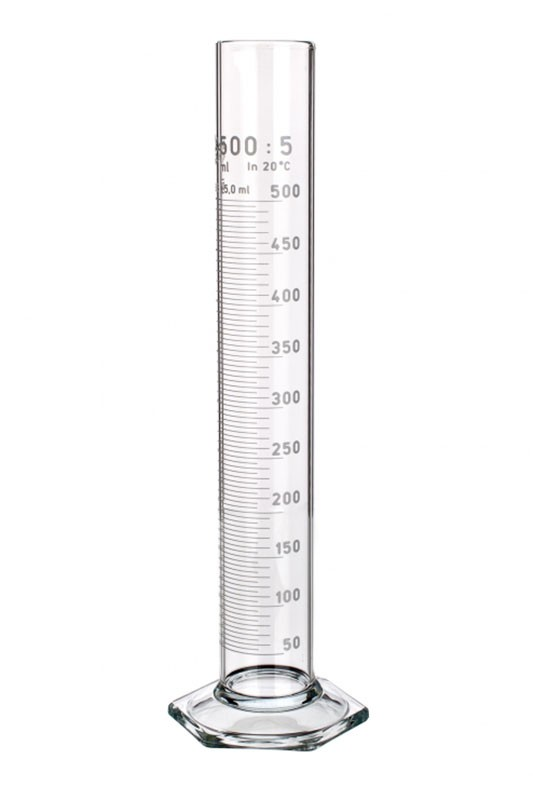
\includegraphics[scale=0.4]{obrazky/odměrný válec.jpg}
    \end{center}
    \caption{Běžný odměrný válec \cite{Odměrný válec}}
\end{figure}
%ZDROJ: https://www.vinarskepotreby.cz/odmerny-valec-1000-ml-sklo.html#gallery


\subsection{Odměrné válce na alkohol}
\label{valec_na_alkohol}

%Ne příliš moc využívanou alternativou jsou válce
%Nepříliš využívaná metoda, zato mnohem efektivnější od klasického válce, kde je nutno alkohol přelévat, zde nám stačí jen láhev s alkoholem položit do středu válce a sledovat stupnici pro měřený alkohol.\\
Nepříliš využívaná metoda, zato mnohem efektivnější od klasického válce jsou odměrné válce na alkohol. Válec obsahuje několik stupnic, obvykle kolem 40, pro různé destiláty. Láhev alkoholu přiložíme k patřičné stupnici a sledujeme rysku, které odpovídá výška hladiny. Tato hodnota je rovna zbytkovému objemu v láhvi. Výhodou této metody je absence přelévání alkoholu.\\

%Lahev alkoholu přiložíme k patřičné stupnici a jaké hodnotě na stupnici od hladiny
%hodnota na stupnici, které je rovna výška hladiny je rovna zbytkovému objemu v láhvi

%Lahev alkoholu prilozime k patricne stupnici a sledujeme rysku, které odpovídá výška hladiny. Tato hodnota je rovna zbytkovému objemu v láhvi. Výhodou této metody je absence přelévání alkoholu.

\textbf{Výhody}
\begin{itemize}
    \item Cenová dostupnost\\
\end{itemize}

\textbf{Nevýhody}
\begin{itemize}
    %\item \textbf{Časově nákladné}
    \item Válec nemusí obsahovat stupnici s požadovaným alkoholem
    \item Změna tvaru láhve - Pokud výrobce alkoholu změní tvar láhve je nutné kupovat nový válec s novou stupnicí
 %(Nový alkohol - pokud v podniku přibide nový destilát k prodeji je nutné koupit válec...)
    \item Nižší přesnost měření\\\\\\\\\\\\\\\\\\
\end{itemize}

\begin{figure}[!h]
    \begin{center}
        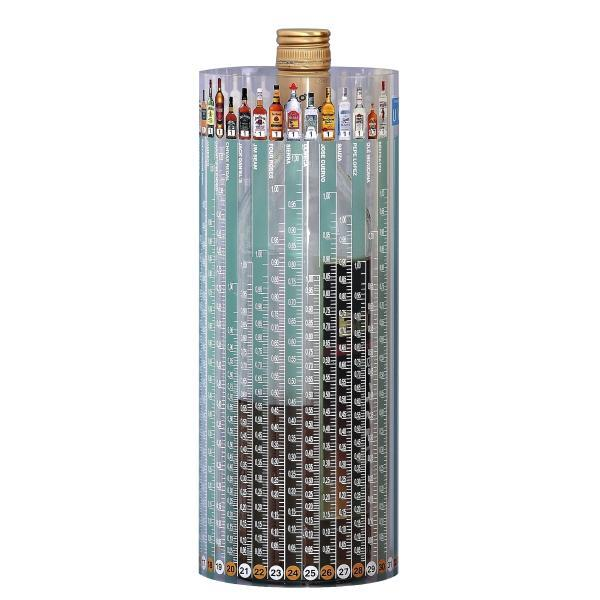
\includegraphics[scale=0.35]{obrazky/odměrný válec na alkohol.jpg}
    \end{center}
    \caption{Odměrný válec na alkohol \cite{Odměrný válec na alkohol}}
\end{figure}

%%Nevyhody:
%zmena tvaru lahve - nutno kupovat nový válec s novou stupnicí
%nepresná hodnota meření

\section{Váhy}
%%foto - mozna
%%Princip přepočtu/výpočtu je podrobneji rozebrán/vice zminen v kapitole [...]

Jedná se o chytré váhy, které na základě databáze s klíčovými daty jsou schopny přepočítat hmotnost měřeného destilátu na jeho objem. 
%Tato problematika je podrobněji rozebrána v kapitole č.3.

Mezi tyto váhy spadá i navrhovaný měřicí systém, který má za úkol inovovat dosavadní měřicí metody.

%Existuje na světě pár společností vyvíjející váhy se stejným účelem. Bohužel jejich využití v praxi je téměř nulové z důvodu neznalosti existence těchto vah a vysoké ceny. Existuji zjednodušené řešení, kdy se využije običejná váha a aplikace pro výpočet objemu, do které se ručně zadá hmotnost destilátu.

%\section{Porovnání}
%
%Válce činí výhodné pouze jedna věc a to pořizovací cena v opačném případě se jedná o velice neefetivní způsob měření. Přes časové a finanční náklady je stále využívána, protože inventura v podnicích není laboratorní...
%
%Měření zbytkového objemu alkoholu v HoReCa podnicích není záležitostí laboratorního výzkumu tedy požadavky na přesnost jsou minimální, klíčovým fakorem je délka/doba inventury.
\chapter{Výpočet objemu - var. 1}
%Hlavní komponentou vyvíjeného systému je váha, kdy z naměřené hmotnosti jsme schopni vypočítat objem. Základní vztah pro výpočet objemu kapaliny je:
Hlavní komponentou vyvíjeného systému je váha, kdy z naměřené hmotnosti jsme schopni vypočítat objem. Použijeme základní vztah pro výpočet objemu, kde hmotnost kapaliny vypočítáme jako rozdíl plné a prázdné láhve:

\begin{equation}
    V = \frac{m}{\rho} \, \left[\mathrm{m^3}\right] \label{objem_kapalina}
 \end{equation}

V ...objem kapaliny

m ...hmotnost kapaliny \([\mathrm{kg}]\)

\(\rho\) ...hustota kapaliny \([\mathrm{kg/m^3}]\)
\\
\\
Výpočet hustoty kapaliny:

%V prvním případě je nutné vypočítat hmotnost kapaliny:

%\begin{equation}
%    m = m_{plná} - m_{prázdná} \, \left[\mathrm{kg}\right]
%    \label{objem_kapalina}
%\end{equation}

%\(m_{min}\) ...hmotnost prázdné láhve \([\mathrm{kg}]\)

%\(m_{max}\) ...hmotnost plné láhve \([\mathrm{kg}]\)
%\\

\begin{equation}
    \rho = \frac{m_{max} - m_{min}}{V_{max}} \, \left[\mathrm{kg/m^3}\right] \label{objem_kapalina}
\end{equation}

\(m_{min}\) ...hmotnost prázdné láhve \([\mathrm{kg}]\)

\(m_{max}\) ...hmotnost plné láhve \([\mathrm{kg}]\)

\(V_{max}\) ...objem plné láhve \([\mathrm{m^3}]\)
\\

%KOMENT

Při výpočtu objemu můžeme zanedbat tepelnou roztažnost ze dvou důvodů:

1)
Při inventarizaci se snažíme zjistit rozdíl v množství destilátu od předchozí inventury. Běžnou praxí je využití odměrného válce, kdy objem určujeme podle rysky. Nový systém však využívá nepřímého měření založeného na hmotnosti. Kapalina při změně objemu nemění svou hmotnost, což vyvolává otázku, proč se nesoustředíme na měření zbytkové hmotnosti místo objemu. V obchodní praxi, a to i v gastronomii, se však všechny lihoviny uvádějí v jednotkách objemu. Proto je nutné naměřenou hmotnost přepočítat na objem, přičemž je klíčové, aby všechny hodnoty byly vztaženy ke stejné teplotě, aby bylo možné výsledky mezi sebou porovnávat. 

Objem se počítá pro referenční teplotu, při které byl stanoven objem plné láhve. Každý kapalný produkt (nápoje, mycí prostředky, oleje atd.) uvádí na své etiketě objem, který je obvykle vypočítán pro pokojovou teplotu 20 °C. Výhodou této metody je, že umožňuje zjistit zbytkové množství kapaliny při jakékoliv teplotě. V případě odměrných válců by bylo nutné měřit všechny destiláty při pokojové teplotě, což je časově náročné(z důvodu než se nám alkohol vytažený z lednice zahřeje na pokojovou teplotu) nebo by bylo potřeba měřit teplotu lihoviny a následně provést korekční výpočet, jaký objem by kapalina měla při pokojové teplotě. Ani jeden z těchto postupů se však běžně nepoužívá kvůli své nepraktičnosti.

2)
V případě odměrných válců jejich nevýhodou je tepelná roztažnost kapalin, kdy válce jsou dimenzované pro konkrétní teplotu, obvykle 20 °C. Většina otevřených destilátů je chlazena v lednicích pro zachování chuti, kvality a aromatu, což způsobuje menší objem naměřený na válci oproti skutečnému. Podmínky skladování si stanovuje každý výrobce lihovin sám. Obvykle čím má lihovina menší procento alkoholu tím se podává chladnější, není to ale pravidlo. Víno je chlazeno na 5 - 15 °C, lihoviny 5 - 18 °C(gin, rum, whisky) a emulzní likéry(vaječný likér, Baileys) > 5 °C.

Například, měří-li se při teplotě 5 °C destilát s vysokým obsahem alkoholu, např. 80\% z důvodu vyšší tepelné roztažnosti ethanolu oproti vodě a při počátečním objemu 1 l, vyjde chyba 13,74 ml za předpokladu, že destilát obsahuje pouze ethanol a vodu bez dalších příměsí. Pro účely inventury však není tato chyba nijak významná. Postup výpočtu je ukázán níže. [\ref{objem_kapalina}]

\begin{equation}
\label{objem_kapalina}
    \Delta V = \Delta V_v + \Delta V_e \left[m^3\right]
\end{equation}


\[\Delta V = 0,64 + 1,13 = 13,74 \left[ml\right]\]


\(\Delta V\) ...celkový rozdílový objem

\(\Delta V_{v}\) ...rozdílový objem vody \([m^3]\)

\(\Delta V_{e}\) ...rozdílový objem ethanolu \([m^3]\)


\begin{equation}
%\label{objem_kapalina}
    \Delta V_v = \frac{p_v}{100} \cdot V_0 \cdot \beta_v \cdot (t_1 - t_0)
\end{equation}

\[\Delta V_v = \frac{20}{100} \cdot 1 \cdot  2,14 \cdot 10^{-4} \cdot (20 - 5) = 0,64 \left[ml\right]\]

\(p_v\) ...objemový podíl vody \([\%]\) 

\(V_0\) ...počáteční objem lihoviny \([m^3]\)

\(\beta_v\) ...součinitel objemové teplotní roztažnosti vody \([\frac{m^3}{m^3 \cdot ^\circ C}]\)

\(t_1\) ...koncová teplota \([^\circ C]\)

\(t_0\) ...počáteční teplota \([^\circ C]\)

\begin{equation}
    \Delta V_e = \frac{p_e}{100} \cdot V_0 \cdot \beta_e \cdot (t_1 - t_0)\left[m^3\right] \label{objem_kapalina}
\end{equation}

\[\Delta V_e = \frac{80}{100} \cdot 1 \cdot  1,09 \cdot 10^{-3} \cdot (20 - 5) = 13,1 \left[ml\right]\]

\(p_e\) ...objemový podíl ethalonu(alkoholu) \([\%]\) 

\(\beta_e\) ...součinitel objemové teplotní roztažnosti ethalonu \([\frac{m^3}{m^3 \cdot ^\circ C}]\)



%\begin{equation}
%    \rho = \frac{m_{plná} - m_{prázdná}}{V_{max}} \, \left[\mathrm{kg/m^3}\right] \label{objem_kapalina}
%\end{equation}


%Výsledný vzorec pro výpočet objemu:

%\begin{equation}
%    V = \frac{m - m_{prázdná}}{\rho} \, \left[\mathrm{m^3}\right] \label{objem_kapalina}
%\end{equation}

%%%%%%%%%%%%%%%%%%%%%%%%%%%%%%%%%%%%%%%%%%%%%%%%%%%%%%%%%%%%%%
%%%%%%%%%%%%%%%%%%%%%%%%%%%%%%%%%%%%%%%%%%%%%%%%%%%%%%%%%%%%%%
\chapter*{Výpočet objemu - var. 2}
\addcontentsline{toc}{chapter}{Výpočet objemu - var. 2}
Hlavní komponentou vyvíjeného systému je váha, kdy z naměřené hmotnosti jsme schopni vypočítat objem. Použijeme základní vztah pro výpočet objemu, kde hmotnost kapaliny vypočítáme jako rozdíl hmotnosti láhve se zbytkovou kapalinou a hmotnosti prázdné láhve:

\begin{equation}
    V = \frac{m - m_{min}}{\rho} \, \left[\mathrm{m^3}\right] \label{objem_kapalina}
\end{equation}

V ...objem kapaliny

m ...hmotnost láhve se zbytkovou kapalinou \([\mathrm{kg}]\)

\(m_{min}\) ...hmotnost prázdné láhve \([\mathrm{kg}]\)

\(\rho\) ...hustota kapaliny \([\mathrm{kg/m^3}]\)
\\
\\
Výpočet hustoty kapaliny:

\begin{equation}
    \rho = \frac{m_{max} - m_{min}}{V_{max}} \, \left[\mathrm{kg/m^3}\right] \label{objem_kapalina}
\end{equation}


\(m_{max}\) ...hmotnost plné láhve \([\mathrm{kg}]\)

\(V_{max}\) ...objem plné láhve \([\mathrm{m^3}]\)
\\
\\
Při výpočtu objemu můžeme zanedbat tepelnou roztažnost ze dvou důvodů:
\\
\begin{enumerate}
    \item
    Při inventarizaci se snažíme zjistit rozdíl v množství destilátu od předchozí inventury. Běžnou praxí je využití odměrného válce, kdy objem určujeme podle rysky. Nový systém však využívá nepřímého měření založeného na hmotnosti. Kapalina při změně objemu nemění svou hmotnost, což vyvolává otázku, proč se nesoustředíme na měření zbytkové hmotnosti místo objemu. V obchodní praxi, a to i v gastronomii, se však všechny lihoviny uvádějí v jednotkách objemu. Proto je nutné naměřenou hmotnost přepočítat na objem, přičemž je klíčové, aby všechny hodnoty byly vztaženy ke stejné teplotě, aby bylo možné výsledky mezi sebou porovnávat.
    
    Objem se počítá pro referenční teplotu, při které byl stanoven objem plné láhve. Každý kapalný produkt (nápoje, mycí prostředky, oleje atd.) uvádí na své etiketě objem, který je obvykle vypočítán pro pokojovou teplotu 20 °C. Výhodou této metody je, že umožňuje zjistit zbytkové množství kapaliny při jakékoliv teplotě. V případě odměrných válců by bylo nutné měřit všechny destiláty při pokojové teplotě, což je časově náročné(z důvodu než se nám alkohol vytažený z lednice zahřeje na pokojovou teplotu) nebo by bylo potřeba měřit teplotu lihoviny a následně provést korekční výpočet, jaký objem by kapalina měla při pokojové teplotě. Ani jeden z těchto postupů se však běžně nepoužívá kvůli své nepraktičnosti.
    
    \item 
    %Z výše uvedeného bodu vyplývá, že vypočítaný objem bude odpovídat referenční teplotě 20 °C. Stejně jako v příkladu č. [\ref{objem_kapalina}] se objeví zanedbatelná chyba, pokud bude měřicí systém stejně nebo přesnější než odměrný válec.
    I pro případ, kdybychom nepočítali objem pro referenční teplotu, tak odchylka vyjde stejně jako v příkladu č. [\ref{objem_kapalina}], kde se objeví zanedbatelná chyba, pokud bude měřicí systém stejně nebo přesnější než odměrný válec.
\end{enumerate}



%%%%%%%%%%%%%%%%%%%%%%%%%%%%%%%%%%%%%%%%%%%%%%%%%%%%%%%%%%%%%%
%%%%%%%%%%%%%%%%%%%%%%%%%%%%%%%%%%%%%%%%%%%%%%%%%%%%%%%%%%%%%%

\chapter*{Přepočet hmotnosti na objem}
\addcontentsline{toc}{chapter}{Přepočet hmotnosti na objem}
\label{Přepočet hmotnosti na objem}
%Přepočet hmotnostního množství na objemové / Výpočet objemu
%\section{Princip}

%Hlavní komponentou vyvíjeného systému je váha, která slouží, stejně jako víše zmíněne váhy, k přepočtu hmotnostního množství na objemové.
%Ze známe hmnotnosti 

%Hlavní komponentou vyvíjeného systému je váha, která slouží k přepočtu hmotnostního množství na objemové. Základní vztah pro výpočet objemu je: 

%Hlavní komponentou vyvíjeného systému je váha, kdy z naměřené hmotnosti jsme schopni vypočítat objem. Základní vztah pro výpočet objemu kapaliny je:

%\begin{equation}
%    V = \frac{m}{\rho} \, \left[\mathrm{m^3}\right] \label{objem_kapalina}
%\end{equation}

%V ...objem kapaliny

%m ...hmotnost kapaliny \([\mathrm{kg}]\)

%\(\rho\) ...hustota kapaliny \([\mathrm{kg/m^3}]\)
%\\

%V praxi by byla tato metoda poměrně přesná pro výpočet objemu pouze čirých destilátů, které mají složení “jen” vody a ethanolu, pro které známe hustotu a poměr mezi nimi, díky známé hodnotě obsahu alkoholu. Barevné destiláty nebo destiláty s vyšší viskozitou obvykle obsahují další příměsi, pro které neznáme jejich hustotu a poměr mezi nimi a výpočet pouze z vody a ethanolu by vedl na velkou chybovost.
%Tato metoda by byla v praxi poměrně přesná pro výpočet objemu pouze čirých destilátů, které se skládají "jen" z vody a ethanolu. Pro tyto destiláty známe hustotu a poměr obou složek díky známému obsahu alkoholu. Barevné nebo viskózní destiláty však obvykle obsahují další příměsi, jejichž hustotu a poměr neznáme. Výpočet pouze z vody a ethanolu by proto vedl k velké nepřesnosti.

\section{Linearizace}
\label{odkazos}
%https://cs.wikipedia.org/wiki/ISO_1
%https://cs.wikipedia.org/wiki/Standardn%C3%AD_teplota_a_tlak

Pro výpočet objemu kapaliny, v našem případě destilátů, můžeme za určitých podmínek použít linearizaci dvou bodů. Výpočet provedeme ze známého objemu plné láhve a hmotnosti prázdné a plné láhve. Teplota a tlak nemají vliv na hmotnost, tedy na množství alkoholu, a proto je můžeme zanedbat. Výsledný objem bude platit pro referenční teplotu a tlak, při kterých byl stanoven objem plné láhve.

%Výpočet objemu kapaliny v našem případě destilátů se dá za určitých podmínek spočítat pomocí linearizace dvou bodů %- hmotnosti prázné a plné lahve a k tomu patřičný objem.

%Výpočet budem provádět ze známého objemu plné láhve a naměřené hmotnosti prázdné a plné láhve. Teplota a tlak nemá vliv na naměřenou hmotnost tedy množství alkoholu a můžeme je zanedbat. Výsledný objem bude pro referenční teplotu a tlak při které byl stanoven objem plné láhve. %Pro naše účely tedy není nutné znát objem v daném okamžiku, ale za  

%Tuhle teplotu a tlak stanovuje česká norma ČSN EN ISO 1 (01 4110).

%Výpočet je tedy závislý na naměřené hmotnosti na kterou nemá vliv teplota ani tlak. 

%Tím, že je výpočet závislý na hmotnosti, tak můžeme zanedbat teplotu a tlak. Rozdílem hmotností kapaliny a láhve jsme schopni získat  

%Teplotu a tlak můžeme zanedbat. Tím, že měříme hmotnost 

%Při fyzické inventuře nás zajímá skutečné množství  


%V našem případě tlak v uzavřené láhvi je tak malý, že neovlivňuje výsledný objem kapaliny. Teplota 

%inventurní účely se dá  
%
%však můžem použít jinou metodu, která není závislá na hustotě, tedy teplotě a tlaku s tím spojená. 
%
%%Hustota je závislá na teplotě, proto budem počítat s její referenční hodnotou teploty. Budem předpokládat, jaký 
%%Našim cílem je po
%
%Hustota je závislá na teplotě a tlaku. V případě kapalin můžeme tlak zanedbat z důvodu "nulového" vlivu na výsledný objem.
%
%V praxi
%
%Hustota je závislá na teplotě a tlaku, proto si stanovíme pevnou hodnotu teploty, kterou budem považovat za konstantu. Budem tedy počítat objem kapaliny pro referenční teplotu a tlak. Náš objem tedy bude závisly pouze na hmotnosti a můžeme ho linearizovat.
%
%Našim cílem je změřit objem alkoholu bez nutnosti jej přelévat, proto budem měřit i hmotnost lahve ve kterém se alkohol nachází. Ze známe hmotnosti prázdné "m1" a plné láhve "m2 "a tomu příslušnému objemu 'V2', jsme schopni vytvořit předpis přímky ze dvou bodů. %V první řadě je nutné zjistit směrnici (pro nulový offset):

Výpočet objemu pomocí předpisu přímky ve směrnicovém tvaru:
\begin{equation}
    V = k \cdot m - q\, \left[\mathrm{m^3}\right] \label{objem_linearizace}
\end{equation}

Výpočet směrnice:
%\ref{objem_linearizace}
\begin{equation}
    k = \frac{V_{max}-V_{min}}{m_{max}-m_{min}}\, \left[\mathrm{m^3/kg}\right]\label{směrnice}
\end{equation}

\(V_{min}\) ...objem prázdné láhve \([\mathrm{m^3}]\)

\(V_{max}\) ...objem plné láhve \([\mathrm{m^3}]\)

\(m_{min}\) ...hmotnost prázdné láhve \([\mathrm{kg}]\)

\(m_{max}\) ...hmotnost plné láhve \([\mathrm{kg}]\)
\\

Objem prázdné lahve bude vždy nulový, proto můžeme předpis směrnice zjednodušit:
\begin{equation}
    k = \frac{V_{max}}{m_{max}-m_{min}}\, \left[\mathrm{m^3/kg}\right] \label{směrnice_ez}
\end{equation}

%Pokud to nepujde napsat vizuálně zlomkovým tvarem, tak dat nezapomenout závorky

Výpočet offsetu:
\begin{equation}
    q = V_{min} - k \cdot m_{min}\, \left[\mathrm{m^3}\right] \label{offset}
\end{equation}

Opětovně jde zjednodušit na tvar:

\begin{equation}
    q = k \cdot m_{min}\, \left[\mathrm{m^3}\right] \label{offset_ez}
\end{equation}

%Pro naší aplikaci bude V1 vždy rovna nule, protože minimální objem je nulový

%%FOTO grafu ve kterem bude Vmin = 0

%\section{Linearizace}
\chapter{Sériová komunikace}
\label{Sériová komunikace}

%Sériová komunikace je posílání dat v řadě nebo-li bit po bitu
Seriová komunikace je způsob přenosu dat mezi dvěma nebo více zařízeními, při kterém se data posílají po jednotlivých bitech po jediném vodiči nebo bezdrátovém kanálu. Seriová komunikace je vhodná pro dlouhé vzdálenosti a nižší rychlosti, protože vyžaduje méně vodičů než paralelní komunikace, která se běžně využívá na deskách plošných spojů. Seriová komunikace se dělí na synchronní a asynchronní, podle toho, zda je potřeba precizně synchronizovat časování při vysílání mezi vysílačem a přijímačem. Pro naše účely se budem zabývat pouze asychronní komunikací. Seriová komunikace se používá pro různé účely, jako je komunikace s modemem, tiskárnou, senzory, paměťovými kartami, síťovými adaptéry a dalšími periferiemi. Běžné a obecně známé standardy a protokoly pro seriovou komunikaci jsou RS-232, UART, SPI, USB.
%...precizně synchronizovat časování při vysílání mezi vysílačem a přijímačem (tohle poradil Pety)
\cite{ser kom}
%[zdroj]
%zdroj kniha o seriove komunikaci
\begin{figure}[!h]
    \begin{center}
        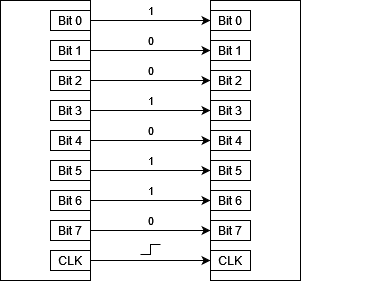
\includegraphics[scale=0.62]{obrazky/paralelni_komunikace.png}
        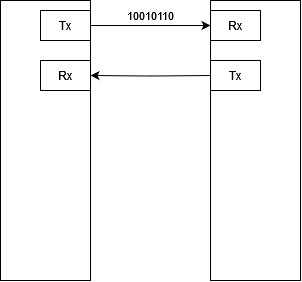
\includegraphics[scale=0.62]{obrazky/Seriova komunikace.png}
    \end{center}
    \caption[Porovnání seriové a paralelní komunikace]{Porovnání paralelní(vlevo) a sériové(vpravo) komunikace. Sériová komunikace v topologii pro UART protokol}
\end{figure}
%zdroj: https://www.rohde-schwarz.com/cz/products/test-and-measurement/essentials-test-equipment/digital-oscilloscopes/understanding-serial-protocols_254522.html#gallery-5

%\section{Komunikační protokoly}
%Komunikační protokol je sada pravidel a dohod, které umožňují zařízením komunikovat mezi sebou. Protokol definuje formát, obsah, časování a řízení toku dat mezi odesílatelem a příjemcem. \cite{ser kom}

\section{UART protokol}
Komunikační protokol je sada pravidel a dohod, které umožňují zařízením komunikovat mezi sebou. Protokol definuje formát, obsah, časování a řízení toku dat mezi odesílatelem a příjemcem.

UART (Universal asynchronous receiver - transmitter) protokol je jeden z nejstarších a nejjednodušších komunikačních protokolů, který používá sériovou linku pro přenos dat mezi dvěma zařízeními. UART protokol nemá společný hodinový signál, ale zařízení se mezi sebou jinými prostředky dohodnou na rychlosti přenosu (baud rate) a formátu dat (počet bitů, parita, stop bit). UART protokol používá čtyři signály: TX (vysílač), RX (přijímač), GND (zem) a volitelně RTS/CTS (řízení toku). \cite{ser kom} %UART protokol je často používán pro komunikaci s periferními zařízeními, jako jsou modemy, senzory, displeje nebo klávesnice. \cite{ser kom}

\subsection{UART datový paket}
\label{UARTt}
Datový paket popisuje posloupnost nebo-li datový tok bitů. Z obrázku č. \ref{UART packet} je vidět, že paket je ohraničený START(logická úrověň 1) a STOP(logická úrověň 0) bitem, které udávají začátek a konec zprávy. Díky tomu jsme schopni separovat více jdoucích paketů v řadě. Za START bitem následuje datový rámec, který býva z pravidla 8 bitový (1 Bajt) a nese informaci uživatele, ostatní bity slouží k "řízení" paketu. Dále je zde paritní bit, který aplikuje na datový rámec logickou operaci XOR. Existují dva druhy parity: sudá - XOR operace je rovna 1 pokud počet jedniček v datovém rámci je sudý.  Pro lichou paritu platí to stejné v případě, že počet jedniček v rámci je lichý. Paritní bity nejsou vždy využity. Záleží na konkrétní aplikaci. Slouží ke kontrole, jestli datový rámec není poškozen. \cite{ser kom} %[zdroj:] %https://cs.wikipedia.org/wiki/Paritn%C3%AD_bit
%*XOR je 

\begin{figure}[!h]
    \begin{center}
        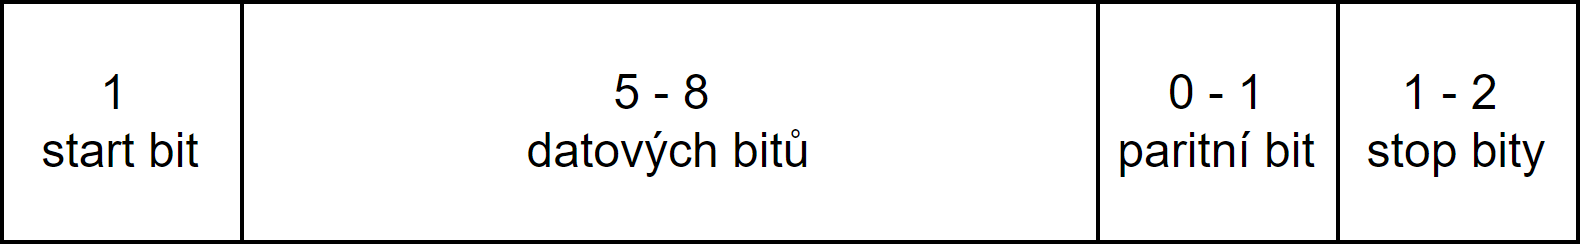
\includegraphics[scale=0.5]{obrazky/datovy ramec UART - final.png}
    \end{center}
    \caption{Datový tok protokolu UART}
    \label{UART packet}
\end{figure}
%ZDROJ: https://yarkov.tech/en/blog/2022-11-04/using-the-web-serial-api-to-communicate-with-the-microcontroller/

\section{Standard RS-232}
Komunikační standard je soubor pravidel a specifikací, které definují, jak mají zařízení komunikovat mezi sebou. Komunikační standard zahrnuje fyzické, elektrické, funkční a mechanické charakteristiky komunikačního rozhraní. Například RS-232 je komunikační standard pro sériovou komunikaci mezi počítačem a modemem.
RS-232 definuje:
\begin{itemize}
    \item \textbf{Elektrické charakteristiky:} RS-232 používá napěťové úrovně od -15 V do +15 V pro reprezentaci logických stavů 0 a 1. RS-232 také specifikuje maximální rychlost přenosu, impedanci, toleranci zkratu a další parametry signálu.
    \item \textbf{Funkční charakteristiky:} RS-232 popisuje funkce a smysl definovaných signálů, které se používají pro řízení toku dat mezi zařízeními. Některé z těchto signálů jsou například: TXD (odesílaná data), RXD (přijímaná data), RTS (požadavek na odeslání), CTS (povolení k odeslání) a DTR (připraven k zařízení).
    \item \textbf{Mechanické charakteristiky:} RS-232 definuje také fyzický tvar a rozmístění pinů konektorů, které se používají pro propojení zařízení. Nejběžnějšími typy konektorů jsou DB9 a DB25, které mají devět a pětadvacet pinů, viz obrázek č.\ref{rs232_obr} \cite{ser kom}
\end{itemize}
%Zdroj dokument o seri. komunikaci

\begin{figure}[!h]
    \begin{center}
        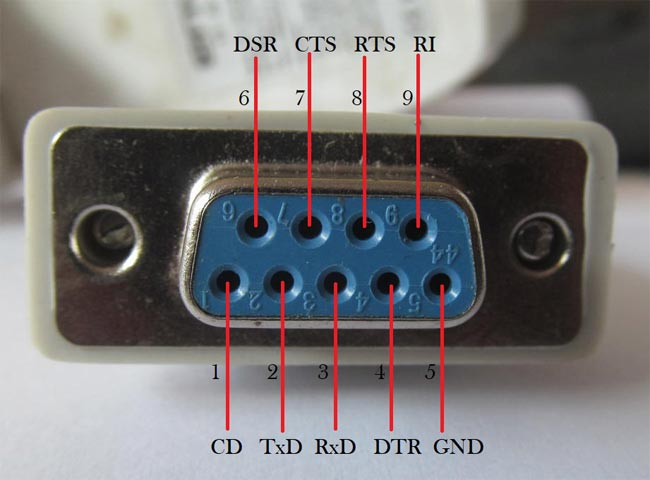
\includegraphics[scale=0.4]{obrazky/RS232.jpeg}
    \end{center}
    \label{rs232_obr}
    \caption{Konektor DB9 s popisem pinů. \cite{RS232}}
\end{figure}
%zdroj RS-232: https://www.pbxdom.com/blog/engineering/what-is-serial-rs232-port-interface/

%\section{USB}
%Universal Serial Bus zkráceně USB je průmyslový standard, který stanovuje specifikace pro kabely a konektory na zařízeních, stéjně jako výše zmíněné RS-232.
%
%USB diponuje konektory Vcc (napájení 5V), datovými piny D+ (vysílač), D- (přijímač) a GND(zem). Obsahuje další konektory jako superrychlostní datové piny, ale těmi se zabívat nebudeme.
%
%Existuje několik verzí USB, které se od sebe líší jak fyzickými rozměry(tvarem konektoru) tak i přenosovou rychlostí. My se budem zabívat verzí USB 2.0 a 3.x s konektorem typu A
%
%USB přišlo jako "náhrada" za starší standard RS-232. USB je rozměrově menší a několika násobně rychlejší.[zdroj]
%%zdroj ai, citoval wikinu
%
%%asi vymazat tuhle sračku
%\begin{figure}[!h]
%    \begin{center}
%        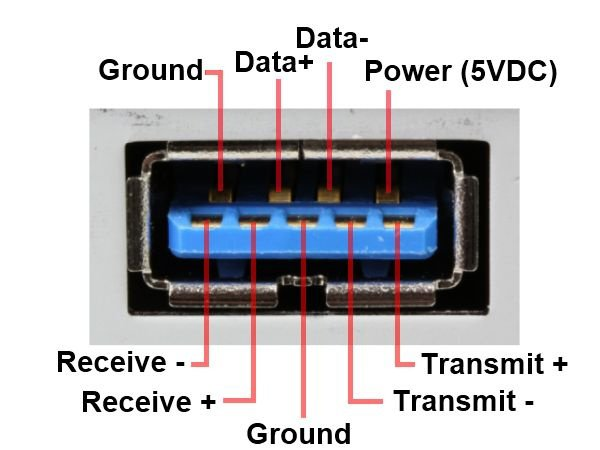
\includegraphics[scale=0.4]{obrazky/USB.jpg}
%    \end{center}
%    \caption{USB 3.1/3.2 A s popisem pinů}
%\end{figure}
%%zdroj USB: https://www.quora.com/If-USB-3-0-type-A-support-max-output-at-5v-0-9a-why-are-there-so-many-type-A-to-type-C-cables-that-supposedly-support-5v-3a
%%Doporuceno zmenit zdroj
\chapter{Nově navržený systém}
\label{Nově navržený systém}
%V této kapitole se budem zabívat nově navrženým systémem, jejíma komponentama a... 
Nově navržený systém se skládá z databáze a 5 hlavních komponent navzájem propojených: modul s výpočetní jednotkou, váha, čtečka čárového kódu a dotykový displej. Dále je možnost připojit systém k počítači pro správu databáze a tisk dat. 

\section{Postup měření}%/Princip/funkcionalita
Pro evidenci zůstatkového objemu jedné láhve je nutné naskenovat její čárový kód pomocí čtečky čárových kódů a zvážit ji. Mikrokontroler na základě získaného EAN vybere z databáze patřičná data, viz kapitola č. \ref{databaze} a přepočítá hmotnost na objem. V případě, že by čárový kód nebyl čitelný, je možné ho zadat ručně do systému prostřednictvím klávesnice. Veškeré důležité informace včetně zbytkového objemu se zobrazí na displeji. %Pro výpis všech naměřených dat je možné systém připojit k počítači a nechat si je vytisknout do formátu .xlsx pomocí navržené desktopové aplikace. Tato aplikace slouží i ke správě databáze.
%Do budoucna k měřicimu systému bude vyvíjena desktopová aplikace běžící na stolním počítačí/notebooku. Mikrokontroler bude k počítači připojen prostřednictvím USB portu
%Do budoucna pro výpis všech naměřených dat bude možné systém připojit k počítači a nechat si je vytisknout do formátu  .xlsx pomocí navržené desktopové aplikace. Tato aplikace slouží i ke správě databáze.

Do budoucna bude vyvíjena desktopová aplikace pro editaci databáze[č.5.3] a zpracování naměřených dat, jako je například tisk do formátu .xlsl. Měřící systém bude propojený s počítačem skrz USB kabel nebo Wi-Fi.

\section{Blokové schéma}
%FOTO
%Výpočetní jednotka Raspberry pi pracuje s databázi dat jednotlivých destilátů. V první řadě je nutné tuhle databází vytvořit a implementovat prostřednictvím desktopové aplikace. 
\begin{figure}[!h]
    \begin{center}
        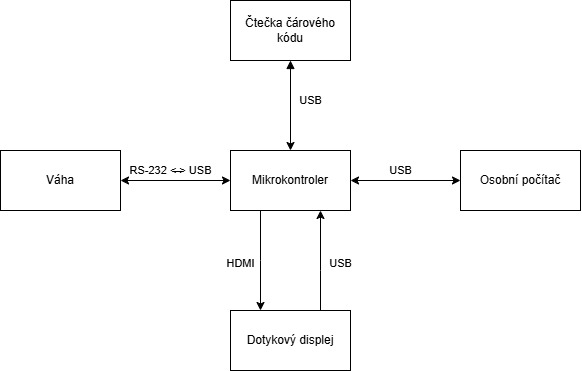
\includegraphics[scale=0.7]{obrazky/Blokové schéma.jpg}
    \end{center}
    \label{blokove_schema}
    \caption{Blokové schéma nově navrženého systému}
\end{figure}

\section{Databáze}
\label{databaze}
%Celý systém je závislý na datech, které nesou informace o názvu destilátu
Aby bylo možné přepočítat hmotnost na objem je nutné znát předem hmotnost prázdné a plné láhve a její maximální objem. Postup výpočtu je zmíněn v kapitole č. \ref{odkazos}. Tyto data jsou uloženy v relační\footnote{Data uložený v tabulkách, kde sloupce reprezentují atributy a řádky jednotlivé záznamy, řádky jsou propojeny pomocí tzv. klíčů. Tabulky \ref{databaze_destilatu} a \ref{tab:my_label} mají prohozené řádky a sloupce z důvodu lepšího umístění na stránku.} databázi včetně informací jako jsou: název destilátu, EAN kód, maximální objem, nebo adresa k obrázku daného produktu.
%K datům se přistupuje pomocí EAN kódu nebo názvem destilátu zadaný klávesnicí.

%Některé destiláty, mají na svém hrdle nalévač místo vršku, který mění hmotnost láhve. Aby naš systém byl časově efektivní, tak implementujeme druhou databázi 

%Některé destiláty mají na svém hrdle nalévátko (obrázek č. \ref{nalevačos}) místo víčka, který mění hmotnost láhve. V takovém případě bychom museli nalévač nahradit víčkem, aby hmotnost láhve odpovídala předpisu funkce, což je časově neefektivní. Místo toho byla navržena druhá databáze, obsahující hmotnosti různých nalévačů. Vzorec pro výpočet objemu ve výchozím nastavení počítá s víčkem na láhvi, proto uživatel musí při měření zakliknout pomocí klávesnice, že chce měřit objem s nalévačem. Při výpočtu dojde k nahrazení hmotnosti víčka hmotností nalévače a následně dojde k výpočtu výsledného objemu.

Některé destiláty mají na svém hrdle nalévač nebo také nalévátko (obrázek č. \ref{nalevačos}) místo víčka, který mění hmotnost láhve. V takovém případě bychom museli nalévač nahradit víčkem, aby hmotnost láhve odpovídala předpisu rovnice č.xyz (skutečná hmotnost prázdné láhve musí odpovídat s hodnotou hmotnosti prázdné láhve v databázi), což je časově neefektivní. Místo toho byla navržena druhá databáze, obsahující hmotnosti různých nalévačů. Vzorec pro výpočet objemu ve výchozím nastavení počítá s víčkem na láhvi, proto uživatel musí při měření zakliknout v aplikaci, že chce měřit objem s nalévačem. Při výpočtu dojde k nahrazení hmotnosti víčka hmotností nalévače a následně dojde k výpočtu výsledného objemu.


%Vyhledání destilátu a jeho dat je porstřednictvím EAN kódu nebo jeho názvu.

Obě databáze jsou uložené v mikrokontroléru.

%FOTO
\begin{table}[!h]
\centering
\begin{tabular}{|l|l|l|l|}
\hline
 & Destilát č. 1   & Destilát č. 2   &  . . . \\ \hline
\textbf{Název destilátu} [-] [\textit{TEXT}] &   &    &  \\ \hline
\textbf{EAN kód} [-] [\textit{INTEGER}]&  &    &        \\ \hline
\textbf{Hmotnost prázdné láhve} [g] [\textit{numeric}] &    &  &        \\ \hline
\textbf{Hmotnost plné láhve} [g] [\textit{numeric}] &    &    &  \\ \hline
\textbf{Hmotnost víčka} [g] [\textit{numeric}] &    &    &  \\ \hline
\textbf{Maximální objem láhve} [l] [\textit{numeric}] &    &    &  \\ \hline
\textbf{Množství alkoholu} [\%] [\textit{numeric}] &    &    &  \\ \hline
\textbf{Adresa obrázku} [-] [\textit{TEXT}] &    &    &  \\ \hline
%Obrázek: obsahuje adresu/název obrázku, který je uložen ve složce
\end{tabular}
\label{databaze_destilatu}
\caption{Databáze destilátů}
\end{table}


\begin{table} [!h]
    \centering
    \begin{tabular}{|l|l|l|l|}
    \hline
         & Nalévač č. 1 & Nalévač č. 2 &  . . .\\ \hline
         \textbf{Název nalévače} [-] [\textit{TEXT}] & & &\\ \hline
         \textbf{Výrobce} [-] [\textit{TEXT}] & & &\\ \hline
         \textbf{Hmotnost} [g] [\textit{numeric}] & & &\\ \hline
         \textbf{Adresa obrázku} [-] [\textit{TEXT}] & & &\\ \hline
    \end{tabular}
    \caption{Databáze nalévačů}
    \label{tab:my_label}
\end{table}

\begin{figure}[!h]
    \begin{center}
        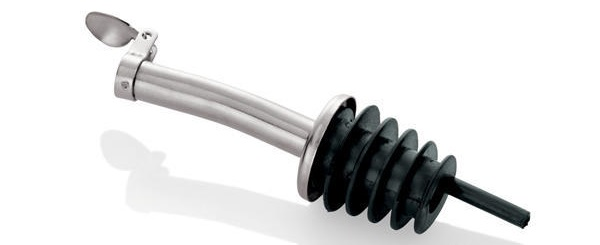
\includegraphics[scale=0.6]{obrazky/nalevac.jpg}
    \end{center}
    \label{nalevačos}
    \caption{Nalévač na alkohol \cite{nalevatko}}
\end{figure}
% \definecolor{Silver}{rgb}{0.752,0.752,0.752}
% \begin{table}[!h]
%     \centering
%     \begin{tabular}
%         {
%         cell{1}{4} = {c},
%         hlines = {Silver},
%         vlines = {Silver},
%         }
%         Název & hmotnost\\
%         Nalévač č.1 & x\\
%     \end{tabular}
%     \caption{Caption}
%     \label{tab:my_label}
% \end{table}
%\usepackage{color}
%\usepackage{tabularray}
%\definecolor{Silver}{rgb}{0.752,0.752,0.752}
%\begin{tabular}[
%  label = none,
%  entry = none,
%]{
%  cell{1}{4} = {c},
%  hlines = {Silver},
%  vlines = {Silver},
%}
%Název destilátu & destilát č.1 & destilát č.2 & . . . \\
%EAN kód & & & \\
%hmotnost prázdné láhve & & & \\
%hmotnost plné láhve    &              & & \\
%hmotnost víčka         &              &              &       \\
%obrázek                &              &              &       \\
%max. objem             &              &              &       
%\end{tabular}
%Tabulka destilátů
%Nazev | EAN | k | q | m_víčko | max_objem | obrazek | poznamka
%Tabulka druhů nalévačů
%Nazev | m_nalevač | obrazek

\section{Váha}

Nejdůležitější komponentou systému je váha pro výpočet zbytkového objemu z naměřené hmotnosti láhve, viz kapitola č.\ref{Přepočet hmotnosti na objem}.  Proto v této podkapitole rozeberu požadavky, výběr váhy a její alternativy.
%
%Váhy jsou zařízení, která slouží k měření hmotnosti objektů. Existuje mnoho typů vah, ale základní princip je stejný. Váhy se skládají ze dvou hlavních částí: měřicího mechanismu a zobrazovacího mechanismu.
%
%Měřicí mechanismus se skládá z vážícího tělesa a pružiny. Když položíte objekt na váhu, pružina se stlačí a vážící těleso se posune dolů. Tento pohyb se přenáší na měřicí stupnici, která ukazuje hmotnost objektu.
%
%Zobrazovací mechanismus se skládá z displeje a elektronického obvodu. Elektronický obvod přijímá signál od měřicího mechanismu a převádí ho na čitelný formát pro displej. Displej pak zobrazuje hmotnost objektu.[zdroj]
%
%\subsection{Elektronická část váhy}
%
%Elektronická část váhy se skládá z senzoru a elektronického obvodu. Senzor měří deformaci, kterou způsobuje vážený objekt, a převádí ji na elektrický signál. Tento signál je poté zpracován elektronickým obvodem, který obsahuje A/D převodník a mikroprocesor.
%
%Senzory používané v elektronických vahách jsou obvykle tenzometry nebo load cells. Tenzometry jsou malé senzory, které měří změnu odporu, když jsou deformovány. Load cells jsou senzory, které měří změnu napětí, když jsou deformovány. Oba typy senzorů jsou velmi přesné a umožňují měření hmotnosti s vysokou přesností.
%
%A/D převodník převádí analogový signál z senzoru na digitální signál, který může být zpracován mikroprocesorem. Mikroprocesor pak zpracovává signál a zobrazuje výslednou hmotnost na displeji. [zdroj]
%
\subsection{Požadavky na váhu}

%Dle výpočtů[], aby systém splnil toleranci +-5ml je nutné volit váhu s přesností menší jak 0,075g, tomu z dostupných vah na trhu odpovídá váha s přeností 0,01g, kde výsledná přesnost měřícího systému pro metodu x je pod limitem přesnosti válce třídy A a nebo přesnost 0,1g, kde jsem na hraně.
%Další možností jak 

%bude pro metodu č. x XY+-ml a pro metodu a nebo o něco méně přesná 0,1 g, kde výsledná přesnost vychází +-5,2 ml

%Z komerčních důvodů byla vybrána váha s přesností 0,5g, kde přesnost celého systému 

%Tabulka: metoda(A,B,C), přesnost váhy(C=2váhy), přesnost systému, cena

Hlavním požadavkem je oboustranný otevřený komunikační port pro čtení dat a odesílání požadavku na jejich zaslání prostřednictvím sériové linky do řídící jednotky, je tedy nutné znát přesný popis přenosu dat. Tyto požadavky zpravidla splňují laboratorní a průmyslové váhy, kde se očekává, že data budou zpracovávána pomocí aplikačního softwaru.

Váživost (maximální hmotnost, která lze na váze navážit) se požaduje minimálně 2 kg. Hmotnost prázdné láhve u většiny destilátů se pohybuje od 500 do 800 g a samotný obsah láhve je od 500 do 1000 ml, tudíž až necelý 1 kg. V případě robustnějších lahví okolo 1 kg by váživost do 2 kg nemusela stačit, proto je vhodnější volit 3 kg. Větší váživost jak 3 kg, by neměla pro běžné podniky HoReCa význam, navíc s vyšší váživostí úměrně klesá její přesnost a roste cena váhy.

Přesnost, jinak řečeno rozlišení nebo odčitatelnost, se udává v dílcích(d). Dílek je nejmenší hodnota hmotnosti, kterou lze z displeje váhy odečíst.\cite{vazivost} Měření zbytkového objemu destilátu při inventurách není záležitostí "laboratorního měření" a zákon nestanovuje s jakou přesností je nutné měřit objem v láhvích pro inventurní účely. Obecně na 
přesnost není kladen velký důraz. Tím, že žádná norma nestanovuje, jakou přesnost by měl mít nově navržený měřicí systém, by bylo optimální, aby měřilo s přesností stejnou nebo vyšší než odměrné válce. Odměrné válce na alkohol
(kapitola č. \ref{valec_na_alkohol}) mají přesnost ±5 ml. Obyčejné odměrné válce (kapitola č. \ref{obecny_valec}) třídy B mají přesnost ±10 ml a třídy A ±5 ml.

Požadovaná přesnost váhy závisí na hustotě měřené kapaliny.  Čím hustší kapalinu máme, tím menší přesnost vyžadujeme, a naopak - méně hustá kapalina bude vážit méně na jednotku objemu, v našem případě 10 ml. Tudíž nás zajímá, která složka destilátu má nejmenší hustotu. Ve své podstatě bude měřen pouze ethanol a voda, co se týče příměsí pro dochucení, tak ty jsou větší hustoty, proto přesnost váhy vztáhneme k ethanolu, i když nikdy nebudeme měřit 100\% ethanol, ale jeho směs s vodou a dalšími příměsi. Požadovaná přesnost váhy tedy je ±3,95 g (10 ml ethanolu), postup výpočtu níže[\ref{presnost vahy}]:\\

Výpočet přesností váhy:
%\begin{equation}
%    Presnost\, váhy = \frac{V_{max}-V_{min}}{m_{max}-m_{min}}\, \left[\mathrm{m^3/kg}\right]\label{presnost vahy}
%\end{equation}

%\begin{equation}
%    Přesnost\ váhy = Přesnost\ válce \cdot Hustota\ kapaliny \label{presnost vahy}
%\end{equation}

\begin{equation}
    %U(m) = U(V) \cdot \rho 
    \Delta m = \Delta V \cdot \rho \label{presnost vahy}
\end{equation}

\(\Delta m\) ...Přesnost váhy \([\mathrm{g}]\) %Nejistota hmotnosti (přesnost váhy)

\(\Delta V\) ...Přesnost válce \([\mathrm{ml}]\) %...Nejistota objemu (přesnost válce)

\(\rho\) ...Hustota nejlehčí složky destilátu (ethanol) \([\mathrm{g/ml}]\)

\begin{equation}
    \Delta m = \pm5 \cdot 0,79 = \pm3,95 \, \left[\mathrm{g}\right] \label{presnost vahy}
\end{equation}



Váha je určena pro fyzickou inventuru HoReCa podniků, která spadá pod interní činnost podniku a není podmínkou, aby byla certifikována viz. kapitola č.\ref{meridlo}
%Váha je určena pro interní chod podniku a není podmínkou, aby byla certifikována.

Po splnění výše zmíněných požadavků je rozhodujícím faktorem cena.
\\ \\
%zdroj: https://www.hepnar.cz/poradna/view/co-je-to-max-vazivost-a-dilek/
%Posledním parametrem je cena, kdy
%Váha by měla být kompaktní, aby ji bylo možné
%Při inventurách je hlavním problémem časová náročnost a 
%Přesnost v našem případě není až tak důležitou vlastností
\textbf{Souhrn požadavků prioritně seřazených:} %sestupně / 
\begin{itemize}
    \item Oboustranný otevřený komunikační port
    \item Váživost nad 2 kg
    \item Přesnost ±3,95 g a více
    \item Nízká cena
\end{itemize}

\subsection{Vybraná váha}
%Při výběru váhy jsem se řídil výše zmíněnými požadavky, kdy. 

Váha byla vybrána na základě výše zmíněných požadavků.
Základní parametry váhy jsou vyobrazené v tab. č \ref{vahaa}.
%Kompletní dokumentace je v příloze č. x
Kompletní specifikace je uvedena v dokumentaci: \cite{vaha_datasheed}



\begin{table}[!h]
    \centering
    \begin{tabular}{|c|c|}
        \hline
        Výrobce                                                         & G\&G   \\ \hline
        Model                                                           & E3000  \\ \hline
        %\begin{tabular}[c]{@{}c@{}}Komunikační\\ protokol\end{tabular}  & UART   \\ \hline
        \begin{tabular}[c]{@{}c@{}}Komunikační \\ rozhraní\end{tabular} & RS-232 \\ \hline
        \begin{tabular}[c]{@{}c@{}}Datový \\ konektor\end{tabular} & \begin{tabular}[c]{@{}c@{}}DE-9\\ (Samice)\end{tabular} \\ \hline
        Váživost                                                        & 3 kg    \\ \hline
        Přesnost                                                        & 0.5 g     \\ \hline
        \begin{tabular}[c]{@{}c@{}}Doba \\ stabilizace\end{tabular} & < 2 s \\ \hline
        Cena                                                            & 1987 Kč     \\ \hline
    \end{tabular}
    \label{vahaa}
    \caption{Základní parametry vybrané váhy}
\end{table}

\begin{figure}[!h]
    \begin{center}
        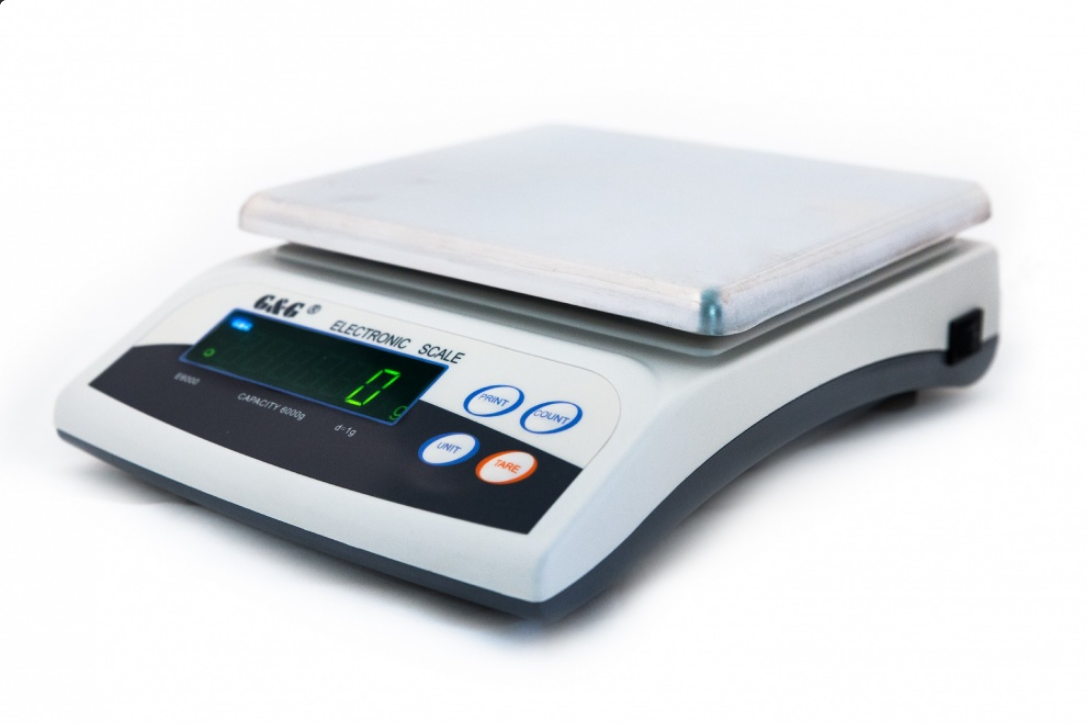
\includegraphics[scale=0.25]{obrazky/E3000.png}
    \end{center}
    \caption{Vybraná váha G\&G E3000 \cite{vaha}}
\end{figure}



% Jeden z hlavních požadavků bylo, aby váha obsahovala otevřený oboustranný komunikační port, jak pro čtení dat, tak i pro odesílání požadavků pro tisk.
% Zvolena váha disponuje RS-232 portem s komunikačním protokolem UART.

% Váživost byla volena 3Kg, protože většina větších destilátů váží do 2kg. Tudíž máme 1kg rezervu.

% Přesnost v našem případě nehraje, až tak významnou roli, proto byla váha vybírána na základě poměr "cena/výkon". Přesnost činní 0,5g.

%\subsection{Datový přenos}

%Váha posílá data přes RS-232 rozhraní. viz. kapitola č.x. Díky výstupnímu napětí 5V je možné bez nutnosti napěťového děliče připojit váhu přímo na vstup mikrokontroleru. Bohužel raspbery pi 4 disponuje pouze jedním UART rozhraním, který funguje v topologii pear-to-pear a bylo vyhrazeno pro senzor čárového kódu. Váha je tedy připojena na USB port, díky redukci RS-232 na USB, kdy propojení pinů je následovný:
%\begin{itemize}
%    \item Tx -> -D
%    \item Rx -> +D
%   \item COM -> COM
%\end{itemize}
%Napěťový vodič je pro náš systém zbytečný, proto není uvažován a datový vodiče jsou zapojený do kříže z důvodu pear-to-pear topologie.

\subsection{Datový paket}
\label{datový paket váhy}

Paket se skládá z:
\begin{itemize}
    \item 1 start bit
    \item 8 datových bitů
    \item 1 stop bit
    \item bez paritního bitu
\end{itemize}
%V našem případě není vyžadován paritní bit z důvodu opětovného odesílání stejných dat na výstup. Přínos by mohl mít pokud bychom ukládali veškeré příchozí data. Systém vezneme pouze poslední příchozí hodnotu, pokud sekvence dat za touhle hodnotou byla neměnná(např. za ±1 sekundu), tedy že se nám ustálila naměřená hmotnost.
%
%Datový paket váhy neobsahuje paritní bit, tudíž není možné zjistit zda zpráva není poškozena. Ošetření absence paritního bitu bude na SW úrovni. Pokud váha bude stabilizovaná a poslední 3 přijaté zprávy budou shodné, můžeme tuto hodnotu prohlásit/brát jako validní/správnou (nepoškozenou).
Datový paket váhy neobsahuje paritní bit, tudíž odhalení poškozené zprávy je obtížnější. Ošetření absence paritního bitu bude na softwarové úrovni, kdy se vyhodnotí poslední 3 přijaté zprávy, pokud budou všechny shodné, můžeme prohlásit, že tato hodnota je s největší pravděpodobností nepoškozená. Pravděpodobnost, že by 3x po sobě přišla stejně poškozená zpráva, je vysoce mizivá.

%Datový paket váhy neobsahuje paritní bit, což ztěžuje detekci případného poškození zprávy. Absence paritního bitu bude proto řešena na softwarové úrovni: vyhodnotí se poslední tři přijaté zprávy a pokud se všechny shodují, lze předpokládat, že jsou pravděpodobně nepoškozené. Pravděpodobnost trojnásobného opakovaného poškození stejné hodnoty je totiž téměř zanedbatelná.
%Další varianty textu: https://chatgpt.com/c/67c9adf8-0744-8000-a2f2-0d6be1335475



%\subsection{Datový rámec} %datový formát

%Datový rámec je část paketu, který obsahuje informace o hmotnosti viz. kapitola č.\ref{UARTt}. Dle dokumentace se formát skládá ze 14 bajtů zakódovaný v ASCII. Na obrázku č.\ref{data} je vidět posloupnost bajtů a jejich význam a na obrázku č.\ref{priklad} je praktický příklad.

%Datový rámec je část paketu, který obsahuje informace o hmotnosti viz. kapitola č.\ref{UARTt}. Dle dokumentace se formát skládá ze 14 bajtů zakódovaný v ASCII. Na obrázku č.\ref{data} je vidět posloupnost bajtů a jejich význam a na obrázku č.\ref{priklad} je praktický příklad.

Předpis výstupních dat se nachází v tabulce. \ref{tabos}, kdy dle dokumentace se formát skládá ze 14 bajtů zakódovaných v ASCII. V tabulce č. \ref{jouu} je praktický příklad.

%\begin{figure}[!h]
%    \begin{center}
%        \includegraphics[scale=0.5]{obrazky/data protokol - váha.PNG}
%    \end{center}
%    \label{data}
%    \caption{Předpis výstupních dat (1 unit = 1 bajt) \cite{vaha_datasheed}}
%\end{figure}

\begin{table} [!h]
    \centering
    \begin{tabular}{|l|l|l|l|l|l|}
    \hline
         Znaménko    & Mezera & Data &  Jednotka & Enter & Posun řádku \\ \hline
         1 B & 1 B           & 7 B           & 3 B &1 B&1 B\\ \hline
    \end{tabular}
    \caption{Předpis výstupních dat}
    \label{tabos}
\end{table}

%\begin{itemize}
%    \item space - "prázdný bit" %pro zachování velikosti 14-bitového slova
%    \item enter - přesunutí na začátek řádku (značení CR v ASCII: $\backslash$r)
%    \item linefeed - odřádkování (značeno LF, v ASCII: $\backslash$n) 
%\end{itemize}




\begin{table}[h]
\centering
\begin{tabular}{|p{0.6cm}|p{0.6cm}|p{0.6cm}|p{0.6cm}|p{0.6cm}|p{0.6cm}|p{0.6cm}|p{0.6cm}|p{0.6cm}|p{0.6cm}|p{0.6cm}|p{0.6cm}|p{0.6cm}|p{0.6cm}|}
\hline
\(\pm\) & SP & \multicolumn{7}{c|}{Data} & \multicolumn{3}{c|}{Jednotka} & CR & LF \\ \hline
- & \verb|␣| & \verb|␣| & 1 & 2 & 3 & . & 4 & 5 & \verb|␣| & g & \verb|␣| & \textbackslash{r} & \textbackslash{n} \\ \hline
\end{tabular}
%Pety navrhl
\caption{Příklad uspořádání dat v datovém formátu displeje}
%Můj navrh
%\caption{Příklad jak jsou data z displeje zapsány v datovém formátu}
\label{jouu}
\end{table}

\subsection{Alternativy vybrané váhy}
%Mezi alternativy k vybrané váze můžeme zařadit:
Níže je seznam s parametry vah dostupných na českém či zahraničním trhu jako alternativy k vybrané váze G\&G E3000. Váhy mají jako stejný parametr váživost 3 kg a oboustranný komunikační port RS-232, proto nejsou níže zmíněny.
\begin{itemize}
    %\item TRONIX ADX3B
    %\begin{itemize}
    %    %\item Váživost 3 kg
    %    \item Přesnost 0,1 g
    %    %\item Oboustraný komunikační port RS-232
    %    \item Cena: 2907 Kč
    %\end{itemize}
    
    \item G\&G E3KY05
    \begin{itemize}
        %\item Váživost 3 kg
        \item Přesnost 0,5 g
        %\item Oboustraný komunikační port RS-232
        \item Dokumentace je vysoce shodná jak u vybrané váhy G\&G E3000, proto je riziko, že by mohla být chybná
        \item Cena: 3935 Kč
    \end{itemize}
    
    \item U.S. Solid USS-DBS86
    \begin{itemize}
        %\item Váživost 3 kg
        \item Přesnost 0,1 g
        %\item Oboustraný komunikační port RS-232
        \item Cena: 1997,48 Kč
        \item Dostupná pouze v zahraničí
        \item Velice stručná dokumentace s chybějícími informacemi o komunikačním rozhraní
    \end{itemize}
    
    \item A\&D EK-3000i
    \begin{itemize}
        %\item Váživost 3 kg
        \item Přesnost 0,1 g
        %\item Oboustraný komunikační port RS-232
        \item Cena: 12670 Kč
        \item Obsáhlá dokumentace
        \item Certifikace
    \end{itemize} %G&G E3KY05 
\end{itemize}





%\begin{figure}[!h]
%    \begin{center}
%        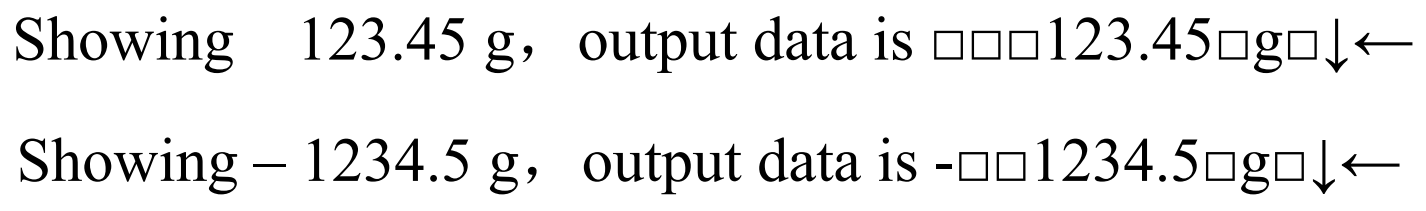
\includegraphics[scale=0.5]{obrazky/příklad protokolu - váha.PNG}
%    \end{center}
%    \label{priklad}
%    \caption{Příklad jak jsou data z displeje zapsány v datovém formátu \cite{vaha_datasheed}}
%\end{figure}



%Výstup reprezentovaný jako kod ASCII

%kombinace /r/n se vy uživa u WIndowsu k odřadkování pro 


%Vstupním portem je USB (viz. kapitola č. x), kdy piny

\section{Displej}
Další komponentou je displej, který je připojen k mikrokontroléru a zobrazuje název aktuálně měřeného destilátu, zůstatkový objem kapaliny v láhvi, maximální objem láhve, procento alkoholu měřeného destilátu a jeho obrázek pro případ, že by výrobce změnil tvar lahve, ale EAN kód by zůstal stejný.

\subsection{Požadavky na displej}
Hlavní požadavky na displej jsou:
\begin{itemize}
    \item Dotykový displej - pro budoucí implementaci klávesnice do displeje z důvodu redukce počtu periferií a snadnějšímu uživatelskému ovládání
    \item Uhlopříčka 5 - 7 palců (12,7 - 17,78 cm) pro dobrou čitelnost
    \item Bez rámečků s montážními otvory - možnost displej uchytit k vlastnímu rámu 
\end{itemize}

\subsection{Výběr displeje}

Vybraný displej je JOY-IT RASPBERRY PI touch display 7". Jeho důležité parametry jsou v tabulce č. \ref{displeej}\\

\begin{table}[!h]
    \centering
    \begin{tabular}{|c|c|}
        \hline
        Výrobce                                                         & JOY-IT   \\ \hline
        Uhlopříčka                                                      & 7" (17,78 cm)  \\ \hline
        Rozlišení                                                        & 1024 × 600 px    \\ \hline
         Rozhraní 
            & HDMI, USB \\ \hline
        Napájení & 5 V (0,6 A) \\ \hline
        Spotřeba & 3 W \\ \hline
        Dotykový displej                                                        & Ano     \\ \hline
        Cena                                                            & 2297 Kč     \\ \hline
    \end{tabular}
    \caption{Základní parametry vybraného displeje}
    \label{displeej}
\end{table}



\begin{figure}[!h]
    \begin{center}
        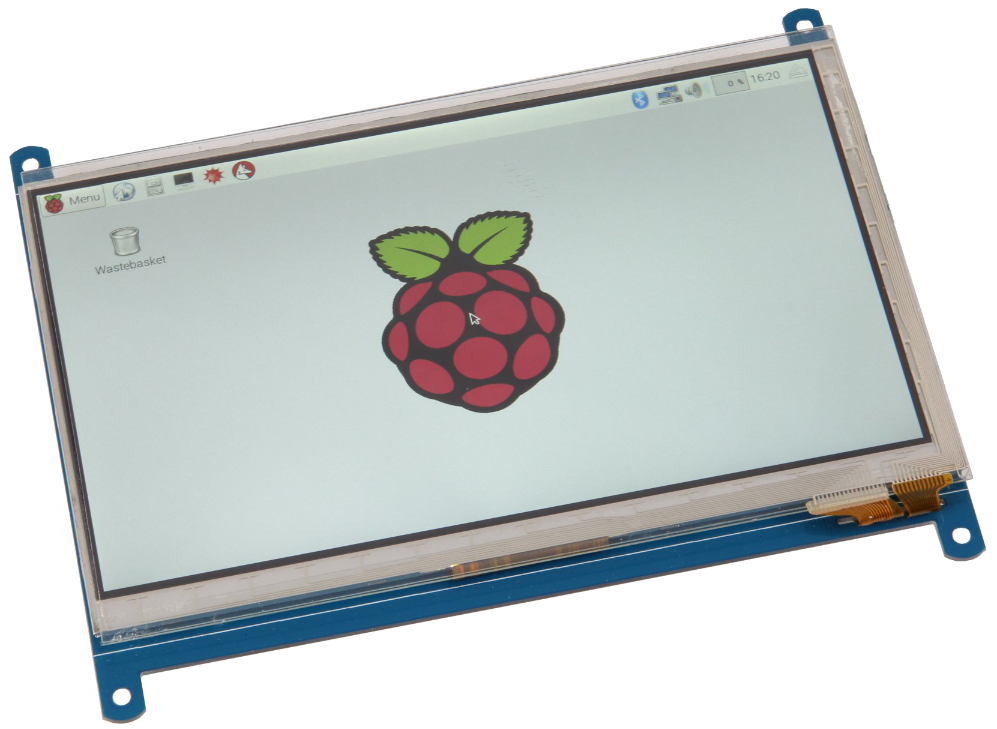
\includegraphics[scale=0.22]{obrazky/Displej.png}
    \end{center}
    \caption{Vybraný displej JOY-IT \cite{displej}}
\end{figure}

\subsection{Alternativy vybraného displeje}
Mezi alternativy můžeme zařadit:
\begin{itemize}
    \item JOY-IT RASPBERRY PI touch display 5"
    \begin{itemize}
        \item Uhlopříčka 5" (12,7 cm)
        \item Rozlišení 800x480 px
        \item Cena 1599 Kč
    \end{itemize}
    \item Raspberry Pi LCD - 7" Touchscreen
    \begin{itemize}
        \item Uhlopříčka 7" (17,78 cm)
        \item Rozlišení 800x480 px
        \item Cena 1399 Kč
        \item Horší dostupnost na českém trhu.
    \end{itemize}


    \item JOY-IT RASPBERRY PI touch display 5" - displej se liší od vybraného menší uhlopříčkou(5"), menším rozlišením(800x480) a nižší cenou(1599 Kč)
    \item Raspberry Pi LCD - 7" Touchscreen - displej se liší od vybraného menším rozlišením(800x480) a nižší cenou(1399 Kč). Jeho nevýhodou je horší dostupnost na českém trhu
\end{itemize}

%Displej je připojen k mikrokontroleru
%Displej nám bude zobrazovat data o 

\section{Čtečka čárového kódu}
Čtečka čárového kódu je zařízení, které, jak jeho název napovídá, umí číst grafický kód skládající se z černých a bílých proužků různých šířek, které reprezentují čísla splňující určitý standard pro obchodní průmysl, jako je například formát EAN. EAN (European Article Number) je mezinárodní unikátní identifikační číslo, které usnadňuje prodejcům prodej zboží. Pro český trh se běžně využívá EAN-13 (13-ti místné číslo nacházející se pod čárovým kódem). 

Čárové kódy se dělí na jednorozměrné (1D, lineární), které běžně známe z produktů v obchodech (černobílé proužky) a dvojrozměrné (2D) reprezentované jako matice bodů. Nejznámějším 2D formátem je QR (Quick Response) kod, který se využívá k rychlému placení, sdílení URL adres, připojení k internetu, atd. V praxi jsou 1D kódy, uloženy v databázi obchodu, ke kterému je přiřazen název a cena produktu.
%Čtečka čárového kódu je zařízení, které, jak jeho název napovídá, umí číst kód skládající se z černých proužků různých délek \cite{carovy_kod}, které reprezentují čísla splňující EAN standard.
%zdroj1: https://pageloot.com/cs/carovy-kod/jak-funguje-skener-carovych-kodu/
%zdroj2: https://cs.wikipedia.org/wiki/%C4%8Cte%C4%8Dka_%C4%8D%C3%A1rov%C3%A9ho_k%C3%B3du

%EAN (European Article Number) je mezinárodní unikátní identifikační číslo, které usnadňuje prodejcům prodej zboží. Pro český trh se běžně využívá EAN-13 (13-ti místné číslo nacházející se nad čárovým kódem) \cite{EAN}
%zdroj: https://cs.wikipedia.org/wiki/European_Article_Number

%V praxi je toto číslo uloženo v databázi obchodu, které je spojeno s název produktu a jeho cenou. Po načtení čárového kódu. %Po načtení čárového kódu

%V praxi je toto číslo uloženo v databázi obchodu, ke kterému je přiřazen název a cena produktu.

%Každé zboží se dá lehce indetifikovat pomocí

%V této sekci se nebudeme zabývat, jakým způsobem jsou čísla kódována do této podoby, ale jakým způsobem lze tyto čárové kódy číst.

Čárový kód se skládá z ochranných znaků „start“ a „stop“, ze středového dělícího znaku a z datových znaků, které reprezentují jednotlivé číslice. Formát EAN‑13 konkrétně určuje, že první tři číslice (tzv. prefix) značí zemi nebo region registrace, následujících šest jich slouží k identifikaci výrobce a dalších pět k rozlišení konkrétního produktu. Poslední třináctá číslice má kontrolní charakter. Vypočteme ji tak, že od konce kódu sčítáme číslice (kontrolní číslici ignorujeme) na lichých pozicích (1., 3., 5. atd.). Získaný součet vynásobíme trojkou, potom přičteme součet číslic, které leží na sudých pozicích. Výsledné číslo odečteme od nejbližšího vyššího násobku deseti a takto získaný rozdíl je kontrolní číslice. Tento postup pomáhá ověřit správnost EAN‑13 a minimalizuje chyby při skenování. [zdroj1][zdroj2]
%Zdroj1: https://is.ambis.cz/th/jmeqf/BP_Carove_kody_MMachan_3BK_IT.pdf
%Zdroj2: https://www.vut.cz/www_base/zav_prace_soubor_verejne.php?file_id=16877

\begin{figure}[!h]
    \begin{center}
        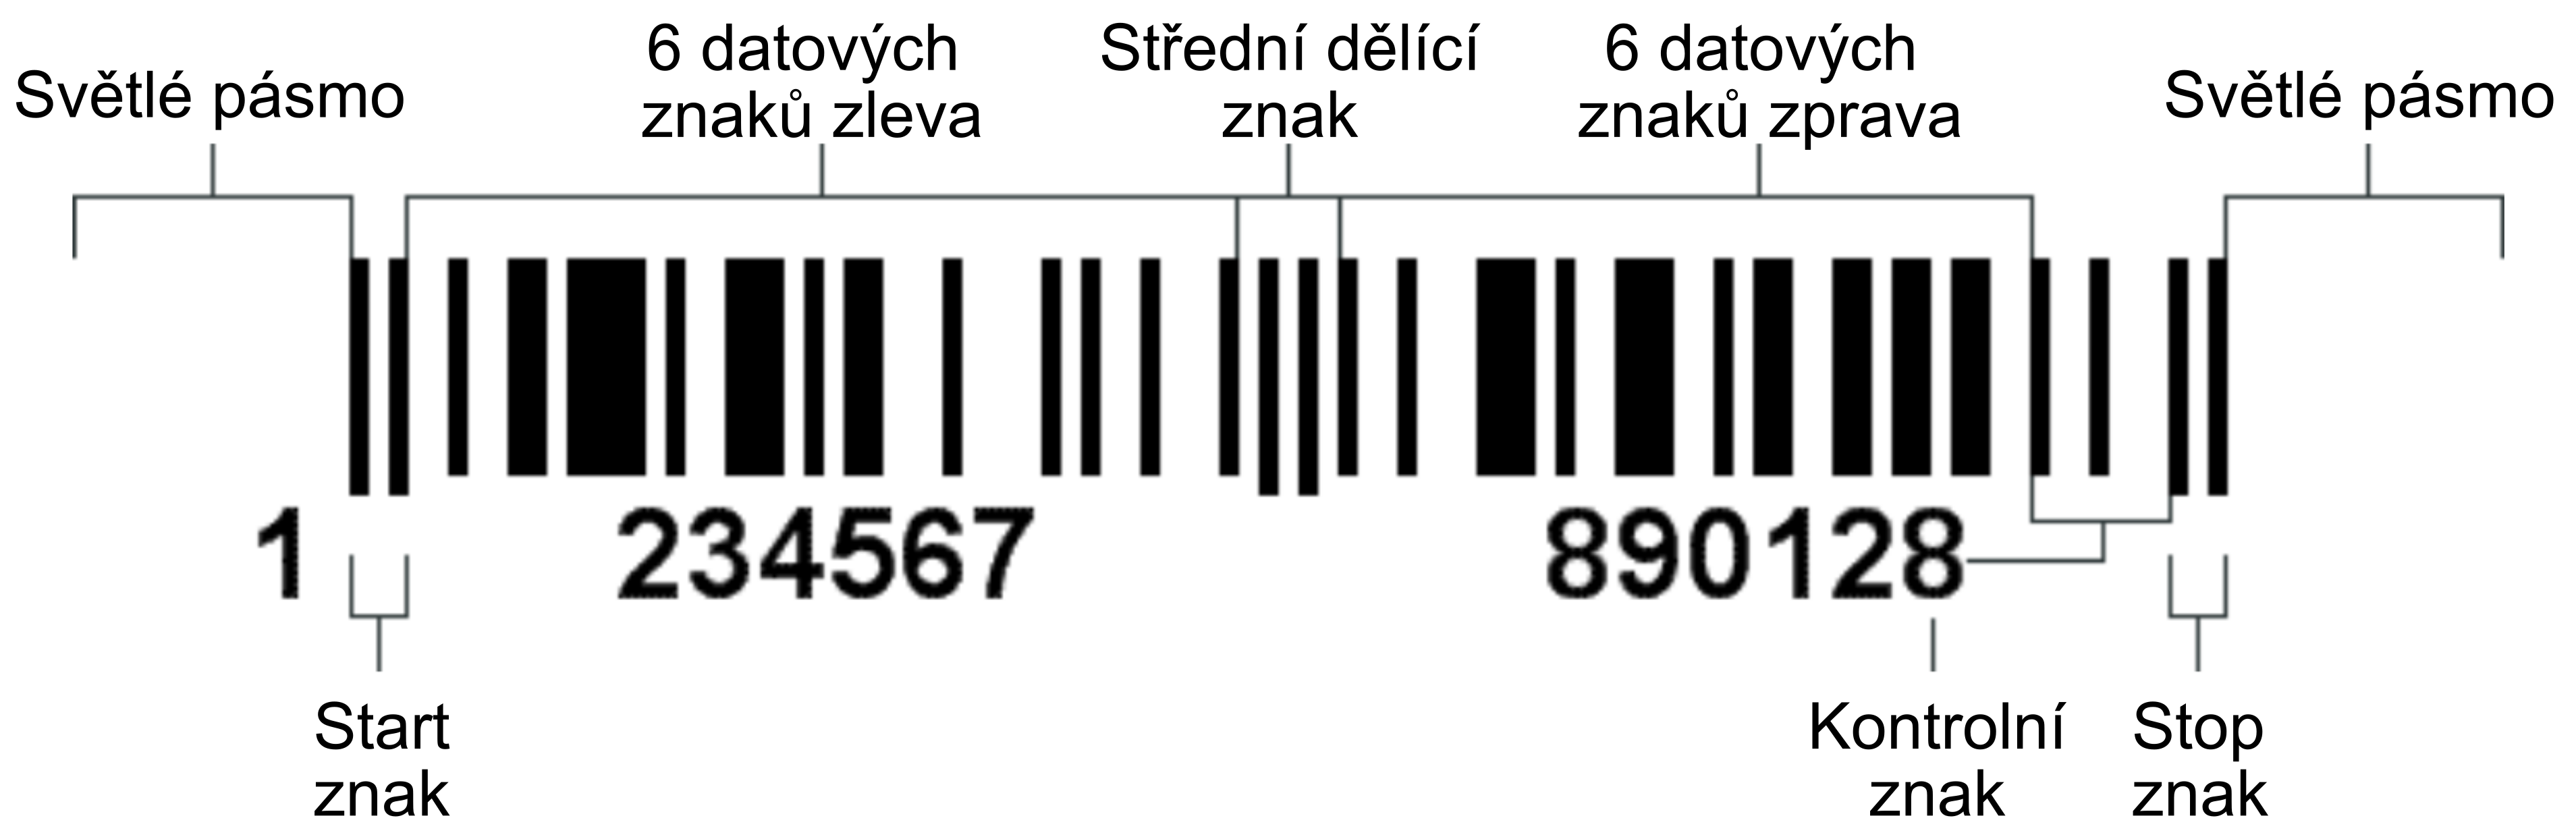
\includegraphics[scale=0.15]{obrazky/čárový kód.png} %0.5
    \end{center}
    \caption{Ukázka čárového kódu EAN-13.}
    \label{čárový kod}
\end{figure}





\subsection{Požadavky na čtečku čárového kódu}
Na trhu existuje celá řada čteček lišících se přesností, způsobem implementace a velikostí. Pro navrhovaný systém je vyžadována čtečka bez ochranného krytu s montážními otvory nebo s dostatečným prostorem pro jejich vyvrtání, aby čtečku bylo možné integrovat do vlastní konstrukce (krabičky) společně se všemi dalšími komponenty. Přednost se dává technologii CCD nebo kamerovému snímači díky vyšší mechanické odolnosti (např. při pádu) a lepší čitelnosti částečně poškozených kódů.
V poslední řadě je nutné, aby čtečka zvládala číst EAN-13 a méně často používaný EAN-8.

%dodelat zde tabulku: technologie: Kamerove (cmos), typ kodu: 1D, 2D, rychlost čtení, proudový odběr


%Na trhu je dostupných více druhů senzorů, které se liší požadavky na přesnost, druh implementace, velikostí atd. Velikost se požaduje menší bez ochranné krabičky pro budoucí uchycení do navrhnuté krabičky, která zastřeší všechny komponenty systému na jednom místě. včetně montážních otvorů nebo dostatečného prostoru pro jejich vyvrtání. Preferovanou technologií je CCD nebo CMOS z důvodu větší durability např. při pádu měřícího systému na zem a lepší čitelnosi poškozených kódů. Navíc od roku 2025 by mělo z obchodník řetězců vymizet klasické 1D čárové kódy a měli by je nahradit 2D QR kody, otázkou je zda přibude i nový formát 2D kódů na kterou budou vyvýjeny nové čtecí systémy

%Požaduje se komunikační rozhraní, nejlépe USB nebo UART pro odesílání a přijímání dat ze čtečky. Datový formát nejlépe ASCII, stejně jako u vybrané váhy, pro jeho jednoduché zpracování.

%Komunikační rozhraní čtečky se požaduje UART nebo USB s možností povolení virtuálního seriového portu pro komunikaci s mikrokontrolérem - označováno USB VCom.

%Další požadavek spočívá v tom, aby čtečka byla schopna číst standard EAN-13, který je běžně používán v České republice, a také EAN-8, s nímž se lze výjimečně setkat.
\subsection{Vybraná čtečka čárového kódu}

%Vybraná čtečka je GM65 od společnosti KROW, využívající CMOS technologie, obrázek č.\ref{gm65}.
%Čtečka disponuje UART a USB VCom. Kompletní specifikace je obsažena v dokumentaci.\cite{scaner}
%Datový formát pro seriovou komuniaci čtečky je stejný jak u vybrané váhy[xx] i zde chybý ověřovací bit, který bude ošetřen softwarově

%Z důvodu technologického pokroku a podle výše zmíněných parametrů jsem byl schopen najít pouze CMOS čtečky, proto tedy vybraná čtečka je GM65....

S ohledem na výše uvedené požadavky byla vybrána kamerová čtečka KROW GM65, využívající optických snímačů CMOS (viz obrázek č.\ref{gm65}) a LED diody pro nasvícení čárového kódu v hůře osvětleném prostředí. Čtečka nabízí komunikační rozhraní UART a USB. Datový formát pro sériovou komunikaci je shodný s vybranou váhou [\ref{datový paket váhy}].
%Podobně jako u váhy chybí ověřovací bit, který bude řešen softwarově. Podrobné technické specifikace čtečky jsou uvedeny v její dokumentaci.

\begin{table}[!h]
    \centering
    \begin{tabular}{|c|c|}
        \hline
        Výrobce                & KROW             \\ \hline
        Model                  & GM65             \\ \hline
        Typ                    & Kamerová čtečka  \\ \hline
        Čtecí vzdálenost \tablefootnote{Pro standart EAN-13 s šířkou kódu 35,6 mm při intenzitě osvětlení 250 lux}       & 4 - 25 cm            \\ \hline
        Rozhraní & HDMI, USB \\ \hline
        Napájení               & 5 V (až 160 mA)  \\ \hline
        Spotřeba               & 0,8 W            \\ \hline
        Rychlost čtení         & 0,1 s            \\ \hline
        Cena                   & 992 Kč           \\ \hline
    \end{tabular}
    \caption{Základní parametry vybraného displeje}
    \label{displeej}
\end{table}


\begin{figure}[!h]
    \begin{center}
        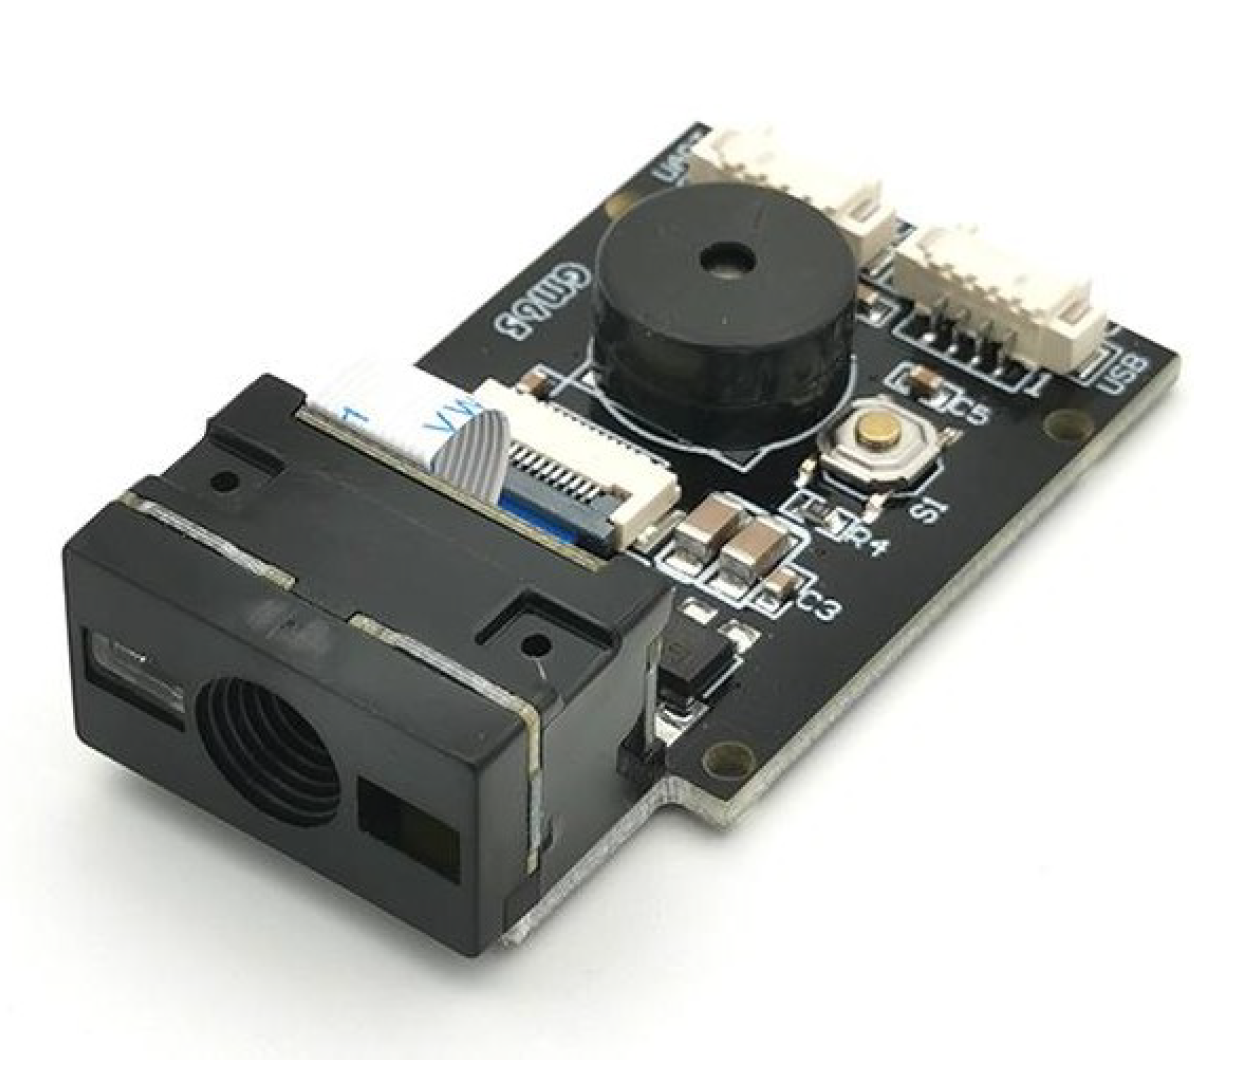
\includegraphics[scale=0.25]{obrazky/gm65.PNG} %0.5
    \end{center}
    \caption{Vybraná čtečka čárového kódu KROW GM65 \cite{scaner}}
    \label{gm65}
\end{figure}

%Toto níže je blbost
%\begin{table} [!h]
%    \centering
%    \begin{tabular}{|l|l|l|l|l|l|}
%    \hline
%         Hlavička  & Typ & Délka dat & Adresa & Data & CRC \\ \hline
%         2 B       & 1 B & 7 B       & 3    B & 1 B  & 1 B\\ \hline 
%    \end{tabular}
%    \caption{Předpis výstupních dat}
%    \label{datovy format čtečky}
%\end{table}




\subsection{Alternativy vybrané čtečky čárového kódu}
%Mezi alternativy můžeme zařadit:
%Vybrané alternativy jsou kamerové

\begin{itemize}
    \item YHDAA YHD-M800D
    \begin{itemize}
        \item Typ: Kamerový snímač
        \item Cena: 1000 Kč
        \item Rozhraní: USB
        \item Nepřehledná a nevypovídající dokumentace
    \end{itemize}
    \item WaveShare Barcode Scanner
    \begin{itemize}
        \item Typ: Kamerový snímač
        \item Cena: 1318 Kč
        \item Rozhraní: USB, UART
    \end{itemize}
\end{itemize}


%\begin{itemize}
  %  \item YHDAA YHD-M800D - kamerová čtečka, cenově stejně dostupné(1000 Kč) jak vybraná čtečka, integrovaný USB port, nepřehledná a nevypovídající dokumentace 
 %   \item WaveShare Barcode Scanner - kamerová čtečka, dražší než vybraná čtečka(1318 Kč), integrovaný sériový port micro USB a UART
%\end{itemize}

\section{Modul s výpočetní jednotkou} %Mikrokontroler
%Výpočetní modul / Modul s výpočetní jednotkou / Řídící jednotka / Výpočetní jednotka

Modul s výpočetní jednotkou je samostatná hardwarová součást (obvykle deska plošných spojů osazená procesorem, pamětí a potřebnými rozhraními), která ve větším elektronickém či řídicím systému zajišťuje hlavní výpočetní výkon. Často pracuje v kombinaci s jinými moduly – sběrnicovými, vstupními (senzory, klávesnice), výstupními (displeje, motory) nebo dalšími výpočetními jednotkami. Mezi běžné představitele těchto výpočetních jednotek patří:
\begin{itemize}
    \item Mikrokontrolery (Jednočipové PC, MCU): Jsou to systémy na jednom čipu, které integrují procesor, paměť flash a RAM, A/D převodník, oscilátor (hodiny) a I/O porty. Běžně se využívají v real-time aplikacích, jež nevyžadují vysoký výpočetní výkon.
    \item Jednodeskové počítače (SBC, mikropočítače): Vyšší stupeň integrace oproti mikrokontrolérům. Jde o plnohodnotné počítače na jedné desce. Obvykle běží pod operačním systémem a nabízejí více periferií, což je činí vhodnými pro komplexní a výpočetně náročnější úlohy.
\end{itemize}


%Mikrokontroler jinak označovaný jednočipový počítač je integrovaný obvod
%Mikrokontrolér nebo také jednočipový počítač je integrovaný obvod obsahující kompletní mikropočítač. Jednočipové počítače se vyznačují velkou spolehlivostí a kompaktností, proto jsou určeny především pro jednoúčelové aplikace. Mikrokontroléry jsou často používány v embedded systémech, jako jsou například řídicí systémy, regulátory, senzory a další aplikace, kde je potřeba rychle a spolehlivě zpracovávat data. V praxi si můžeme pod takovou řídící jednotkou představit např. PLC (Programovatelný automat)
%[zdroj]
%Na bakalařku překopat...je to opsaný
%https://sk.wikipedia.org/wiki/Mikrokontrol%C3%A9r
%https://cs.wikipedia.org/wiki/Jedno%C4%8Dipov%C3%BD_po%C4%8D%C3%ADta%C4%8D

\subsection{Požadavky na modul s výpočetní jednotkou} %Požadavky na řídící jednotku / výpočetní modul
%napájení
%OS(bez os nepojede databaze atd) a grafická čip, hdmi,  pro vývoj GUI
%Jednodeskotopový PC skrz chod pythonu a Tkinter, ten na mikrokontroleru nerozjedu skrz malou pamět a výkon a na MikroPython nic takového nebude. Dále mikrokontorler nemá SD slot pro ukládání databáze
%V mobilu mam napsany od petyho proč nevybrat to a tam a nejaky popis k mikrokontrolerum

%

Hlavním z požadavků je snadná realizovatelnost firmware s integrovaným grafickým uživatelským rozhraním(GUI) ovládaného dotykovým displejem. Pro takové účely je vhodné použít vysokoúrovňový programovací jazyk, např. Python, který nabízí široký výběr knihoven a nástrojů, které ulehčují a zrychlují vývoj samotného firmware, na druhou stranu je nutné přihlédnout na dostačující výkon a operační paměť(RAM) řídící jednotky. Vývoj GUI a práce s databází obnáší zpravidla přítomnost OS už jen z důvodu zabudovaných grafických ovladačů pro komunikaci s displejem, správu paměti nebo využití grafických knihoven, které je pro svoji funkčnost OS vyžadují, proto využiji nenáročné distribuce linuxu, která je oproti konkurenčním OS výkonově i paměťově nenáročná.
%Z důvodu volby vysokoúrovňového programovacího jazyku, GUI a využití databáze je nutné, aby firmware běžel na OS.
%Z důvodu minimální výkonové a paměťové náročnosti poběží řídící jednotka na nenáročné distribuci Linuxu. Pro takový účely se hodí libovolná distribuce linuxu, která je hojně využívána u jednodeskových počítačů.

Další požadavky:
\begin{itemize}
    \item Výkon a paměť: 
        \begin{itemize}
            \item Dvou a více jádrový procesor pro paralelní chod GUI a stavového automatu pro zpracování dat ze čtečky čárového kódu a váhy. 
            \item Minimální velikost RAM paměti 2 GB, optimálně 4-8 GB pro plynulý chod GUI a OS.
        \end{itemize}
    \item Periferie:
        \begin{itemize}
            \item 3x USB-A(optimálně verze 3.0) pro čtečku čárového kódu, váhu a napájení displeje. Výstupní proud alespoň 0,6 A 
            \item 1x HDMI nebo Micro HDMI pro dotykový displej
            \item slot na SD kartu na které budou uložena veškerá data databáze zmíněná v kapitole č. 5.3, operační systém a samotný firmware. Velikost SD karty alespoň 32 GB[zdroj1] pro plynulý chod OS  
            %pro optimální rychlost čtení a zápisu [zdroj1][zdroj2]. %Například pro Rasbian OS (OS jednodeskových počítačů(SBC) raspberry pi) je doporučovaná velikost minimálně 4 GB[Zdroj1]
            %Zdroj1 : https://www.raspberrypi.com/documentation/computers/getting-started.html
            %Zdroj2 : https://www.raspberrypi.com/documentation/accessories/sd-cards.html
            \item Řídící jednotka musí zvládnout poskytnout dle vybraných komponent, alespoň 0,7 A při 5 V, optimálně 1,2 A, pro případ rozšíření systému o další komponenty.
            %\item Alespoň jeden GPIO pro ovládání pípáku
        \end{itemize}
    \item Integrovaný Wi-Fi modul: Do budoucna je cílem bezdrátová konektivita s měřícím systémem pomocí mobilní aplikace nebo připojení k ERP systémům
    %\item napájení/odběr/příkon/spotřeba: ...
    %Výstupní proud 0,6 A (USB): Výkonově nejnáročnější komponentou připojené k řídící jednotce bude displej[] s proudovým odběr 0,6 A při 5 V. (Do budoucna bude měřicí systém bude obsahovat baterii, který může napájet jednotlivé komponenty.) Pro provoz displeje, který je proudově nejnáročnější je nutné, aby USB porty dokázaly poskytnout minimálně 0,6 A při 5 V. Řídící jednotka musí zvládnout poskytnout dle vybraných komponent, alespoň 0,7 A při 5 V, optimálně 1,2 A, pro případ rozšíření systému o další komponentu.
\end{itemize}

%Nevybírat model s konrétní velikost ram, ale určit více velikostí a pak podle toho dát rozsah ceny
\subsection{Vybraný modul s výpočetní jednotkou}
Na základě výše zmíněných požadavků byl vybrán jednodeskový počítač Raspberry Pi 4 ve verzi s 4 GB operační paměti. Kategorii mikrokontrolérů jsem úplně vynechal z důvodu nedostatečného výkonu a operační paměti pro chod OS s GUI aplikací a absence integrovaných periférií jako USB nebo HDMI. 

Mezi klíčové výhody Raspberry Pi patří široká komunita, kvalitní podpora i bohatá škála dokumentace a knihoven. Další z výhod je rozumný poměr cena výkon a spolehlivost. Základní technické parametry jsou přehledně uvedeny v tabulce č. \ref{raspbericko_spec}, zatímco kompletní specifikace lze nalézt v příslušné dokumentaci. \cite{Raspberry pi}

%Vyrobce
%Model
%Procesor
%RAM
%Rozhraní 2x USB 2.0, 2x USB 3.0, 2x HDMI 1.4 (asi)
%Napájení 5V DC
%Spotřeba 4 - 7 W
%Dále obsahuje: Wi-Fi/BT modul, SD slot, 3,5 mm Jack


\begin{table}[!h]
    \centering
    \begin{tabular}{|c|c|}
        \hline
        Výrobce                                                         & Raspberry Pi Foundation   \\ \hline
        Model                                                           & Raspberry Pi 4  \\ \hline
        %\begin{tabular}[c]{@{}c@{}}Komunikační\\ protokol\end{tabular}  & UART   \\ \hline
        CPU & \begin{tabular}[c]{@{}c@{}}1.5GHz čtyřjádrový \\ ARM Cortex-A72\end{tabular} \\ \hline
        GPU & VideoCore VI 500 MHz \\ \hline
        RAM & 4 GB \\ \hline
        Periferie & \begin{tabular}[c]{@{}c@{}} 2x USB-A 3.0 \\ 2x USB-A 2.0 \\ 1x USB-C (napájení) \\ 2x microHDMI 2.0 \\ 1x Gigabit Ethernet \\ 40x GPIO \end{tabular} \\ \hline
        Napájení                                                        & 5 V DC (až 3 A)   \\ \hline
        Spotřeba                                                        & 3 - 7 W     \\ \hline
        Dale obsahuje & \begin{tabular}[c]{@{}c@{}} Wi-Fi/BT modul \\ SD slot \end{tabular} \\ \hline
        Cena                                                            & 1987 Kč     \\ \hline
    \end{tabular}
    \label{raspbericko_spec}
    \caption{Základní parametry Raspberry Pi 4 \cite{Raspberry pi}}
\end{table}

%Hlavní nevýhodou je pořizovací cena 1479 Kč a vyšší spotřeba energie v rozmezí 3 - 7 W. Kompletní specifikace se nachází v dokumentaci výrobce.[2]



%Vybraný mikrokontroler byl Raspberry PI 4, který dokáže pokrýt veškeré požadavky na měřicí systém. Konkrétně se jedná o model B s 4 GB operační paměti. Zde jsou zmíněné požadavky na mikrokontrolér:

%\begin{itemize}
%    \item Dostatečný počet portů pro připojení všech modulů.
%    \item Integrovaná čtečka SD karty pro ukládání databáze
%    \item Dostatečný výkon pro chod GUI aplikací. Do budoucna je v plánu implementovat dotykový displej, na kterém budou veškeré informace pěkně přehledné díky grafickému rozhraní
%    \item Integrovaný čip pro bezdrátovou konektivitu. Do budoucna možnost vývoje mobilní aplikace k vyvíjenému systému nebo bezdrátové připojení k ERP systémům.
%    \item
%    \item Hlavní z požadavků je snadná realizovatelnost firmware s integrovaným grafickým uživatelským rozhraním pro ovládání dotykového displeje. Pro takový účely je vhodné použít programovací jazyk Python, který nabízí širší výběr knihoven a nástrojů, které ulehčují a zrychlují vývoj samotného firmware.
%
%    \item
%\end{itemize}
%Dost požadavků je nad rámec bakalářské práce, ale pro budoucí inovaci systému nemusíme měnit mikrokontrolér a realizovat znovu už fungující HW kompatibilitu mezi komponenty a vyvíjet SW vybavení.

%Jedinou nevýhodou je vysoká pořizovací cena.

\begin{figure}[!h]
    \begin{center}
        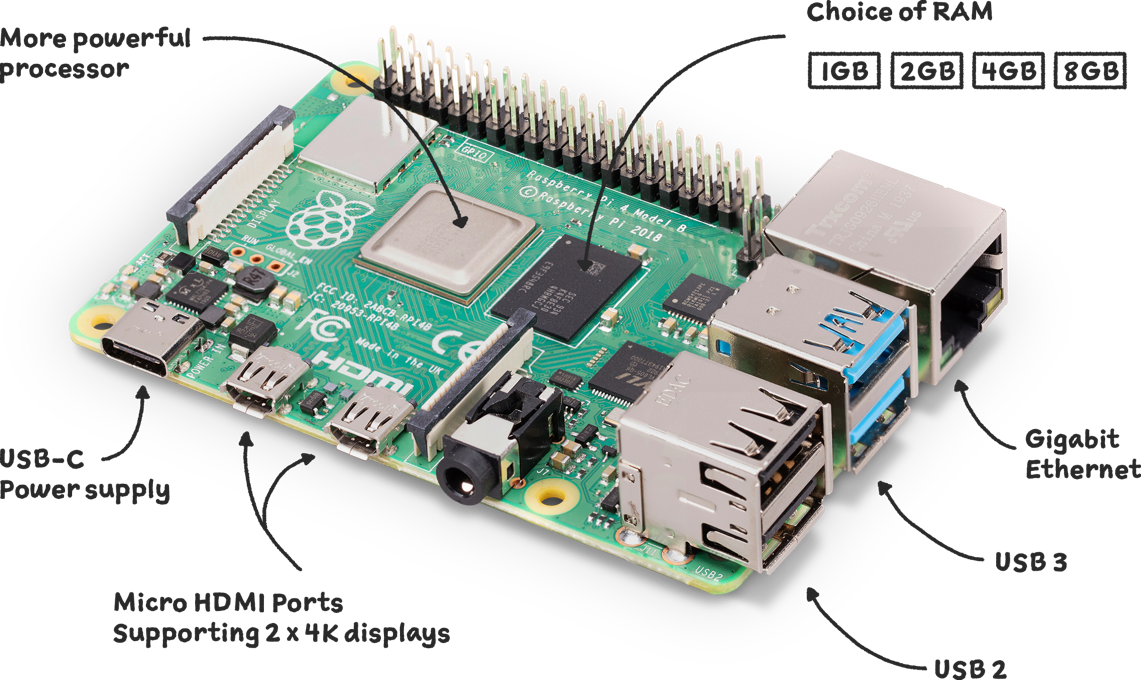
\includegraphics[scale=0.3]{obrazky/raspberry-pi-4.png}
    \end{center}
    \caption{Vybraný jednodeskový PC Raspberry Pi 4 \cite{malina_obr}}
    %\label{gm65}
\end{figure}

\subsection{Alternativy vybraného modulu s výpočetní jednotkou}

%Raspberry piko
%Arduino Uno
%Esp 32 (SoC/mikrokontroler + WIFI/BT)
%Acemagic T8-PRO N5105 (8+0) Silver (Přebustěny jednodeskový pc / mini PC)

\begin{itemize}
    \item ESP32 (MCU)
        \begin{itemize}
            \item Zlomová cena - 200 Kč
            \item Absence debuggeru
            \item ...
        \end{itemize}
    \item Banana Pi M5 (Druhá nejlepší volba)
        \begin{itemize}
            \item[$-$] "Čínská" kopie raspberry pi 4
            \item[$+$] Výkonnější procesor - Cortex-A55 (4 jádra, 2 GHz)
            \item[$+$] Integrované uložiště eMMC (rychlejší než SD karta)
            \item[$-$] Horší dostupnost v lokálních e-shopech (často nutný dovoz)
            \item[$-$] Menší uživatelská základna - méně zdrojů, tutoriálů a komunitních projektů
            \item[$+$] 2000 Kč
        \end{itemize}
    \item Odroid XU4
        \begin{itemize}
            \item[$-$] Absence Wi-Fi modulu
            \item[$-$] Pouze 2 GB RAM
            \item[+] eMMC modul
            \item[$+$] Komunita kolem Hardkernel Odroidů je relativně aktivní
            \item[$-$] Stále menší komunita než u Raspberry
        \end{itemize}
    %- Jen 2 GB RAM. Nemá integrovaný Wi-Fi modul, nutnost připojit externě.
    \item NVIDIA Jetson Nano 
        \begin{itemize}
            \item[$-$] Cenově náročný - 8000 Kč
            \item[$+$] Zbytečně vysoký grafický výkon. Vhodnější spíše pro strojové učení a práci s AI.
            \item[$-$] Absence Wi-Fi modulu (možnost externího připojení)
            \item[$-$] Vyšší spotřeba 7 - 24 W
        \end{itemize}
    \item Recyberry Asus Tinker Board S. 
        \begin{itemize}
            \item[$-$] Aktuálně nedostupný na českém trhu%Horší dostupnost v lokálních e-shopech
            \item[$-$] Operační paměť max. 2 GB
            \item[$-$] Pouze USB 2.0 (10x pomalejší než USB 3.0 %[zdroj: to co useriove komunikace])
            \item[+] Integrovaný eMMC (rychlejší načtení OS)
        \end{itemize}
    %\item Recyberry Asus Tinker Board 2S - Vyší napájecí napětí 12-19 V, 
    %\item Arduino Portenta X8 - Nemá nativní HDMI port, ale zde využít USB-C konektoru jako Displey Port a pro ostatní USB porty použít USB rozbočovač
\end{itemize}



%Rozhodoval jsem se mezi dalšími dvoumi 







%proč malinu:
%
%-graficky čip pro dotykovy displej, 
%
%-wifi/BT čip pro budouci mobilni aplikaci, 
%
%-možnost vývoje GUI (python, CS) bezne mikrokontrole funguje jen na C/C++ asi,
%
%-rozumně velké uložiště pro ("GUI aplikaci" spíš RAM) databázi, která se časem bude rozšiřovat nevim jestli by arduino to pojmulo, ale určitě arduino nepojme databází obrázků, jednotlivých destilátů
%%https://www.dps-az.cz/clanky/id:6173/uvod-do-embedded-systemu
\chapter{Zprovoznění jednotlivých komponent}
\label{Zprovoznění jednotlivých komponent}
Jednotlivé komponenty jsou připojeny k mikrokontroléru podle obrázku č. \ref{blokove_schema}. Displej a klávesnici stačí jen připojit, proto je nebudu v rámci této kapitoly více rozebírat.

\section{Ověření přesnosti váhy}

Před použitím samotné váhy jsem ověřil, zda její přesnost odpovídá parametrům stanoveným výrobcem z důvodu, že váha není certifikovaná. Ověření probíhá pomocí druhé váhy nebo kalibrovaného závaží o jednu třídy přesnosti výše. Pro váhu integrovanou do měřícího systému GG xxx je třída přesnosti III, proto je nutné volit váhu s třídou přesnosti II dle normy OIML R 76 nebo kalibrované závaží s třídou přesnosti M1 dle normy OIML R 111. Pro ověření přesnosti byla použita váha Kern PCB-2500-2 s padesátkrát vyšší přesností: 0,01 g a váživostí 2,5 kg. Obě váhy byly před použitím kalibrovány a použity v laboratorním prostředí s teplotou 20,4 °C a vlhkostí 28,7 \%, které odpovídají požadavkům obou výrobců vah pro přesná měření. Z tabulky č. \ref{tab:vahy} je vidět, že váha G\&G-3000 měří s požadovanou přesností 0,5 g. %a spadá tak do třídy přesnosti III.




%\begin{table}
%    \centering
%    \begin{tabular}{|c|c|}
%    \hline
%         \begin{tabular}[c]{@{}c@{}} Kern PCB-2500-2 \\ (g) \end{tabular} & \begin{tabular}[c]{@{}c@{}} G\&G E3000 \\ (g) \end{tabular}\\ \hline
%         20,00 & 20,0\\ \hline
%         200,00&200,0 \\ \hline
%         400,00&400,0 \\ \hline
%         600,00 & 600,0 \\ \hline
%         800,00&800,0 \\ \hline
%         1000,00&1000,0 \\ \hline
%         1200,00&1200,0 \\ \hline
%         1400,00&1400,0 \\ \hline
%         1600,00&1600,0 \\ \hline
%         1800,00&1800,0 \\ \hline
%         2000,00&2000,0 \\ \hline
%         2200,00&2200,0 \\ \hline
%    \end{tabular}
%    \caption{Ověření přesnosti váhy G\&G E3000}
%    \label{tab:vahy}
%\end{table}

\begin{figure}[H]
    \begin{center}
        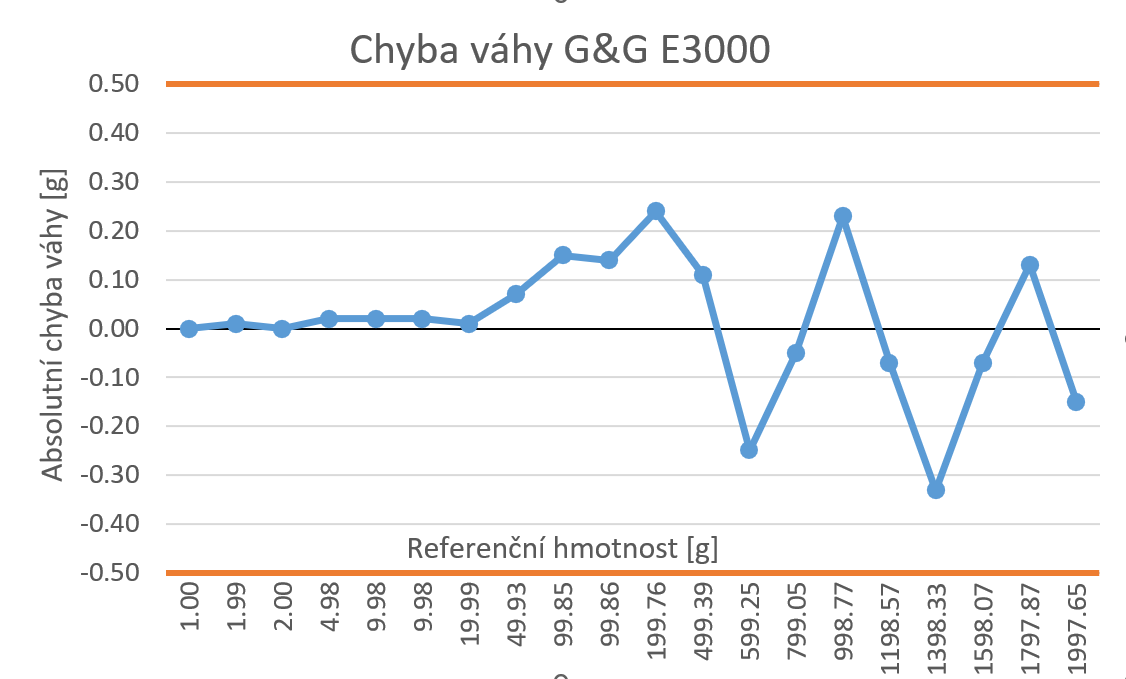
\includegraphics[scale=0.6]{obrazky/mereni.PNG}
    \end{center}
    \caption{Nalevo Kern PCB-2500-2, napravo G\&G E3000}
    \label{adapter}
\end{figure}

\begin{figure}[H]
    \begin{center}
        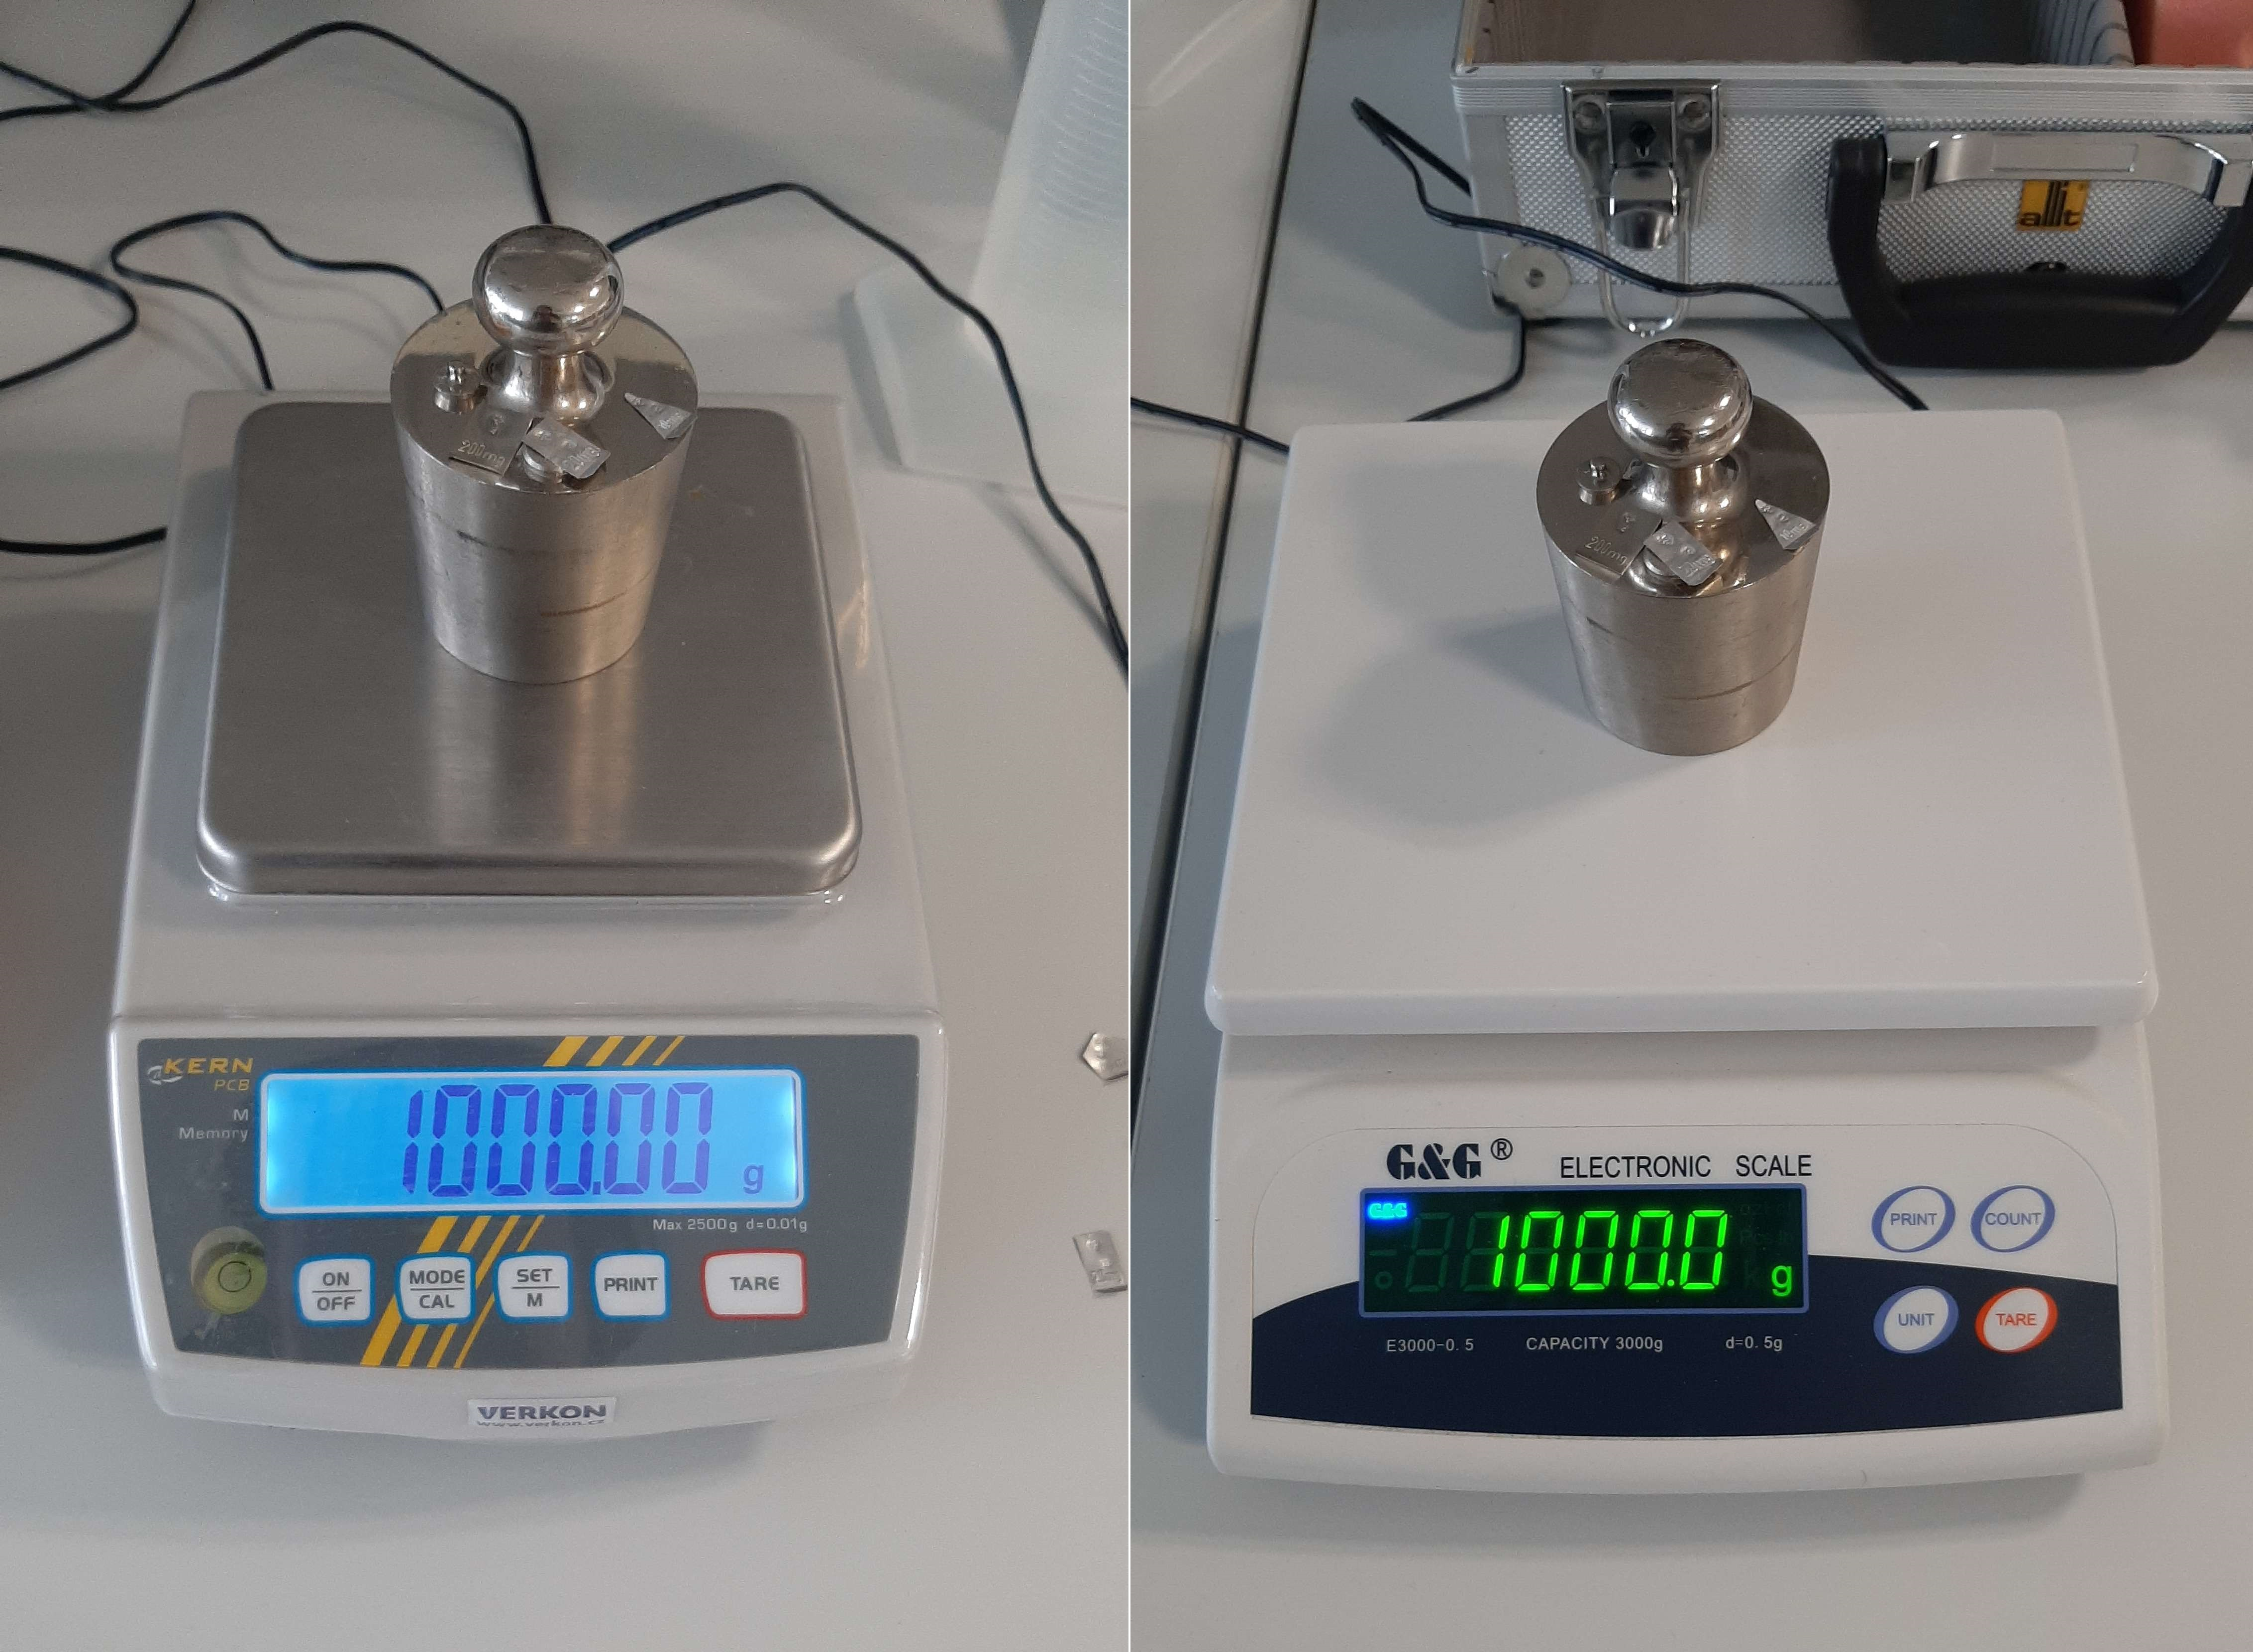
\includegraphics[scale=0.1]{obrazky/vahy.jpg}
    \end{center}
    \caption{Nalevo Kern PCB-2500-2, napravo G\&G E3000}
    \label{adapter}
\end{figure}

\section{Zprovoznění váhy}

Komunikační rozhraní váhy je RS-232, který nejsme schopni připojit na mikrokontrolér z důvodu absence totožného rozhraní. V takovém případě použijeme adaptér z RS-232 na USB. Použitý adaptér je ADS-50 USB - serial, který je součástí balení váhy. (obrázek č.\ref{adapter})

\begin{figure}[H]
    \begin{center}
        \includegraphics[scale=0.06]{obrazky/ADS-50 USB - serial adapter.png}
    \end{center}
    \caption{Adaptér USB - serial AXAGO ADS-50}
    \label{adapter}
\end{figure}

Propojení kabelu ADS-50 s váhou není možné z důvodu, že kabel není křížený, jinak zvaný "null modem" kabel. To znamená, že vysílací piny(Tx) jsou navzájem propojené a to samé přijímací piny(Rx). Aby komunikace mohla fungovat je nutné propojit Tx s Rx. Tato podmínka komunikace je zmíněná v dokumentaci váhy[x]. Výrobce váhy z tohoto důvodu k balení přidal kříženou redukci DB9(samice) - DB9(samice), která slouží současně k monitorování stavu jednotlivých pinů díky přídavným konektorům pro připojení např. osciloskopu. Dále výrobce přidal redukci DB9(samec) - DB9(samec) pro propojení křížené redukce s váhou(samice). Zapojení je možné vidět na obrázku č.\ref{propojení váhy v1}. Toto zapojení není praktické pokud nechceme diagnostikovat komunikaci, proto je možností koupit přímo křížený kabel nebo kříženou redukci, která vychází 5x levněji. Na obrázku č.\ref{propojení váhy v2} je výsledné řešení propojení váhy s mikrokontrolerem pomocí křížené redukce DB9(samec) - DB9(samice).

\begin{figure}[H]
    \begin{center}
        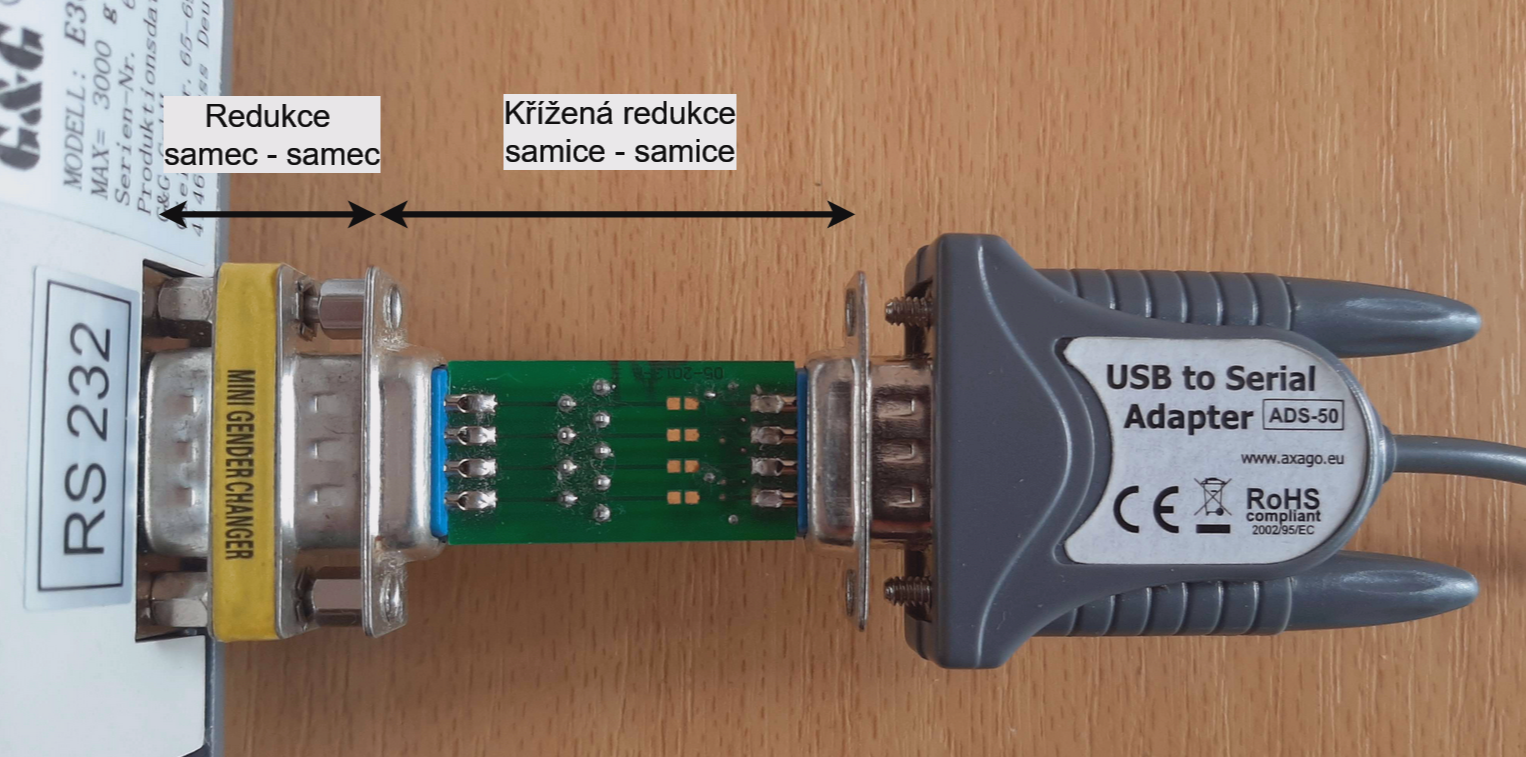
\includegraphics[scale=0.27]{obrazky/zapojeni_vahy_v1 - popis.png}
    \end{center}
    \caption{Propojení váhy s mikrokontrolerem pomocí komponent dodané výrobcem váhy}
    \label{propojení váhy v1}
\end{figure}

\begin{figure}[H]
    \begin{center}
        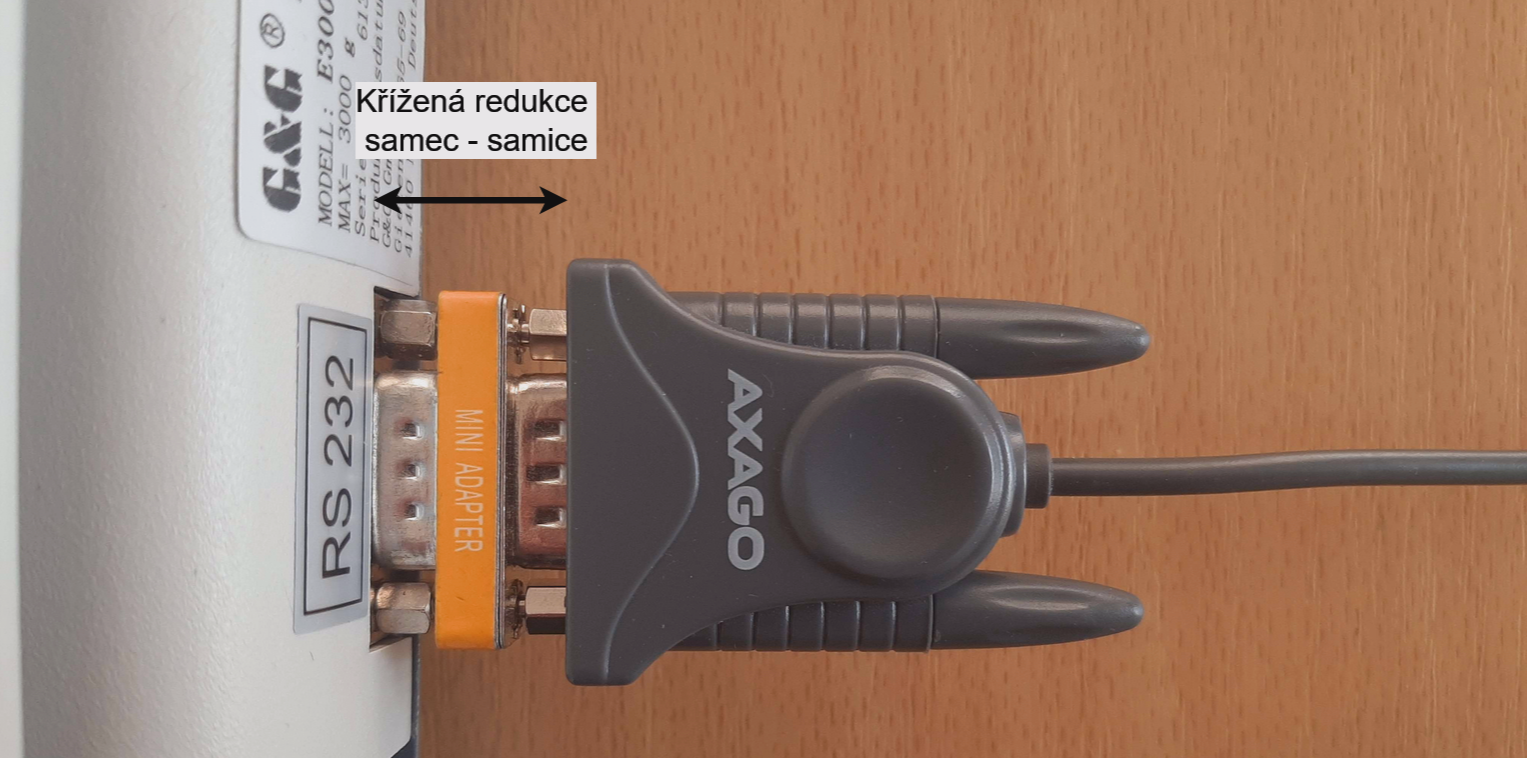
\includegraphics[scale=0.27]{obrazky/zapojeni_vahy_v2 - popis.png}
    \end{center}
    \caption{Výsledné propojení váhy s mikrokontrolerem}
    \label{propojení váhy v2}
\end{figure}

Dalším krokem je nastavení parametrů sériové komunikace podle manuálu váhy\cite{vaha_datasheed}. Komunikace byla testována pomocí osciloskopu s funkcí čtení UART protokolu a windows nástroje PuTTY, který přijímal/odesílal data po sériové lince. 
Na obrázku č. \ref{putty} je nastavení parametrů v PuTTY a na obrázku č.\ref{puttyyyy} je vidět, že váha nám na výstup konzole PuTTY posílá aktuální naměřená data.


\begin{figure}[H]
    \begin{center}
        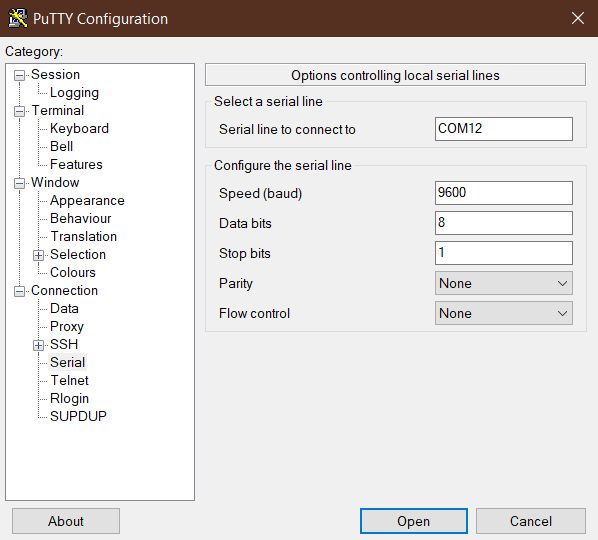
\includegraphics[scale=0.8]{obrazky/nastaveni putty.png}
    \end{center}
    \caption{Nastavení parametrů komunikace v PuTTY}
    \label{putty}
\end{figure}

\begin{figure}[H]
    \begin{center}
        \includegraphics[scale=0.09]{obrazky/komunikace váha putty.jpg}
    \end{center}
    \caption{Čtení sériové komunikace váhy pomocí PuTTY}
    \label{puttyyyy}
\end{figure}

Na obrázku č.\ref{osc} byl datový výstup váhy testován pomocí osciloskopu. Parametry na osciloskopu byly nastaveny obdobně jak na obrázku č.\ref{putty}

\begin{figure}[H]
    \begin{center}
        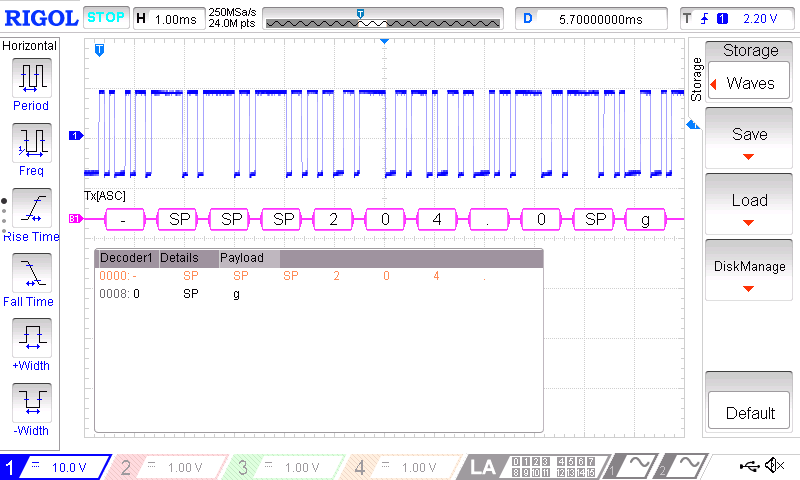
\includegraphics[scale=0.5]{obrazky/DS1Z_QuickPrint6.png}
    \end{center}
    \caption{Odchycení zprávy "-204.0 g" pomocí osciloskopu}
    \label{osc}
\end{figure}

%%%%%%%%%%%%%%%%%%%%%%%%%%%%%%%%%%%%%%%%%%%%%%%%%%%%%%%%%%%%%%%%%%%%%%%%%%%%%%%%%%%%%%%%%%%%%%%%%%%%%%%%%%%%%%%%%%%%%%%%%%%%%%%%
\section{Zprovoznění čtečky čárového kódu}
\label{zprovozeni_ctecky}
%Čtečka čárového kódu ve výchozím nastavení se chová jako klávesnice(HID KBW), aby bylo možné číst sériovou komunikaci je nutné naskenovat QR kód z manuálu\cite{scaner}, který přepíná výstup čtečky z HID KBW na virtuální sériový USB port(USB VCom).

Čtečka čárového kódu se ve výchozím nastavení chová jako klávesnice (USB HID KBW). To znamená, že pokud máme otevřený textový editor (například Word) a načteme čárový kód, data se vypíšou přímo do dokumentu, jako by byla zadána z běžné klávesnice.

Tento režim je však pro programové zpracování dat nepraktický – neumožňuje obousměrnou komunikaci, data nejsou strukturována do žádného rámce a není možné spolehlivě rozlišit začátek a konec zprávy. Výstup je navíc směrován do aktivního okna systému, což ztěžuje jeho přesné zachycení v aplikacích.

Z těchto důvodů výrobce poskytuje možnost přepnout čtečku do režimu USB VCOM (virtuální COM port). V tomto režimu čtečka emuluje sériový port přes USB, což umožňuje snadné a přesné čtení výstupu v programech jako je Python, HTerm nebo PuTTY – včetně možnosti odesílat příkazy zpět do čtečky.
\\\\
Čtečka tedy nabízí 3 komunikační rozhraní:
\begin{itemize}
    \item \textbf{UART} - Jeden z nejjednodušších sériových komunikačních protokolů, viz kapitola č. \ref{UART protokol}. Připojení k Raspberry Pi pomocí označených GPIO pinů: Tx a Rx. 
    \item \textbf{USB HID (Human Interface Device)}
    \begin{itemize}
        \item \textbf{USB HID KBW (Keyboard)} - emulace klávesnice (výchozí nastavení)
        \item \textbf{USB HID POS (Point of Sales)} - speciální protokol pro POS aplikace 
    \end{itemize}
    \item \textbf{USB VCom} - Virtuální sériový COM port, který emuluje UART komunikaci přes USB. Oproti klasickému UART rozhraní je USB VCOM stabilnější (integrovaná nízkoúrovňová CRC kontrola přenosu), jednodušší na zapojení a automaticky detekuje odpojení kabelu.
\end{itemize}
\bigskip
Po zapnutí se čtečka může nacházet ve třech různých provozních stavech, které jsou navrženy s ohledem na minimalizaci elektrické spotřeby:
\begin{itemize}
    \item \textbf{Operating (160 mA)} – Čtečka je aktivní a nachází se v režimu čtení. Je schopna okamžitě snímat a dekódovat čárové kódy.
    \item \textbf{Standby (30 mA)} – Čtečka se nachází v pohotovostním režimu, ve kterém čeká na aktivační impuls (např. detekce pohybu před senzorem, příkaz po sériové lince nebo stisk tlačítka). Po přijetí podnětu automaticky přechází do režimu čtení.
    \item \textbf{Sleep (3 mA)} – Nízkopříkonový režim, do kterého čtečka přechází po delší době nečinnosti. Funguje obdobně jako režim standby, avšak s výrazně nižší spotřebou energie. Nevýhodou je delší doba probuzení do režimu čtení (operating).
\end{itemize}
\bigskip
Čtečka čárového kódu má několik režimů čtení:
\begin{itemize}
    \item \textbf{Manuální (Manual)} - Pomocí fyzického tlačítka na těle čtečky.
    \item \textbf{Kontinuální (Continuous)} - Nepřetržité čtení.
    \item \textbf{Indukční (Induction)} - Čeká v standby režimu dokud nedetekuje změnu v obraze, pak se přepne do operating režimu.
    \item \textbf{Vyvolaný příkazem (Command Triggered)} - Čtečka začne skenovat po přijetí příkazu. Vhodné pro ovládání čtečku programem.
    \item \textbf{POS} - Přednastavený Command Triggered režim pro pokladní systémy - vypnutí oznamovacího zvuku při zapnutí čtečky, pakety posílány po sériové lince jsou bez ukončovacího znaku.
\end{itemize}
\bigskip
Funkčnost čtečky byla ověřena v režimu čtení \textit{Triggered} prostřednictvím rozhraní USB VCom za použití nástroje HTerm. Tento nástroj, na rozdíl od PuTTY, umožňuje odesílání dat ve formátu hexadecimálních řetězců, což je zásadní pro inicializaci čtečky do \textit{operating režimu} – stavu, ve kterém je schopna aktivně detekovat a dekódovat čárové kódy. Na základě technické dokumentace je pro spuštění skenovací sekvence nutné odeslat specifický příkaz ve formátu [\textbf{0x7E 0x00 0x08 0x01 0x00 0x02 0x01 0xAB 0xCD}], přičemž zařízení v případě úspěšného přijetí odpoví potvrzovací zprávou (tzv. ACK - \textit{acknowledgement code}) ve tvaru [\textbf{0x02 0x00 0x00 0x01 0x00 0x33 0x31}]. Výsledek této komunikace je zachycen na obrázku č. \ref{Zprovoznění čtečky}. Parametry pro sériovou komunikaci byly nastaveny stejně jak u váhy[\ref{putty}].

\section{Integrace čtečky do řídicí logiky systému}
% ME: Implementace čtečky do stavového automatu / Ovládání / Obsluha čtečky / Výběr čtecího režimu
% AI: Integrace čtečky do řídicí logiky systému / Řízení čtečky pomocí stavového automatu / Výběr čtecího režimu pro řízené snímání
Čtečka bude řízena programově prostřednictvím stavového automatu a aktivována pouze v okamžiku, kdy je potřeba provést identifikaci alkoholu (např. načtením EAN kódu nebo ručním výběrem produktu). Naskenování čárového kódu bude doprovázeno zvukovou a optickou signalizací – prostřednictvím integrované LED diody a bzučáku, které automaticky reagují při úspěšném přečtení kódu. LED dioda zároveň slouží k nasvícení kódu v podmínkách se zhoršenou viditelností.

V rámci návrhu stavového automatu je nutné čtečku z pohledu uživatele „zapínat“ (Operating režim) a „vypínat“ (Standby režim), aby nedocházelo k nechtěnému čtení a tím i chybné signalizaci nebo přenosu dat. V běžném provozu bohužel čtečku nelze explicitně přepnout příkazem do Standby režimu. Například v režimu Triggered přejde čtečka do Standby buď po úspěšném načtení kódu, nebo po uplynutí definovaného časového intervalu (0.1 – 25 s). Pokud však uživatel kód neoskenuje (např. zvolí produkt ručně), čtečka zůstane v aktivním režimu a je možné omylem načíst další kódy i mimo určený stav automatu.

Jelikož přechod mezi režimy nelze ovládat přímo příkazem, jedinou možností řízení ze strany programu bez nutnosti restartu čtečky zůstává zapínání/vypínání LED a bzučáku. Níže jsou uvedeny možné varianty, jak se s tímto omezením vyrovnat:

\begin{itemize}
    \item \textbf{Přerušení napájení} - Pomocí externího spínacího obvodu (např. tranzistoru řízeného přes GPIO), který by odpojil napájení čtečky nebo čtečku napájet přímo GPIO pinem, který by se spínal - Tento přístup by neumožňoval připojení přes USB a vyžadoval by komunikaci přes rozhraní UART.
    \item \textbf{Vymazání vstupního bufferu} - Čtečka sice nejde explicitně přepnout do Standby režimu, ale lze ji ponechat aktivní s vypnout LED a zvukovou signalizací. Z pohledu uživatele čtečka působí jako neaktivní, protože neposkytuje žádnou zpětnou vazbu, i když stále čte. Pokud dojde k náhodnému načtení kódu mimo požadovaný stav, příslušná data se uloží do vstupního bufferu mikrokontroléru, který lze následně programově vyprázdnit. Tento přístup lze využít například v režimu Continuous, kdy čtečka zůstává trvale aktivní.
    \item \textbf{Periodické spouštení čtečky} - V Triggered režimu nastavit krátký interval čtení a periodicky odesílat příkaz ke spuštění čtečky (Operating režim). Tato metoda není nejvhodnější z hlediska časové a výpočetní náročnosti – program je neustále přerušován odesíláním příkazů v krátkých intervalech a čekáním na ACK.
    \item \textbf{Přepínání do manuálního režimu} (aktuální řešení): V Manual režimu čtečka čeká v standby stavu dokud uživatel nezmáčkne tlačítko, tohle tlačítko ve finální verzi měřícího systému nebude fyzicky přístupné (čtečka bude schovaná v krabičce). Čtečka na základě stavového automatu bude přepínána mezi Countiual a Manual režimem.
\end{itemize}




\begin{figure}[h]
    \begin{center}
        \includegraphics[scale=0.14]{obrazky/Zprovoznění čtečky.png}
    \end{center}
    \caption{Čtení sériové komunikace čtečky pomocí HTerm}
    \label{Zprovoznění čtečky}
\end{figure}

%Čtečku bude spuštěna jen v určitém stavu programu, proto využijeme trigger mode, který nám zajístí, že uživatel nenačte čárový kod kdy nemá. To může způsobit hromadění kodu v bufferu mikrokontroleru/řídící jednotky
\\\\
%Čtečku čárového kódu lze připojit pomocí UART nebo USB rozhraní.

%Zjistit v jakem formatu mi to posílá

%%%%%%%%%%%%%%%%%%%%%%%%%%%%%%%%%%%%%%%%%%%%%%%%%%%%%%%%%%%%%%%%%%%%%%%%%%%%%%%%%%%%%%%%%%%%%%%%%%%%%%%%%%%%%%%%%%%%%%%%%%%%%%%%
\section{Zprovoznění dotykového displeje}
%Vybraný dotykový displej JOY-IT, má rozlišení 1024 x 600 px s poměrem stran 128:75, což přibližně odpovídá poměru 17:10. Raspberry Pi OS vybírá rozlišení podle seznamu podporovaných rozlišení CEA (Consumer Electronics Association) a DMT (Display Monitor Timings), které jsou standardní a široce kompatibilní s většinou monitorů a televizí. Rozlišení vybraného displeje nespadá do žádné zmíněné kategorie a je nutné jej nastavit ručně prostřednictvím systémového souboru 'config.txt' .[z1][z2] Pokud by rozlišení displeje se neshodovalo s rozlišením obrazovky, tak by se obraz musel škálovat (upraven tak, aby se vešel na fyzický rozměr displeje, což znamená jeho zvětšení nebo zmenšení), což by vedlo ke snížení kvality obrazu, dále pokud by rozlišení obrazovky překročilo rozlišení displeje, tak by došlo k většímu vytížení GPU.

Vybraný dotykový displej JOY-IT má rozlišení 1024×600 px a poměr stran 128:75, což přibližně odpovídá poměru 17:10. Systém Raspberry Pi OS automaticky volí rozlišení z nabídky standardizovaných režimů CEA (Consumer Electronics Association) a DMT (Display Monitor Timings), které jsou široce kompatibilní s většinou monitorů a televizorů. Rozlišení vybraného displeje nespadá do žádné zmíněné kategorie a je nutné jej nastavit ručně úpravou systémového souboru config.txt, konfiguračního souboru 10-monitor.conf. nebo využít utilit pro nastavení obrazu displeje, např. Xrandr.[z1][z2]
Pokud by se skutečné rozlišení displeje neshodovalo s nastaveným rozlišením obrazovky, byl by obraz škálován (zvětšen nebo zmenšen na fyzickou velikost displeje), což by zhoršilo jeho kvalitu. V případě, že by rozlišení obrazovky překročilo nativní rozlišení displeje, došlo by současně k větší zátěži GPU.

\subsection{Nastavení rozlišení obrazovky pomocí utility Xrandr}
%Použijem příkaz "cvt" (Coordinated Video Timing), který pro zvolené rozlišení vypíše informaci, jako je obnovovací frekvence, horizontální frekvence synchronizace (hsync) a pixel clock (pclk). Tyto informace jsou nutné pro nastavení nového rozlišení pomocí Xrandr.
%Pro nastavení nového rozlišení využívám příkaz "cvt" (Coordinated Video Timing), který poskytuje podrobné informace o zvoleném rozlišení, včetně obnovovací frekvence, horizontální frekvence synchronizace (hsync) a pixel clock (pclk). Tyto údaje jsou nezbytné pro konfiguraci nového rozlišení pomocí nástroje Xrandr.

Pro nastavení nového rozlišení (1024×600 px) využívám nástroj Xrandr, který vyžaduje znalost konkrétních časovacích parametrů – obnovovací frekvence, horizontální frekvence synchronizace (hsync) a pixel clocku (pclk). Tyto hodnoty získám z příkazu cvt (Coordinated Video Timing), který je dopočítá na základě požadovaného rozlišení.

%Pro konfiguraci nového rozlišení jsem  nového rozlišení využil jsem
%Pro konfiguraci rozlišení v linuxovém prostředí exituje více druhů nástrojů, já jsem si zvolil Xrandr, který vyžaduje výše zmíněné informace z příkazu "cvt"

%language = bash nebo sh
%%%%%%%%%%%%%%%%%%%%%%%%%%%%%%%%%%%%%%%%%%%%%%%%%%%%%%%%%%%%%%%%%
\captionsetup[lstlisting]{labelformat=empty}
\lstdefinelanguage{bashcolored}{
  language=bash,
  basicstyle=\ttfamily\small,
  commentstyle=\color{gray},
  keywordstyle=\color{blue},
  moredelim=**[is][\color{gray}]{@}{@}, % výstup obarvíš pomocí @...@
}
\begin{lstlisting}[language=bashcolored, caption=Příklad použití příkazu cvt (Linux terminál):, frame=single, breaklines=true, postbreak=\mbox{\textcolor{gray}{$\hookrightarrow$}\space}]
$cvt 1024 600
# 1024x600 59.85 Hz (CVT) hsync: 37.35 kHz; pclk: 49.00 MHzxa
@Modeline "1024x600\_60.00"   49.00  1024 1072 1168 ... [1]@

\end{lstlisting}
%\footnotemark
\footnotetext[1]{Plné znění odpovědi: \texttt{Modeline "1024x600\_60.00"   49.00  1024 1072 1168 1312  600 603 613 624 -hsync +vsync}}

\begin{lstlisting}[language=bash, caption=Na základě nově vygenerovaných parametrů vytvoříme nový režim pomocí Xrandr:, frame=single]
$xrandr --newmode  "1024x600\_60.00" 49.00 1024 ... [2]
\end{lstlisting}
\footnotetext[2]{Plné znění příkazu: \texttt{\$xrandr --newmode  "1024x600\_60.00"   49.00  1024 1072 1168 1312  600 603 613 624 -hsync +vsync}}

\begin{lstlisting}[language=bash, caption=Nově vytvořený režim přiřadíme k požadovanému video výstupu (např. HDMI-1):, frame=single]
$xrandr --addmode HDMI-1 "1024x600\_60.00"
\end{lstlisting}

\begin{lstlisting}[language=bash, caption=Nyní změníme rozlišení obrazovky:, frame=single]
$xrandr --output HDMI-1 --mode "1024x600\_60.00"
\end{lstlisting}
\captionsetup[lstlisting]{labelformat=default}
%%%%%%%%%%%%%%%%%%%%%%%%%%%%%%%%%%%%%%%%%%%%%%%%%%%%%%%%%%%







%%%%%%%%%%%%%%%%%%%%%%%%%%%%%%%%%%%%%%%%%%%%%%%%%%%%%%%%%%%%%
%Příklad použití příkazu cvt (terminál Linuxu):
%
%\$ cvt 1024 600
%
%\# 1024x600 59.85 Hz (CVT) hsync: 37.35 kHz; pclk: 49.00 MHzxa
%Modeline "1024x600\_60.00"   49.00  1024 1072 1168 1312  600 603 613 624 -hsync +vsync
%\\
%\\
%Následně vytvoříme nový režim pomocí Xrandr:
%
%\$xrandr --newmode  "1024x600\_60.00"   49.00  1024 1072 1168 1312  600 603 613 624 -hsync +vsync
%\\
%\\
%Nově vytvořený režim přidáme k požadovanému video výstupu (HDMI-1):
%
%\$xrandr --addmode HDMI-1 "1024x600\_60.00"
%\\
%\\
%Nyní změníme rozlišení obrazovky pomocí:
%
%\$xrandr --output HDMI-1 --mode "1024x600\_60.00"
%\\
%\\
%%%%%%%%%%%%%%%%%%%%%%%%%%%%%%%%%%%%%%%%%%%%%%%%%%%%%%%%%%%%%%
%Toto nastavení se neukládá a pokud chceme mít nově nastavené rozlišení i po opětovném spuštění raspberry pi je nutné jej uložit do souboru, který se spouští současně se systémem jako např. /etc/X11/xorg.conf.d/10-monitor.conf

%Toto nastavení není trvalé a aby zvolené rozlišení zůstalo zachováno i po opětovném spuštění Raspberry Pi, je třeba jej uložit do konfiguračního souboru, například \textbf{/etc/X11/xorg.conf.d/10-monitor.conf.}




%Nastavení rozlišení obrazovky pomocí systé

%V případě zvětšení(upscaling) by obraz ztrácel na přesnosti a byl by rozmazaný, zatím co při zmenšení(downscaling) by obraz ztrácel na detailech

%z1: raspbery dokumentace - co je v zadání BP
%z2: https://elinux.org/RPiconfig#Camera

\include{text/7) Vývoj firmwaru}

%%% Vložení souboru 'text/reseni' s popisem řešení práce
% (rozdělte na více souborů či kapitol, pokud je vhodné)
%%%%%%%%%%%%%%%%%%%%%%%%%%%%%%%%%%%%%%%%%%%%%%%%%%%%%%%%%%%%%%
%%%%%%%%%%%%%%%%%%%%%%%%%%%%%%%%%%%%%%%%%%%%%%%%%%%%%%%%%%%%%%


%%%%%%%%%%%%%%%%%%%%%%%%%%%%%%%%%%%%%%%%%%%%%%%%%%%%%%%%%%%%%%
%%%%%%%%%%%%%%%%%%%%%%%%%%%%%%%%%%%%%%%%%%%%%%%%%%%%%%%%%%%%%%


%%%%%%%%%%%%%%%%%%%%%%%%%%%%%%%%%%%%%%%%%%%%%%%%%%%%%%%%%%%%%%
%%%%%%%%%%%%%%%%%%%%%%%%%%%%%%%%%%%%%%%%%%%%%%%%%%%%%%%%%%%%%%


%%%%%%%%%%%%%%%%%%%%%%%%%%%%%%%%%%%%%%%%%%%%%%%%%%%%%%%%%%%%%%
%%%%%%%%%%%%%%%%%%%%%%%%%%%%%%%%%%%%%%%%%%%%%%%%%%%%%%%%%%%%%%



%%%%%%%%%%%%%%%%%%%%%%%%%%%%%%%%%%%%%%%%%%%%%%%%%%%%%%%%%%%%%%%%%%%%%%%%
%%%%%%%%%%%%%%%%%%%%%%%%%%%%%%%%%%%%%%%%%%%%%%%%%%%%%%%%%%%%%%%%%%%%%%%%


%%%%%%%%%%%%%%%%%%%%%%%%%%%%%%%%%%%%%%%%%%%%%%%%%%%%%%%%%%%%%%
%%%%%%%%%%%%%%%%%%%%%%%%%%%%%%%%%%%%%%%%%%%%%%%%%%%%%%%%%%%%%%



%\chapter{B) Nově navržený systém}
%\section{Princip/funkcionalita}
%\section{Blokové schéma}
%\section{Komunikace}
%\subsection{AURT komunikace}
%\subsection{USB komunikace}
%\subsection{RS232 standard}
%\section{firmware}
%\subsection{Python}
%\section{Databáze}
%\section{GUI}
%\subsection{Tisk dat}

%\chapter{Pouzite komponenty}

 

%%% Vložení souboru 'text/vysledky' s popisem vysledků práce
% (rozdělte na více souborů či kapitol, pokud je vhodné)
%\chapter{Výsledky studentské práce}


%\section{Programové řešení}


%\section{Výsledky měření}


%%% Vložení souboru 'text/zaver' se závěrem
\chapter*{Závěr}
\phantomsection
\addcontentsline{toc}{chapter}{Závěr}

%Cílem této semestrální práce bylo navrhnout měřící systém pro měření zůstatkového objemu kapalin v HoReCa podnicích, stanovení požadavků na jednotlivé komponenty a jejich samostatné oživení.
%
%V první kapitole se zabýváme definicí inventury a legislativními předpisy pro použití našeho měřícího systému. Druhá kapitola se věnuje dosavadním metodám měření a jejich hlavních nevýhod. Třetí kapitola přináší matematické řešení nově navrženého systému, kdy za pomocí linearizace jsme schopni přepočítat hmotnost na objem bez nutné znalosti teploty kapaliny. Čtvrtá kapitola je teoretické seznámení se sériovou komunikací, díky které jsou data přenášeny mezi mikrokontrolérem a ostatními moduly.
%Pátá kapitola představuje požadavky na jednotlivé komponenty a jejich výběr. V poslední kapitole dochází k oživení jednotlivých modulů.
%
%Semestrální část se zabývala teoretickou rovinou. V rámci bakalářské práce bude cílem zprovoznit celý systém.
%



Cílem této semestrální práce bylo navrhnout systém pro měření zůstatkového objemu kapaliny(destilátu) v láhvi pro HoReCa podniky, stanovení požadavků na jednotlivé komponenty a jejich samostatné oživení. Nově navržený systém dokáže pomocí váhy a výpočetní jednotky přepočítat hmotnost kapaliny v láhvi na její objem.

V kapitole č. \ref{inventura} se zabývám definicí inventury a legislativními předpisy pro použití navrhovaného měříciho systému. Zjistil jsem, že pro naše účely není nutná certifikovaná váha a zákon nám nestanovuje s jakou přesností je nutné objem kapalin měřit. 

Kapitola č. \ref{Dosavadní metody měření} pojednává o stávajících metodách měření a jejich hlavních nedostatcích. V praxi se často používají odměrné válce, které nejsou z hlediska času ani financí efektivní v dlouhodobém měřítku. Váhy, které jsou podobné vyvíjenému systému, nabízejí větší přesnost a jsou časově účinnější, avšak kvůli vysokým nákladům se setkávají s omezeným zájmem.

Kapitola č. \ref{Přepočet hmotnosti na objem} přináší matematické řešení nově navrženého systému, kdy za pomocí linearizace jsme schopni přepočítat hmotnost na objem bez nutné znalosti teploty kapaliny.  %Výsledný objem je roven teplotě pro kterou byl stanoven maximální objem kapaliny v láhvi výrobcem. 

V kapitola č. \ref{Sériová komunikace} je teoretické seznámení se sériovou komunikací, díky které jsou data přenášeny mezi mikrokontrolérem a ostatními moduly. Pro vyvíjený systém se jedná o rozhraní RS-232 a UART.

Kapitola č. \ref{Nově navržený systém} v úvodu představuje funkčnost systému a jeho obsluhu, dále popisuje relační databázi a její data, následně podrobně rozebírá požadavky na jednotlivé komponenty a jejich výběr. První z důležitých komponent je mikrokontrolér, kde byl vybrán Raspberry Pi 4 4GB. Zmíněné požadavky jako Wi-Fi modul nebo vývoj firmware pro dotykový displej je nad rámec bakalářské práce, ale pro budoucí inovaci systému nemusíme měnit mikrokontrolér a realizovat znovu už fungující HW kompatibilitu mezi komponenty a vyvíjet SW vybavení.

V poslední kapitole \ref{Zprovoznění jednotlivých komponent} dochází k oživení jednotlivých komponent. Váha byla testována pomocí programu PuTTy, který odesílal na váhu požadavky pro odeslání naměřených dat. Na konzoli PuTTy se povedlo zobrazit přijatá data, tudíž váhu se povedlo oživit. Dále komunikační port váhy byl měřen pomocí osciloskopu, kde jsme v režimu pro čtení UART protokolu byly schopni zachytit posílaná data. Čtečka čárového kódu ve výchozím nastavení fungovala jako klávesnice, proto jsme ji přepl do režimu virtuálního sériového portu pomocí manuálu výrobce a programem Python se mi podařilo číst skenovaná EAN data přicházející po sériové lince\\
%Semestrální část se zabývala teoretickou rovinou. V rámci bakalářské práce bude cílem zprovoznit celý systém a navrhnout možné inovace, které jsou nad rámec teto práce.
Semestrální část se zabývala teoretickou rovinou. Bakalářská práce bude směřovat praktickým směrem. 

kdy v první řadě bude cílem vytvořit a naplnit relační databázi pro ukládání dat jako např. hmotnost láhve a její EAN kód, viz kapitola č. 5.4. Dále vyvinout firmware s grafickým uživatelským prostředím v programovacím jazyce Python pro jednodeskový počítač Raspberry Pi 4B, který přepočítá naměřenou hmotnost na objem metodou zmíněnou ve 3. kapitole. Systém poběží na operačním systému Raspbian. Závěrem zprovoznit měřicí systém jako funkční celek a provést testovná měření. 

Do budoucna bych chtěl inovovat své zařízení o mobilní aplikaci, která bude sledovat stav inventury(počet změřených lahví, výsledky předchozích inventur, správa databáze - přidání/odebrání lahví ze systému). Dále chci redukovat počet periferií pomocí dotykového displeje, který bude obsahovat už dotykový displej. Vývoj aplikace na osobní počítač pro správu databáze a tisk jejich dat. %Výsledkem má být funkční měřicí systém jako celek a navrhnout možné inovace, které by byly nad rámec této práce.

%Výsledkem má být měřicí systém fungující jako celek

%ze 
%která bude schopna pracovat se zmíněnou databází a komunikovat s ostatníma modulama. Vývoj druhé aplikace pro počítač, kdy  

%, která pomocí získaných dat z databáze a dalších modulů

%dále bude cílem navrhnout další možné inovace, které jsou nad rámec této práce

%V rámci bakalářské práce bude cílem vytvořit 


%===============================================================

%heey
%
%\begin{table}[!h]
%\centering
%\begin{tabular}{|l|l|l|l|}
%\hline
%x & Destilát č. 1   & Destilát č. 2   &  . . . \\ \hline
%Název destilátu [-] [TEXT] &    &    &  . . . \\ \hline
%EAN kód [-]&  &    &        \\ \hline
%Hmotnost prázdné láhve [g] &    &  &        \\ \hline
%Hmotnost plné láhve [g] &    &    &  \\ \hline
%Hmotnost víčka [g] &    &    &  \\ \hline
%Maximální objem láhve [l] &    &    &  \\ \hline
%Množství alkoholu [l] &    &    &  \\ \hline
%Adresa obrázku [-] &    &    &  \\ \hline
%%Obrázek: obsahuje adresu/název obrázku, který je uložen ve složce
%\end{tabular}
%\caption{Databáze destilátů}
%\end{table}
%
%\begin{table}[!h]
%\centering
%\begin{tabular}{|l|l|l|l|}
%\hline
%x & Destilát č. 1   & Destilát č. 2   &  . . . \\ \hline
%Název destilátu [-] [TEXT] &    &    &  . . . \\ \hline
%EAN kód [-]&  &    &        \\ \hline
%Hmotnost prázdné láhve [g] &    &  &        \\ \hline
%Hustota kapaliny [g] &    &    &  \\ \hline
%Hmotnost víčka [g] &    &    &  \\ \hline
%Maximální objem láhve [l] &    &    &  \\ \hline
%Množství alkoholu [l] &    &    &  \\ \hline
%Adresa obrázku [-] &    &    &  \\ \hline
%%Obrázek: obsahuje adresu/název obrázku, který je uložen ve složce
%\end{tabular}
%\caption{Databáze destilátů}
%\end{table}


%\begin{table}
%    \centering
%    \begin{tabular}{|c|c|c|c|c|c|} 
%        \hline
%        Název & EAN & Max. objem & hmotnost prázdné lahve & Hmotnost plné lahve & Adresa obrázku\\ \hline
%         &  &  &  &  & \\ \hline
%         &  & s &  &  f& \\ \hline
%    \end{tabular}
%    \caption{Caption}
%    \label{tab:my_label}
%\end{table}

%%% Vložení souboru 'text/literatura' se seznamem zdrojů
\begin{thebibliography}{19}

\bibitem{Sensor for robots}
\textit{EVERETT, H.,R.: Sensors for Mobile Robots theory and application, CRC Press 1995, ISBN 1568810482.} [cit. 2023-12-18].

\bibitem{Raspberry pi}
\textit{Raspberry Pi Documentation. Raspberry Pi Foundation}. [online]. August 30. 2023. Dostupné na WWW: \ulr{https://www.raspberrypi.com/documentation/computers/}. [cit. 2023-12-18].


\bibitem{Zákon o metrologii}
\textit{Zákon č. 505/1990 Sb. Zákon o metrologii}. Online. Zákony pro lidi. C2010-2024. Dostupné z: \url{https://www.zakonyprolidi.cz/cs/1990-505\#cast1}. [cit. 2023-12-30].
\bibitem{použití elektronických vah v obchodním styku}
ŠŤASTNÝ, Daniel. \textit{Praktická příručka pro použití elektronických vah v obchodním styku a pro přímý prodej veřejnosti}. Online. Unmz. B.r. Dostupné z: \url{https://www.unmz.cz/files/metrologie/v\%C3\%BDstupy\%20z\%20PRM/uvv-vii-20-18-obchod-web.pdf}. [cit. 2023-12].
\bibitem{Zákon o účetnictví}
\textit{Zákon č. 563/1991 Sb. Zákon o účetnictví}. Online. Zákony pro lidi. C2010-2024. Dostupné z: \url{https://www.zakonyprolidi.cz/cs/1991-563\#cast5}. [cit. 2023-12].
%%%%%%%%%%%%%%%%%%%%%%%%%%%%%%%%%%%%%%%%%%%%%%%%%%%%%%%%%%%%%%%%%%%%%%%%%%%%%%%%%%%
\bibitem{Odměrný válec}
\textit{Odměrný válec 1000 ml sklo}. Online. In: Vinařské potřeby. 2024. Dostupné z: \url{https://www.vinarskepotreby.cz/files/products\_images/xlarge/0/969a3466-2a47-4ef6-8679-4948a7eb3ac9-55040.jpg}. [cit. 2023-12-30].
\bibitem{Odměrný válec na alkohol}
\textit{Odměrný válec na alkohol}. Online. In: Gastronom. C2024. Dostupné z: \url{https://www.gastronom.cz/out/pictures/z1/odmerny-valec-na-alkohol\_9e750b54733326d0d96e113858458\_z1.jpg}. [cit. 2023-12-30].
%%%%%%%%%%%%%%%%%%%%%%%%%%%%%%%%%%%%%%%%%%%%%%%%%%%%%%%%%%%%%%%%%%%%%%%%%%%%%%%%%
%\bibitem{UART}
%\textit{Using the WebSerial API to communicate with the microcontroller}. Online. In: Yarkov. C2023. Dostupné z: \url{https://yarkov.tech/media/uart-packet.jpg}. [cit. 2023-12-30].
%\bibitem{USB}
%BURKHARD, Kainka. \textit{USB - měření, řízení a regulace pomocí sběrnice USB}. Online. BEN - technická literatura, 2002. ISBN 80-7300-073-3. Dostupné z: \url{http://shop.ben.cz/cz/121116-usb-mereni-rizeni-a-regulace-pomoci-sbernice-usb.aspx}. [cit. 2024-01-01].
\bibitem{RS232}
MOUSAVI, Reza. \textit{What is serial (RS232) port interface}. Online. PBXDom. B.r. Dostupné z: \url{https://www.pbxdom.com/blog/engineering/what-is-serial-rs232-port-interface/}. [cit. 2024-01-01].
\bibitem{ser kom}
DAWOUD, Shenouda a DAWOUD, Peter. \textit{Serial Communication Protocols and Standards}. Online. RiverPublishers, 2020. ISBN 978-87-7022-154-2. Dostupné z: \url{https://books.google.cz/books?hl=cs&lr=&id=8fiGEAAAQBAJ&oi=fnd&pg=PP16&dq=serial+communication&ots=4CM1m0C5C\_&sig=CrGTjwcjV82NlNDBDqBRRKWFy3k&redir\_esc=y\#v=onepage&q&f=false}. [cit. 2024-01-01].
%%%%%%%%%%%%%%%%%%%%%%%%%%%%%%%%%%%%%%%%%%%%%%%%%%%%%%%%%%%%%%%%%%%%%%%%%%%%%%%%%
\bibitem{scaner}
HANGZHOU GROW TECHNOLOGY CO., LTD. \textit{GM65 Bar Code Reader Module User Manual}. Online. Microtechnica. 2016. Dostupné z: \url{http://www.microtechnica.tv/support/manual/brm65\_man.pdf}. [cit. 2024-01-01].
\bibitem{vaha}
\textit{Průmyslová váha RS232 G\&G E3000 | 3kg x 0.5g}. Online. In: WINTER, Lukáš. Tronix. 2017 - 2024. Dostupné z: \url{https://www.tronix.cz/p/prumyslova-vaha-rs232-g-g-e3000-3kg-x-0-5g}. [cit. 2024-01-01].

\bibitem{vaha_datasheed}
\textit{Operating Instructions}. Online. Gangd. B.r. Dostupné z: \url{https://www.gandg.de/download/anleitungen/praezisionswaagen/EY2015\_deutsch.pdf}. [cit. 2024-01-02].
\bibitem{vazivost}
\textit{Co je to max. váživost a dílek?} Online. Hepnar. C1991-2023. Dostupné z: \url{https://www.hepnar.cz/poradna/view/co-je-to-max-vazivost-a-dilek/}. [cit. 2024-01-02].
\bibitem{nalevatko}
\textit{Nalévátko na alkohol nerez plast}. Online. In: Gastronom. C2024. Dostupné z: \url{https://www.gastronom.cz/out/pictures/z1/nalevatko-na-alkohol-nerez-plast\_9b076891695a39b925357e63b7a4f\_z1.jpg}. [cit. 2024-01-03].
\bibitem{displej}
\textit{7`` LCD Display}. Online. In: JOY-IT. C2023. Dostupné z: \url{https://joy-it.net/files/files/Produkte/RB-LCD-7-2/RB-LCD-7\_2-03g.png}. [cit. 2024-01-03].

\bibitem{EAN}
\textit{International Article Number}. Online. Wikipedia. 2023. Dostupné z: \url{https://en.wikipedia.org/wiki/International\_Article\_Number}. [cit. 2024-01-04].
\bibitem{carovy_kod}
TIIGIMÄGI, Siim. \textit{Jak funguje skener čárových kódů?} Online. Pageloot. C2019 --- 2024. Dostupné z: \url{https://pageloot.com/cs/carovy-kod/jak-funguje-skener-carovych-kodu/}. [cit. 2024-01-04].

%\bibitem{malina_text}
%\textit{Raspberry Pi 4 Model B}. Online. Raspberry Pi. 2023. Dostupné z: \url{https://datasheets.raspberrypi.com/rpi4/raspberry-pi-4-product-brief.pdf}. [cit. 2024-01-04].

\bibitem{malina_obr}
\textit{Raspberry Pi 4}. Online. Raspberry Pi. B.r. Dostupné z: \url{https://assets.raspberrypi.com/static/raspberry-pi-4-labelled@2x-1c8c2d74ade597b9c9c7e9e2fff16dd4.png}. [cit. 2024-01-04].

\end{thebibliography}

%%% Vložení souboru 'text/zkratky' se seznam použitých symbolů, veličin a zkratek
%\cleardoublepage
\chapter*{\listofabbrevname}
\phantomsection
\addcontentsline{toc}{chapter}{\listofabbrevname}

\begin{acronym}[KolikMista]

	\acro{zkTemp}		% název
		[Šířka levého sloupce Seznamu symbolů a zkratek]								% zkratka
		{je určena šířkou parametru prostředí \texttt{acronym} (viz řádek~1 výpisu zdrojáku na~str.\,\pageref{lst:zkratky})}
											% rozvinutí zkratky

	\acro{zkDummy}
		[KolikMista]
		{pouze ukázka vyhrazeného místa}

	\acro{DSP}		% název/zkratka
		{číslicové zpracování signálů -- Digital Signal Processing}
											% rozvinutí zkratky
	%%% bsymfvz
	\acro{symfvz}						% název
		[\ensuremath{f_\textind{vz}}] % symbol
		{vzorkovací kmitočet}					% popis
	%%% esymfvz

\end{acronym}


%%% Začátek příloh
\appendix

%%% Vysázení seznamu příloh
% (vynechejte, pokud máte dvě nebo méně příloh)
%\listofappendices

%%% Vložení souboru 'text/prilohy' s přílohami
% Obvykle je přítomen alespoň popis co najdeme na přiloženém médiu
%

\chapter{Obsah elektronické přílohy}

1) Mám sem nahrát celý adresář programu? Včetně složek pro obrázky/ikony? Mám tyto složky odevzdat i s obrázky? 

2) Mám nahrát i databázové soubory .db? 

3) Mám do elektronické přilohy zařadit i dokumentaci ke krabičce nebo stačí ji zobrazit jen zde v příloze tohoto dokumentu?

musí obsahovat spustielné soubory, tedy dodat knihovny z kterých se dědí. Sice je jim to jedno, protože to není připojené ke komponentům, ale k prvnimu erroru se dostanou

\bigskip

{\small
%
\dirtree{%.
.1 /\DTcomment{kořenový adresář přiloženého archivu}.
.2 main.py.
.2 gui.py.
.2 database.py.
.2 scale.py.
.2 barcode\_sensor.py.
}
}

\bigskip
\bigskip
\bigskip

{\small
%
\dirtree{%.
.1 /\DTcomment{kořenový adresář přiloženého archivu}.
.2 firmware./\DTcomment{Složka fimwaru}.
.3 main.py.
.3 gui.py.
.3 database.py.
.3 scale.py.
.3 barcode\_sensor.py.
.3 database.db.
.3 inventory.db.
.3 Images /\DTcomment{Seznam složek obsahující obrázky}.
.4 Alcohol /\DTcomment{Obrázky destilátů}.
.4 Icons /\DTcomment{Ikony tlačítek}.
.3 lib.
.2 Barcode scaner case documentation.xx.
.2 G\&G E-3000 - Opravená verze dokumentace.pdf.
.2 ukázka funkčnosti měřicího systému.mp4.
}
}








%Elektronická příloha je často nedílnou součástí semestrální nebo závěrečné práce.
%Vkládá se do informačního systému VUT v~Brně ve vhodném formátu (ZIP, PDF\,\dots).
%
%Nezapomeňte uvést, co čtenář v~této příloze najde.
%Je vhodné okomentovat obsah každého adresáře, specifikovat, který soubor obsahuje důležitá nastavení, který soubor je určen ke spuštění, uvést nastavení kompilátoru atd.
%Také je dobře napsat, v~jaké verzi software byl kód testován (např.\ Matlab 2018b).
%Pokud bylo cílem práce vytvořit hardwarové zařízení,
%musí elektronická příloha obsahovat veškeré podklady pro výrobu (např.\ soubory s~návrhem DPS v~Eagle).
%
%Pokud je souborů hodně a jsou organizovány ve více složkách, je možné pro výpis adresářové struktury použít balíček \href{https://www.ctan.org/pkg/dirtree}{\texttt{dirtree}}.
%
%\bigskip

%{\small
%%
%\dirtree{%.
%.1 /\DTcomment{kořenový adresář přiloženého archivu}.
%.2 logo\DTcomment{loga školy a fakulty}.
%.3 BUT\_abbreviation\_color\_PANTONE\_EN.pdf.
%.3 BUT\_color\_PANTONE\_EN.pdf.
%.3 FEEC\_abbreviation\_color\_PANTONE\_EN.pdf.
%.3 FEKT\_zkratka\_barevne\_PANTONE\_CZ.pdf.
%.3 UTKO\_color\_PANTONE\_CZ.pdf.
%.3 UTKO\_color\_PANTONE\_EN.pdf.
%.3 VUT\_barevne\_PANTONE\_CZ.pdf.
%.3 VUT\_symbol\_barevne\_PANTONE\_CZ.pdf.
%.3 VUT\_zkratka\_barevne\_PANTONE\_CZ.pdf.
%.2 obrazky\DTcomment{ostatní obrázky}.
%.3 soucastky.png.
%.3 spoje.png.
%.3 ZlepseneWilsonovoZrcadloNPN.png.
%.3 ZlepseneWilsonovoZrcadloPNP.png.
%.2 pdf\DTcomment{pdf stránky generované informačním systémem}.
%.3 student-desky.pdf.
%.3 student-titulka.pdf.
%.3 student-zadani.pdf.
%.2 text\DTcomment{zdrojové textové soubory}.
%.3 literatura.tex.
%.3 prilohy.tex.
%.3 reseni.tex.
%.3 uvod.tex.
%.3 vysledky.tex.
%.3 zaver.tex.
%.3 zkratky.tex.
%%.2 navod-sablona\_FEKT.pdf\DTcomment{návod na používání šablony}.
%.2 sablona-obhaj.tex\DTcomment{hlavní soubor pro sazbu prezentace k~obhajobě}.
%%.2 readme.txt\DTcomment{soubor s~popisem obsahu CD}.
%.2 sablona-prace.tex\DTcomment{hlavní soubor pro sazbu kvalifikační práce}.
%.2 thesis.sty\DTcomment{balíček pro sazbu kvalifikačních prací}.
%}
%}

\chapter{Dokumentace krabičky čtečky čárových kódů}

V této části se nachází dokumentace a obrázky navrhnuté krabičky pro čtečku čárového kódu vytisknutou pomocí 3D tiskárny. Zasunovací víko je možné zajistit dvěma šrouby M3 délky max. 7 mm.

\begin{figure}[H]
    \begin{center}
        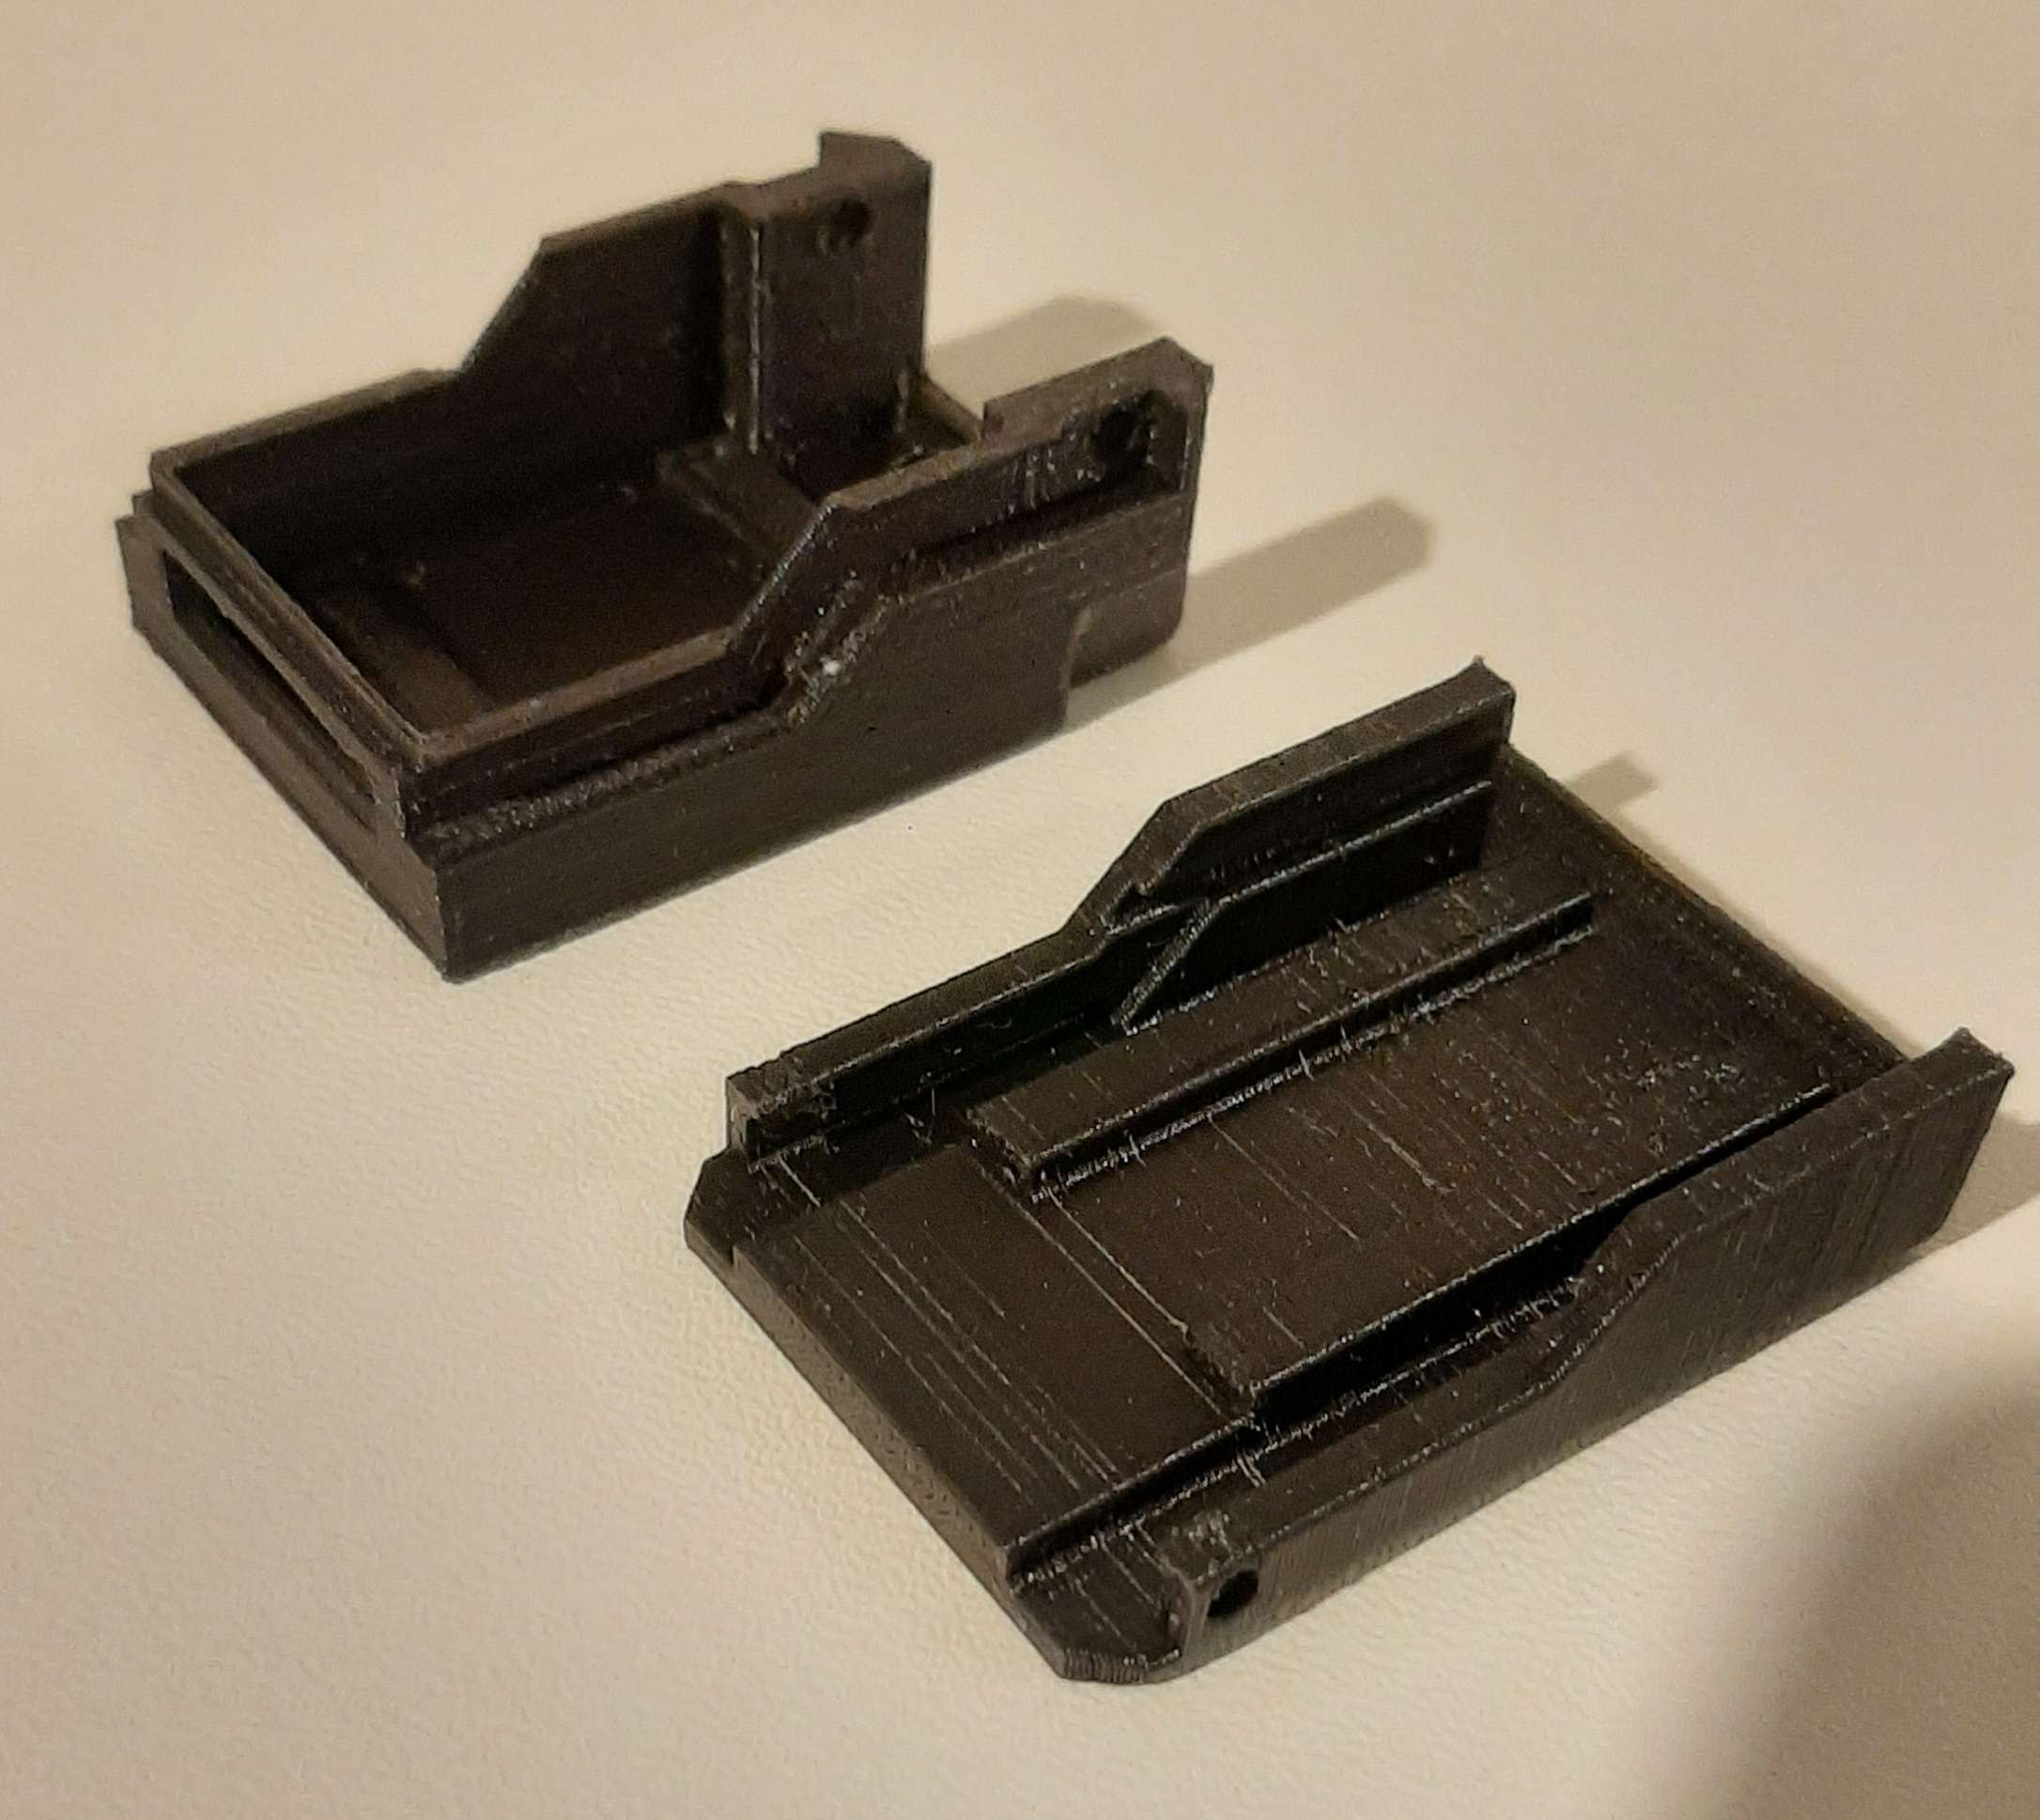
\includegraphics[scale=0.15]{obrazky/krabicka rozlozena.jpg}
    \end{center}
    \caption{Krabička čtečky čárového kódu - rozebrána}
    \label{Interakce mezi okny GUI}
\end{figure}

\begin{figure}[H]
    \begin{center}
        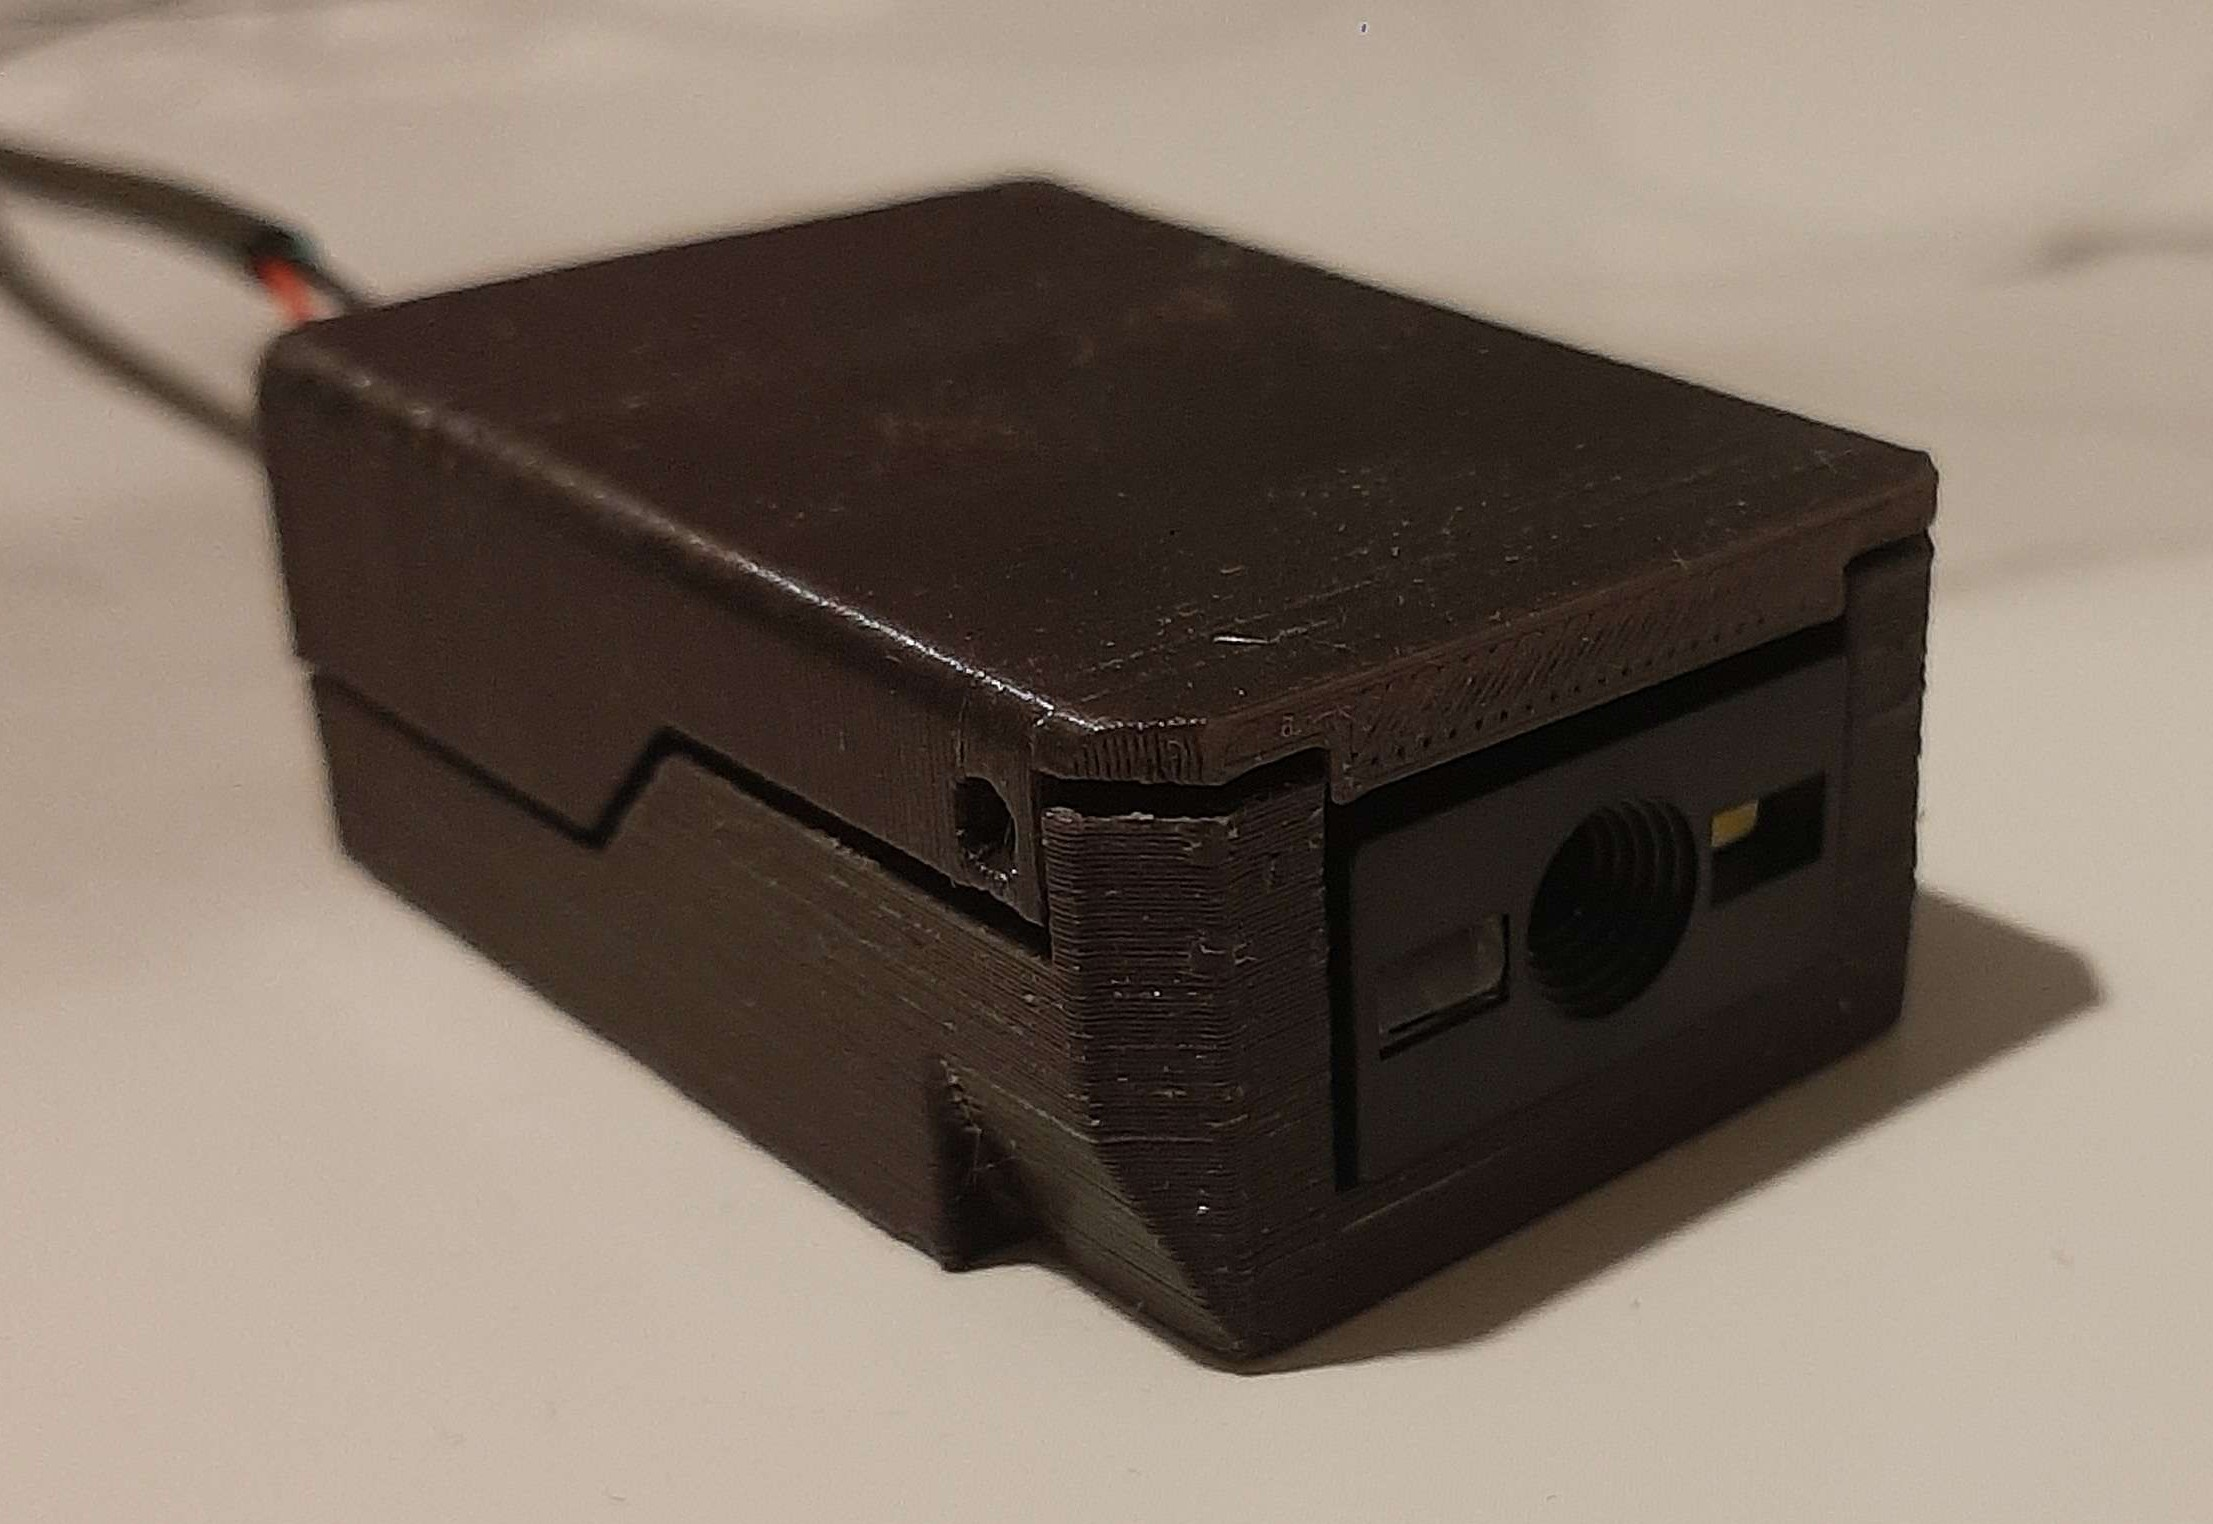
\includegraphics[scale=0.15]{obrazky/krabicka slozena.jpg}
    \end{center}
    \caption{Krabička čtečky čárového kódu - složena}
    \label{Interakce mezi okny GUI}
\end{figure}


//DODĚLAT DOKUMENTACI

\chapter{Naměřená data}

\section{Naměřené hmotnosti prázdných lahví}

\section{Tabulka naměřených objemů neotevřených lahví}

\begin{table}[h]
    \centering
    \begin{tabular}{|c|c|c|c|}
        \hline
         & \textbf{$m_{max}$ [g]} & \textbf{$m_{min}$ [g]} & \textbf{$m_{kap}$ [g]} \\ \hline \hline
        1 & 910.14 & 432.42 & 477.72 \\ \hline
        2 & 908.37 & 432.78 & 475.59 \\ \hline
        3 & 909.14 & 433.01 & 476.13 \\ \hline
        4 & 905.82 & 432.23 & 473.59 \\ \hline
        5 & 911.43 & 432.84 & 478.59 \\ \hline
        6 & 907.48 & 432.31 & 475.17 \\ \hline
        7 & 906.14 & 433.92 & 472.22 \\ \hline
        8 & 904.9 & 433.61 & 471.29 \\ \hline
        9 & 908.31 & 433.35 & 474.96 \\ \hline
        10 & 906.41 & 433.77 & 472.64 \\ \hline
        11 & 907.74 & 432.43 & 475.31 \\ \hline
        12 & 908.29 & 433.77 & 474.52 \\ \hline
        13 & 906.83 & 432.93 & 473.9 \\ \hline
        14 & 909.02 & 433.61 & 475.41 \\ \hline
        15 & 907.36 & 432.87 & 474.49 \\ \hline
    \end{tabular}
    \caption{Rozptyl hmotností plné ($m_{max}$), prázdné ($m_{min}$) láhve a jejich rozdíl ($m_{kap}$) - Amundsen vodka 0,5 l}
    \label{tab:chyba_lahve_a_plnění}
\end{table}


\section{Průběhy, výpočty a tabulky nárůstu hmotnosti z důvodu orosení}

\begin{equation}
T_{ds} = \frac{243,5 \cdot ln(\frac{V}{100} \cdot e^{\frac{17,67 \cdot T}{243,5 + T}})}{17,67 - ln(\frac{V}{100} \cdot e^{\frac{17,67 \cdot T}{243,5 + T}})}
\label{rosný bod obecne}
\end{equation}
%\caption{Rovnice rosného bodu}

\(T_{ds}\) ...Rosný bod \([\mathrm{^\circ C}]\)

\(V\) ...Relativní vlhkost vzduchu \([\mathrm{\%}]\)

\(T\) ...Teplota vzduchu \([\mathrm{^\circ C}]\)

\begin{equation}
T_{ds} = \frac{243,5 \cdot ln(\frac{50}{100} \cdot e^{\frac{17,67 \cdot 20}{243,5 + 20}})}{17,67 - ln(\frac{50}{100} \cdot e^{\frac{17,67 \cdot 20}{243,5 + 20}})} = 9,27 [^\circ C]
\label{rosný bod}
\end{equation}
%\caption{Požadavek na orosení T\_ds> 5 °C}

\bigskip

% Requires: \usepackage{graphicx}
\begin{table}[H]
    \centering
    \begin{tabular}{|c|c|c|c||c|c|c|}
    \hline
    \begin{tabular}[c]{@{}c@{}}čas \\ $[\text{min}]$\end{tabular} & 
    \begin{tabular}[c]{@{}c@{}}Božkov vaj. \\ lik. (0,5 l) [g]\end{tabular} & 
    \begin{tabular}[c]{@{}c@{}}Heffron \\ (0,7 l) [g]\end{tabular} & \begin{tabular}[c]{@{}c@{}}Nivnice \\ bor. (1 l) [g]\end{tabular} & 
    \begin{tabular}[c]{@{}c@{}}$\Delta$m \\ Božkov [g]\end{tabular} & \begin{tabular}[c]{@{}c@{}}$\Delta$m \\ Heffron [g]\end{tabular} & \begin{tabular}[c]{@{}c@{}}$\Delta$m \\ Nivnice [g]\end{tabular} \\ \hline \hline
    0  & 846.02 & 1190.02 & 1487.09 & 0.00 & 0.00 & 0.00 \\ \hline
    1  & 846.06 & 1190.03 & 1487.16 & 0.04 & 0.01 & 0.07 \\ \hline
    2  & 846.09 & 1190.05 & 1487.16 & 0.07 & 0.03 & 0.07 \\ \hline
    3  & 846.09 & 1190.09 & 1487.12 & 0.07 & 0.07 & 0.03 \\ \hline
    4  & 846.12 & 1190.09 & 1487.16 & 0.10 & 0.07 & 0.07 \\ \hline
    5  & 846.15 & 1190.12 & 1487.22 & 0.13 & 0.10 & 0.13 \\ \hline
    6  & 846.12 & 1190.22 & 1487.36 & 0.10 & 0.20 & 0.27 \\ \hline
    7  & 846.14 & 1190.21 & 1487.36 & 0.12 & 0.19 & 0.27 \\ \hline
    8  & 846.18 & 1190.22 & 1487.39 & 0.16 & 0.20 & 0.30 \\ \hline
    9  & 846.14 & 1190.25 & 1487.45 & 0.12 & 0.23 & 0.36 \\ \hline
    10 & 846.18 & 1190.31 & 1487.52 & 0.16 & 0.29 & 0.43 \\ \hline
    15 & 846.19 & 1190.32 & 1487.56 & 0.17 & 0.30 & 0.47 \\ \hline
    20 & 846.13 & 1190.35 & 1487.53 & 0.11 & 0.33 & 0.44 \\ \hline
    25 & 846.14 & 1190.31 & 1487.57 & 0.12 & 0.29 & 0.48 \\ \hline
    30 & 846.14 & 1190.37 & 1487.62 & 0.12 & 0.35 & 0.53 \\ \hline
    35 & 846.13 & 1190.38 & 1487.62 & 0.11 & 0.36 & 0.53 \\ \hline
    40 & 846.19 & 1190.47 & 1487.69 & 0.17 & 0.45 & 0.60 \\ \hline
    45 & 846.17 & 1190.41 & 1487.71 & 0.15 & 0.39 & 0.62 \\ \hline
    50 & 846.13 & 1190.46 & 1487.74 & 0.11 & 0.44 & 0.65 \\ \hline
    55 & 846.12 & 1190.39 & 1487.68 & 0.10 & 0.37 & 0.59 \\ \hline
    60 & 846.12 & 1190.30 & 1487.67 & 0.10 & 0.28 & 0.58 \\ \hline
    \end{tabular}
    %\caption{Vliv orosení na hmotnost láhve}
    \caption{Změna hmotnosti lahve vlivem orosení}
    \label{tab:measurement_data}
\end{table}

\begin{figure}[H]
    \begin{center}
        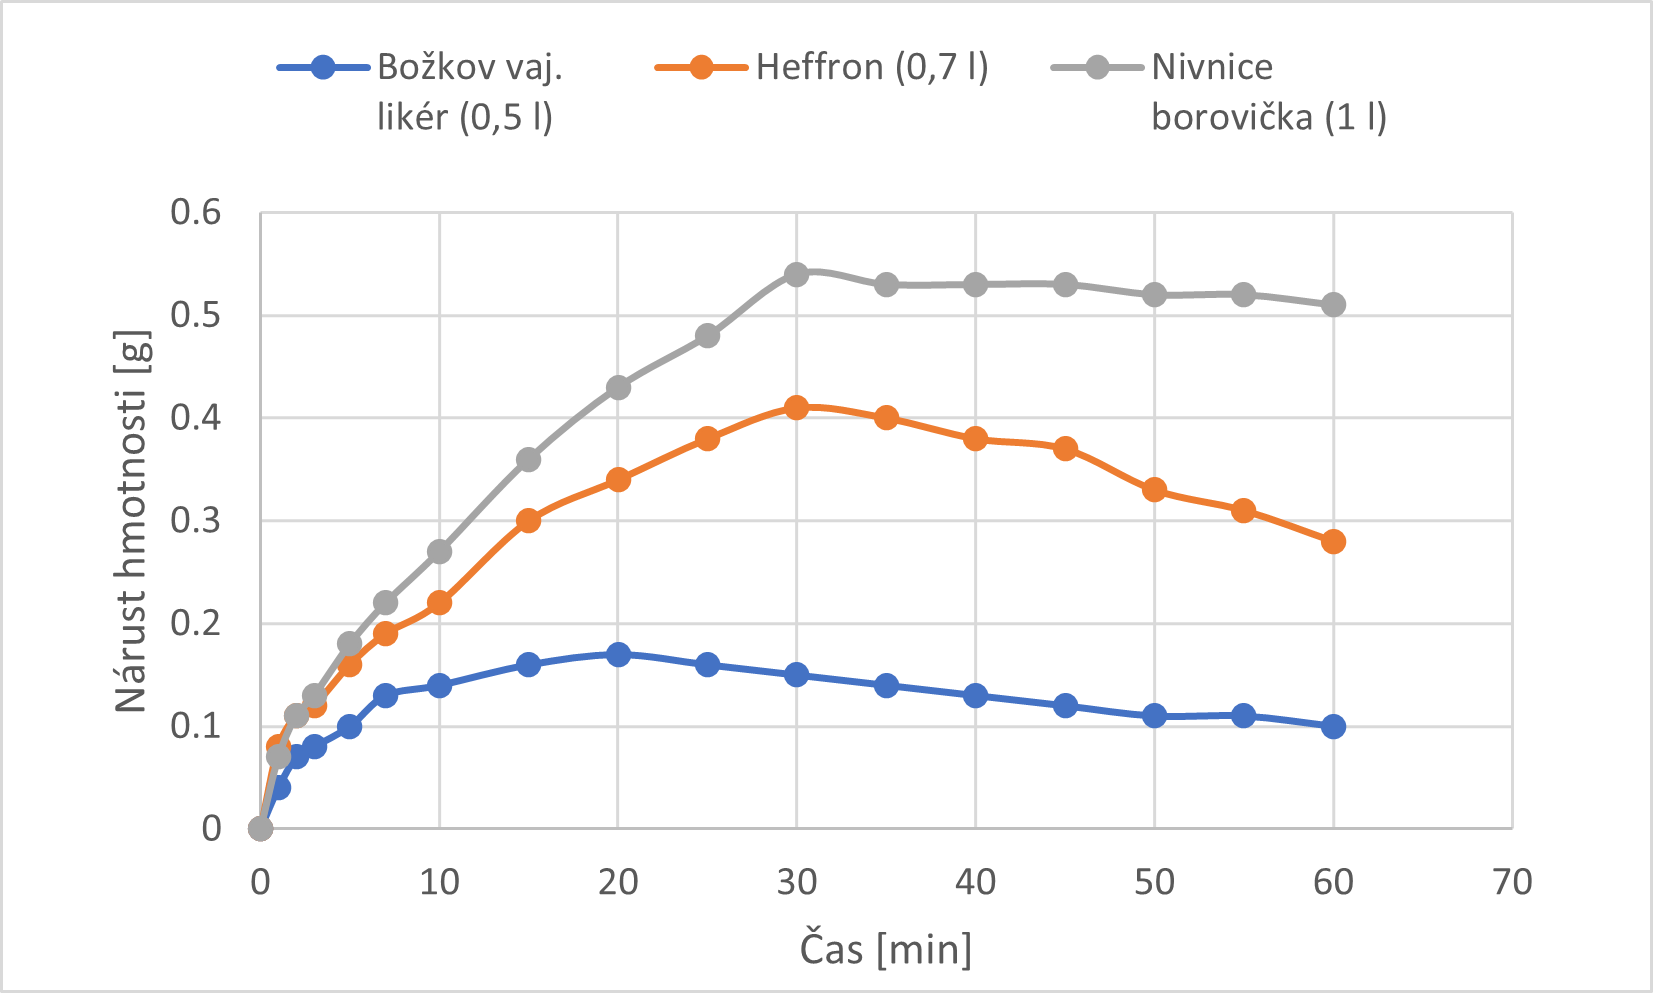
\includegraphics[scale=1.2]{obrazky/orosení.png}
    \end{center}
    \caption{Nárůst hmotnosti při orosení láhve}
\end{figure}

\chapter{Ostatní okna grafického prostředí firemwaru}

\begin{figure}[!h]
    \begin{center}
        
\includegraphics[scale=0.22]{obrazky/GUI Spuštění inventury.png}
        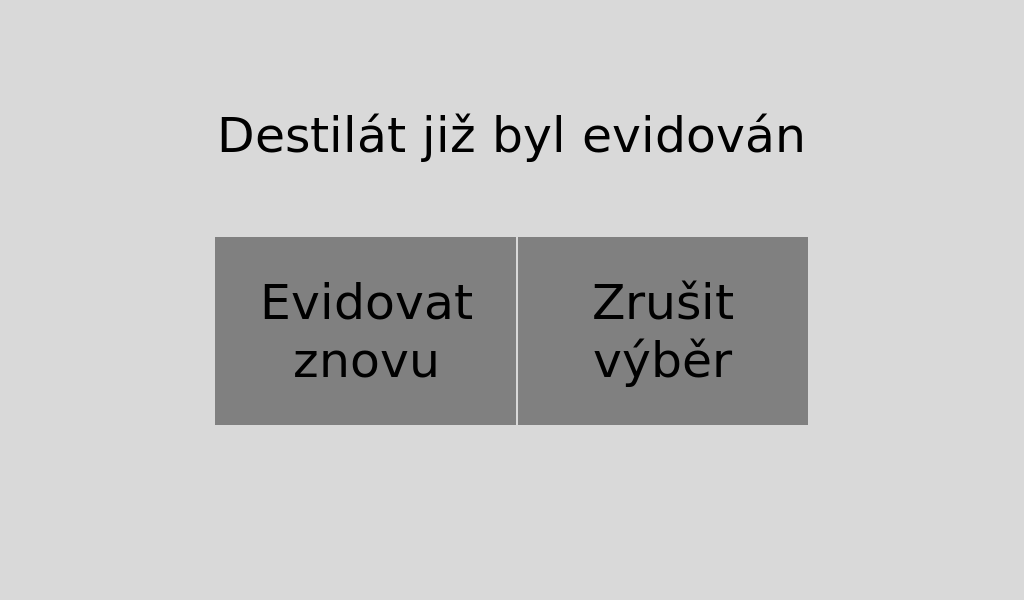
\includegraphics[scale=0.22]{obrazky/GUI Duplicidita.png}  
    \end{center}
    \caption{Úvodní okno firemwaru}
    \label{Úvodní okno aplikace}
\end{figure}

%\begin{figure}[H]
%    \begin{center}
%        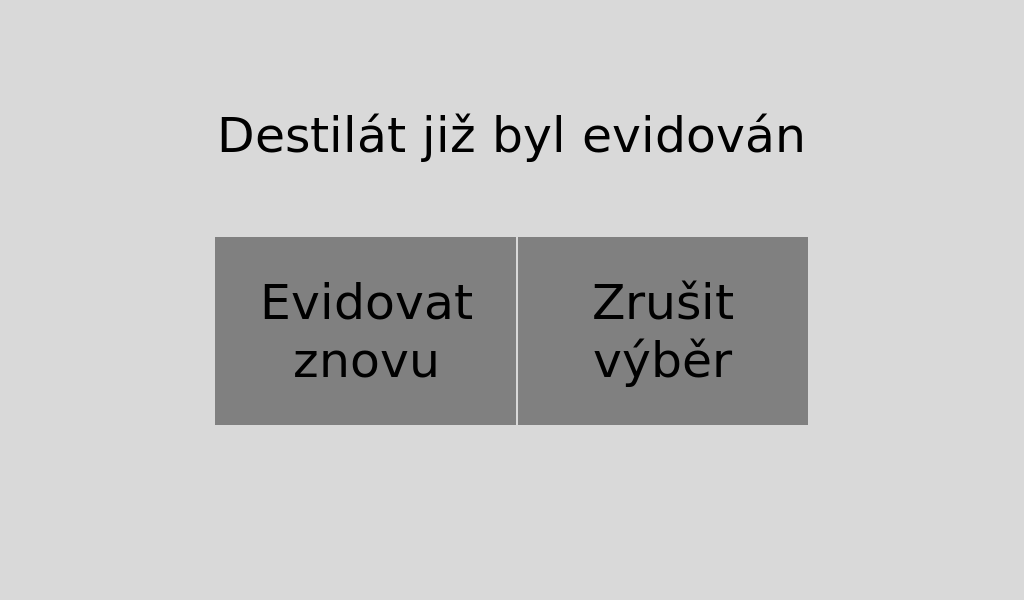
\includegraphics[scale=0.4]{obrazky/GUI Duplicidita.png}
%    \end{center}
%    \caption{Okno informující o duplicitní evidenci produktu}
%    \label{Okno informující o duplicitní evidenci produktu}
%\end{figure}

\begin{figure}[H]
    \begin{center}
        \includegraphics[scale=0.2]{obrazky/GUI Nastavení.png}
        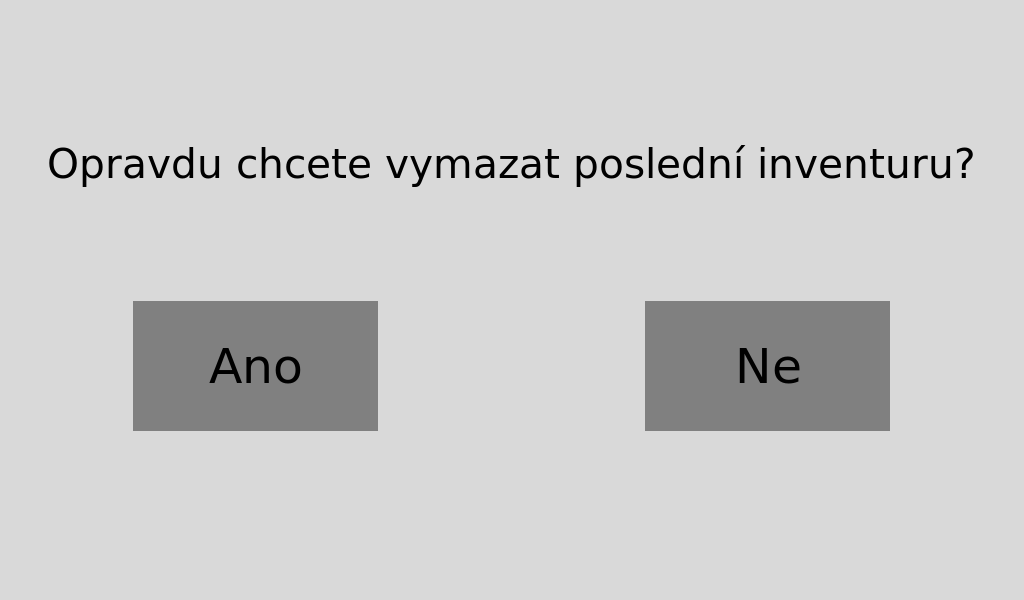
\includegraphics[scale=0.2]{obrazky/GUI Vymazání inventury.png}
    \end{center}
    \caption{Okno s nastavením firemwaru}
    \label{Okno s nastavením aplikace}
\end{figure}

\begin{figure}[H]
    \begin{center}
        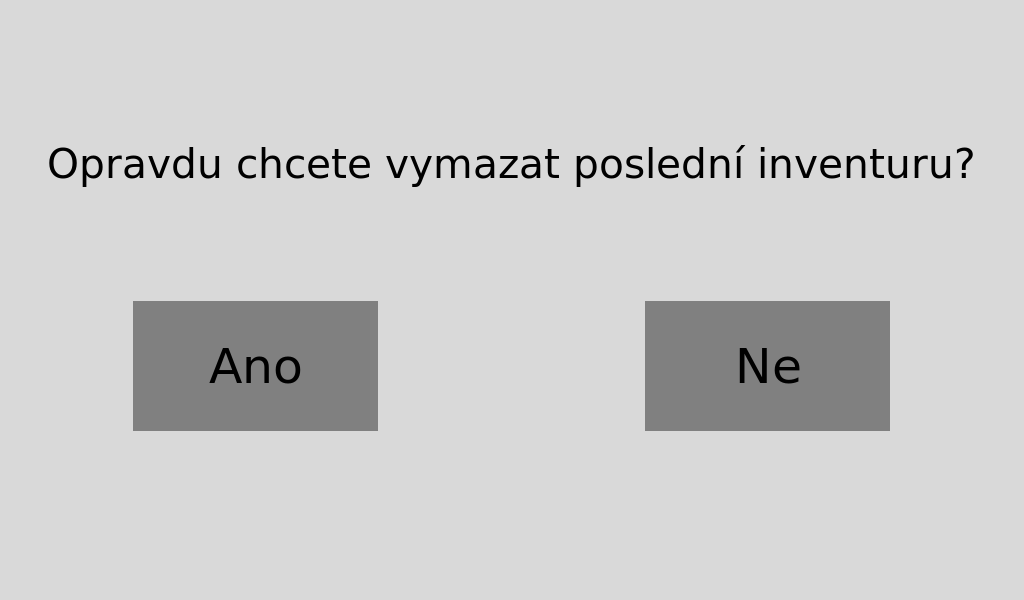
\includegraphics[scale=0.4]{obrazky/GUI Vymazání inventury.png}
    \end{center}
    \caption{Potvrzovací okno pro vymazání aktuálně spuštěné inventury}
    \label{Potvrzovací okno pro vymazání aktuálně spuštěné inventury}
\end{figure}



\chapter{Příručka GUI}


\end{document}